\providecommand{\main}{..}
\documentclass[\main/thesis.tex]{subfiles}

\begin{document}

\chapter{Microworld Experiments}

The goal in this section is to understand differences between FKL and RKL in terms of (1) the loss surface and (2) the behaviour of iterates optimized under the losses. By behaviour, we mean whether the iterates reach multiple local optima, how stable iterates under that loss are, and how often iterates reach the global optimum (or optima). Given the fine-grained nature of our questions, we focus upon small-scale environments, which we call \textit{microworlds}. Doing so allows us to avoid any possible confounding factors associated with larger, more complicated environments, and furthermore allows us more fully to separate any issues to do with stochasticity. 

We begin with continuous actions, and note results for discrete actions in \Cref{sec:microworld-discrete-actions}. We use two types of low-dimensional microworlds to allow us to visualize and thoroughly investigate behavior.

Our first microworld is a \textbf{Bimodal Bandit} in \Cref{fig:bimodal-bandit}. For continuous actions, we designed a continuous bandit with action space $[-1, 1]$ and reward function $Q(a) := \exp( -\tfrac{1}{2} (\tfrac{2 a + 1}{0.2})^2 ) + \tfrac{3}{2} \exp(-\tfrac{1}{2} (\tfrac{2 a - 1}{0.2})^2)$. The two unequal modes at -0.5 and 0.5 enable us to test the mean-seeking and mode-seeking behavior as well as simulate a realistic scenario where the agent's policy parameterization (here, unimodal) cannot represent the true distribution (bimodal). For discrete actions, we designed a discrete bandit with rewards $(1, 1.5)$. 

Our second microworld is the \textbf{Switch-Stay} domain in \Cref{fig:switch-stay}. From $s_0$, action $0$ (stay) gives a reward of 1 and transitions to state $0$. From $s_1$, action 0 gives a reward of 2 and transitions to $s_1$. From $s_0$, action 1 (switch) gives a reward of -1 and transitions to $s_1$, while action 1 from $s_1$ gives a reward of 0 and transitions to $s_0$. 

To adapt this environment to the continuous action setting, we treat actions $> 0$ as switch and actions $\leq 0$ as stay.  We set $\gamma = 0.9$ to ensure that the optimal action from $s_0$ is to switch, which ensures the existence of a short-term/long-term trade-off inherent to realistic RL environments. 

\begin{figure}[!htb]
  \hspace*{10em}\resizebox{0.4\columnwidth}{!}{%
\begin{tikzpicture}[auto,node distance=10mm,>=latex,font=\small]
    \tikzstyle{round}=[thick,draw=black,circle]

    \node[round] (s0) {$s_0$};
    \node[round,right=20mm of s0] (s1) {$s_1$};

    \draw[->] (s0) to [out=45, in=135] node {-1} (s1);
    \draw [->] (s0) to [out=135,in=225, loop] node {1} (s0);
    \draw [->] (s1) to [out=210,in=330] node{0} (s0);
    \draw [->] (s1) to [out=45,in=-45, loop] node {2} (s1);
\end{tikzpicture}}
    \caption{Switch-Stay.}
    \label{fig:switch-stay}
\end{figure}%

\begin{figure}[!htb]
    \centering
    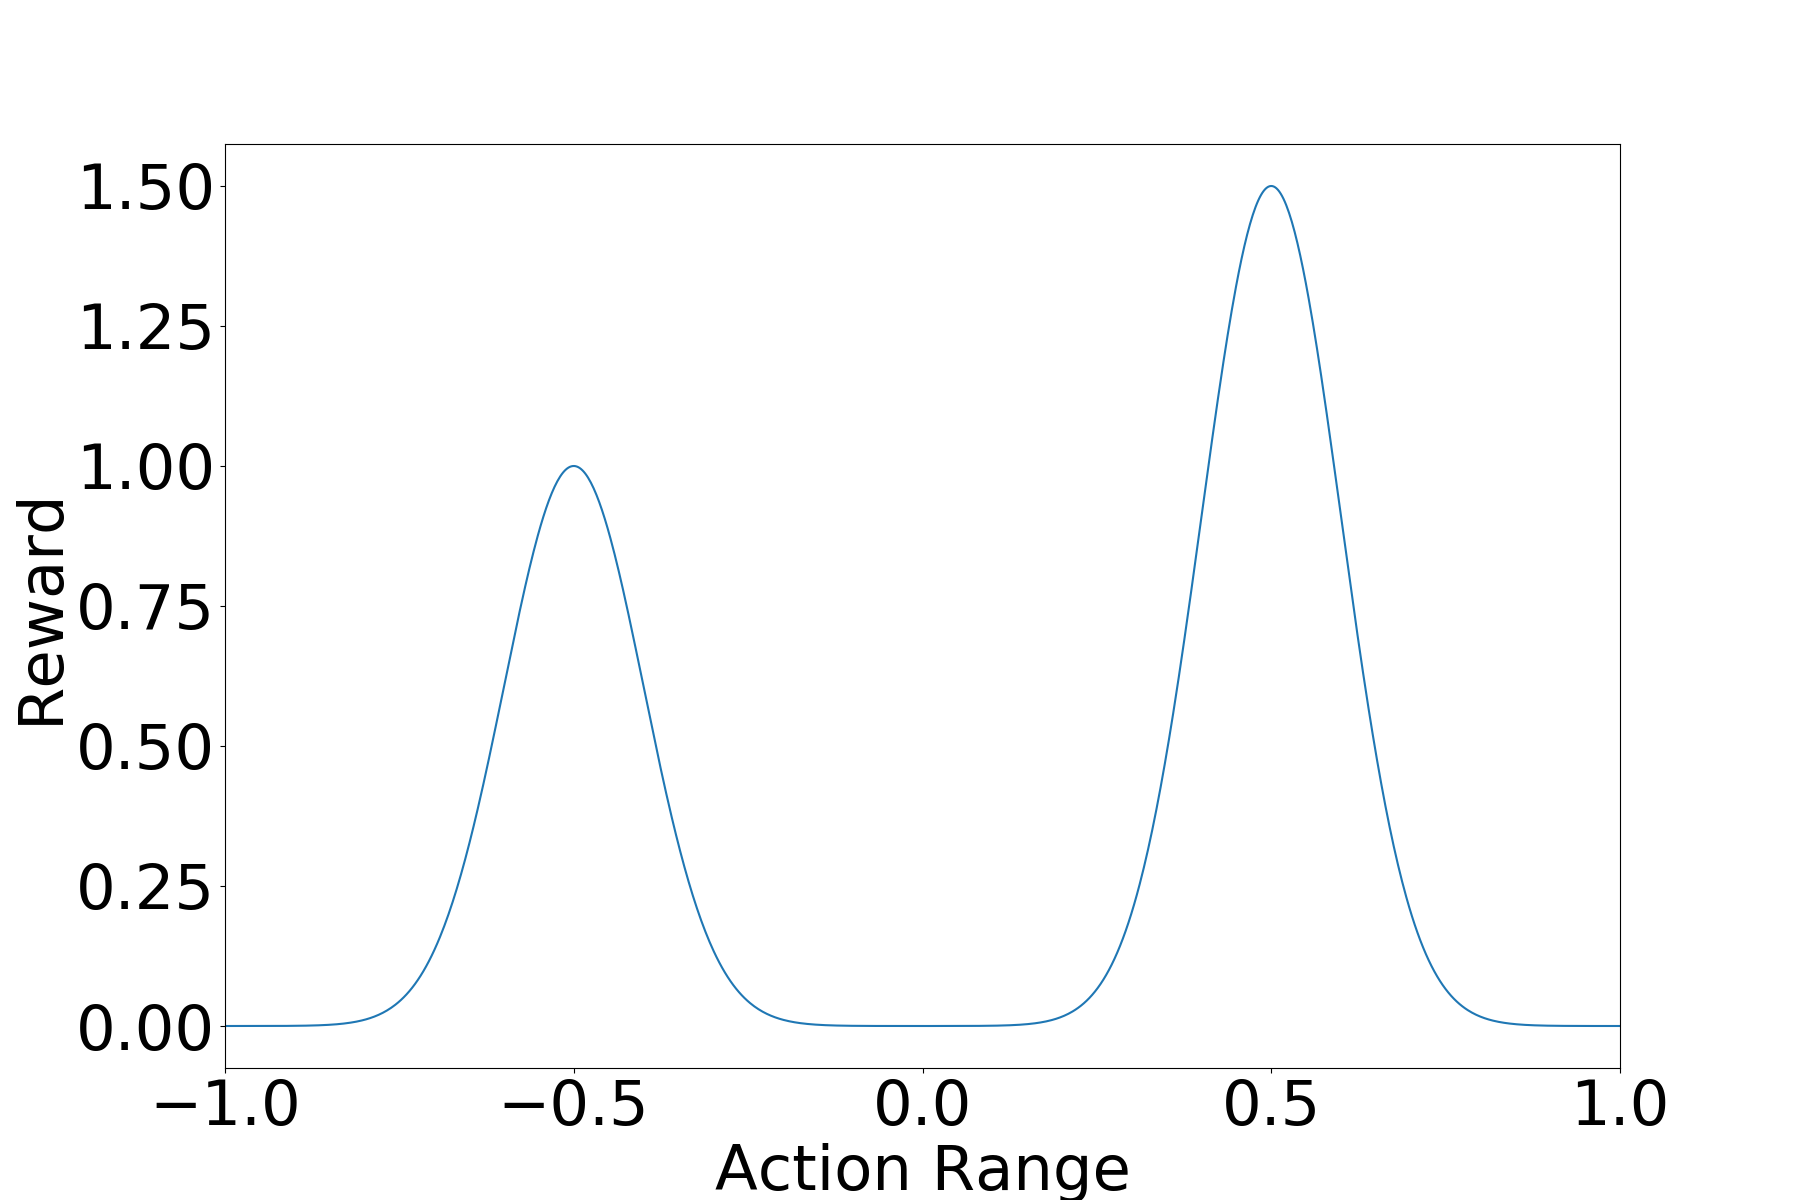
\includegraphics[width=0.7\linewidth]{figs/bandit/bimodal-bandit.png}
    \caption{Continuous-action Bimodal Bandit.}
    \label{fig:bimodal-bandit}
\end{figure}


% \textbf{Common Implementation Details}
\section{Common Implementation Details}
\noindent All policies are tabular in the state. To calculate the FKL and RKL for the continuous action setting, we use the Clenshaw-Curtis \citep{clenshaw1960method} numerical integration scheme with 1024 points from the package quadpy \citep{schlomerquadpy}, excluding the first and the last points at -1 and 1 because of numerical stability. Numerical integration is used to minimize any confounding influence of stochasticity on the behaviour, but we also note additional results for Monte Carlo integration in \Cref{sec:stochastic-microworld}.

To calculate the Hard FKL, we use the true maximum action as determined by the environment. In the discrete action setting, we may calculate the non-hard FKL losses in closed form by summing across all actions. For Switch-Stay, we calculate and optimize the mean KL across the two states.

We use the true action-values when calculating the KL losses; in the bimodal bandit, the action-value is given by the reward function, while in Switch-Stay it is calculated (i.e., not learned). For policy parameterizations, in continuous action settings we use a Gaussian policy with mean and variance learned as $(\hat{\mu}, \log(1+\exp(\hat{\sigma}))$ and in discrete action settings we use a softmax policy. The action sampled from the learned Gaussian is passed through $\tanh$ to ensure that the action is in the feasible range $[-1, 1]$ and to avoid the bias induced in the policy gradient when action ranges are not enforced \citep{chou2017improving}. 

Finally, we use the RMSprop optimizer \citep{tieleman2012lecture}. Overall trends for Adam \citep{kingma2014adam} were similar to those for RMSprop, while results for SGD resulted in slower learning for both FKL and RKL and a wider range of limit points, most likely due to oscillation from the constant step-size. We focus on RMSprop here to avoid any confounding factors associated with momentum. 


\section{Continuous Action Results in the Bimodal Bandit}
Firstly, we might expect the FKL to have a smoother loss surface. Given that policies often are part of an exponential class (e.g., softmax policy), having the policy $\pi$ be the second argument of $\KL(p \parallel q)$ might be advantageous as $\KL(p \mid \pi)$ removes the exponential in $\pi$. 

\subsection{Loss Surface}
% \myparagraph{Optimization Surface for the Bimodal Bandit}
We visualize the KL loss surfaces in \Cref{fig:bandit-heatmap} with five different temperatures. The heatmaps depict the loss for each mean and standard deviation pair. The last row depicts the target distribution over which the KL loss is optimized. The surfaces suggest the following. 

\textbf{1)} The FKL surface has a single valley, while the RKL surface has two valleys that are separated from one another. In this sense, the FKL surface seems much smoother than the RKL surface, suggesting that iterates under the FKL will more likely reach the global optimum than iterates under the RKL, which seem likely to fall into either of the valleys. 

\textbf{2)} The smoothness of the RKL landscape increases with temperature as the gap between the peaks becomes less steep. A higher temperature also causes the valley in the FKL map to become less sharply peaked, and for the optimal $\mu$ to move closer to 0. The optimal $\mu$ for the FKL seems to move more quickly to zero, as $\tau$ increases, than the optimal $\mu$ for the RKL, although both eventually reach 0. It is possible that the FKL may become suboptimal sooner than the RKL as $\tau$ increases. 

\textbf{3)} It may seem strange that two valleys exist for the RKL at $\tau = 0$ given that the target distribution is unimodal. Note, however, that when $\tau = 0$, the loss function is no longer a distributional loss; that is, we are no longer minimizing any pseudo-distance between the policy and a distribution. 


% \textbf{3)} As the temperature decreases, the target distribution becomes unimodal; making the mean and the mode become identical; the global optimum for both the FKL and RKL is at the optimal peak.

% We also considered the effects of numerical integration and the $\tanh$ transformation.
% \textbf{6)} FKL seems to be more robust to numerical integration error. When reducing the number of integration points, there was no visible difference in the FKL loss surface but wavelet patterns are observed in the RKL loss surface (Appendix H).
% \textbf{7)} The optimization surface for a Gaussian policy without the $\tanh$ transformation is shown in Appendix H. In this setting, suboptima appear along the edges in all soft RKL surfaces, while FKL loss surface seems unaffected.

\begin{figure}[!htb]
    \centering
    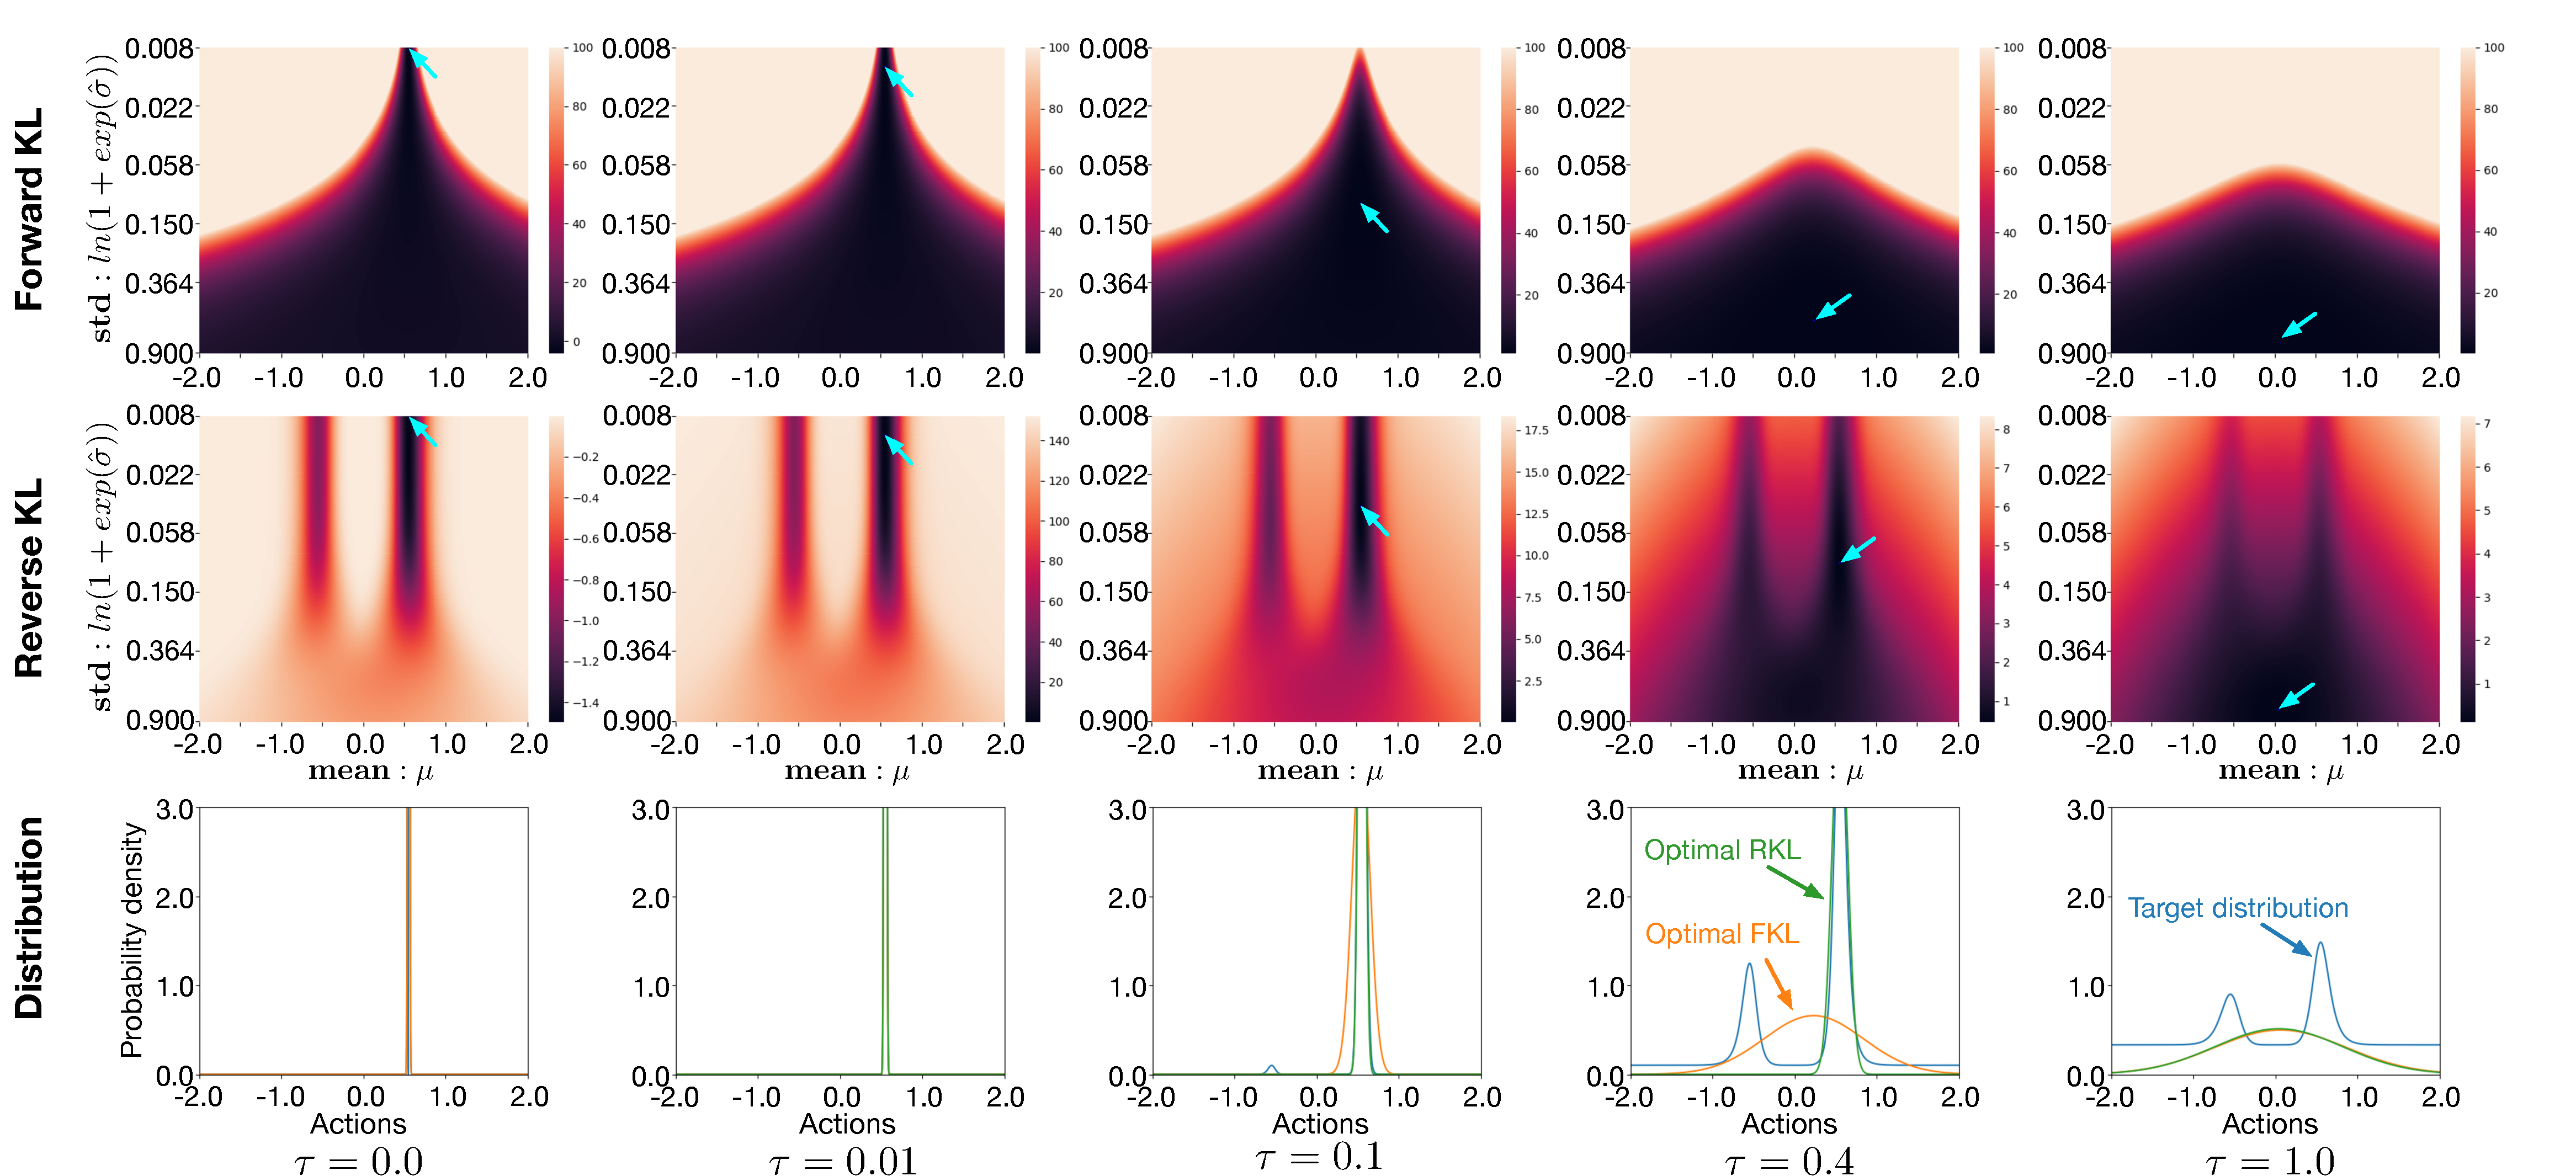
\includegraphics[width=0.99\columnwidth]{figs/bandit/trueQ/heatmaps/heatmap_combined.pdf}
    \caption{KL loss over mean and standard deviation across temperature. Note that the actual action taken applies $\tanh$ to the samples of the resulting distribution (i.e., the optimal mean is at $\tanh^{-1}(0.5) \approx 0.55$). FKL loss has been upper-bounded for better visualization of minima. Arrows indicate the global minimum.}
    \label{fig:bandit-heatmap}
\end{figure}

% \begin{figure}[!htb]
%   \centering
%   \begin{subfigure}[b]{1\linewidth}
%     \centering
%     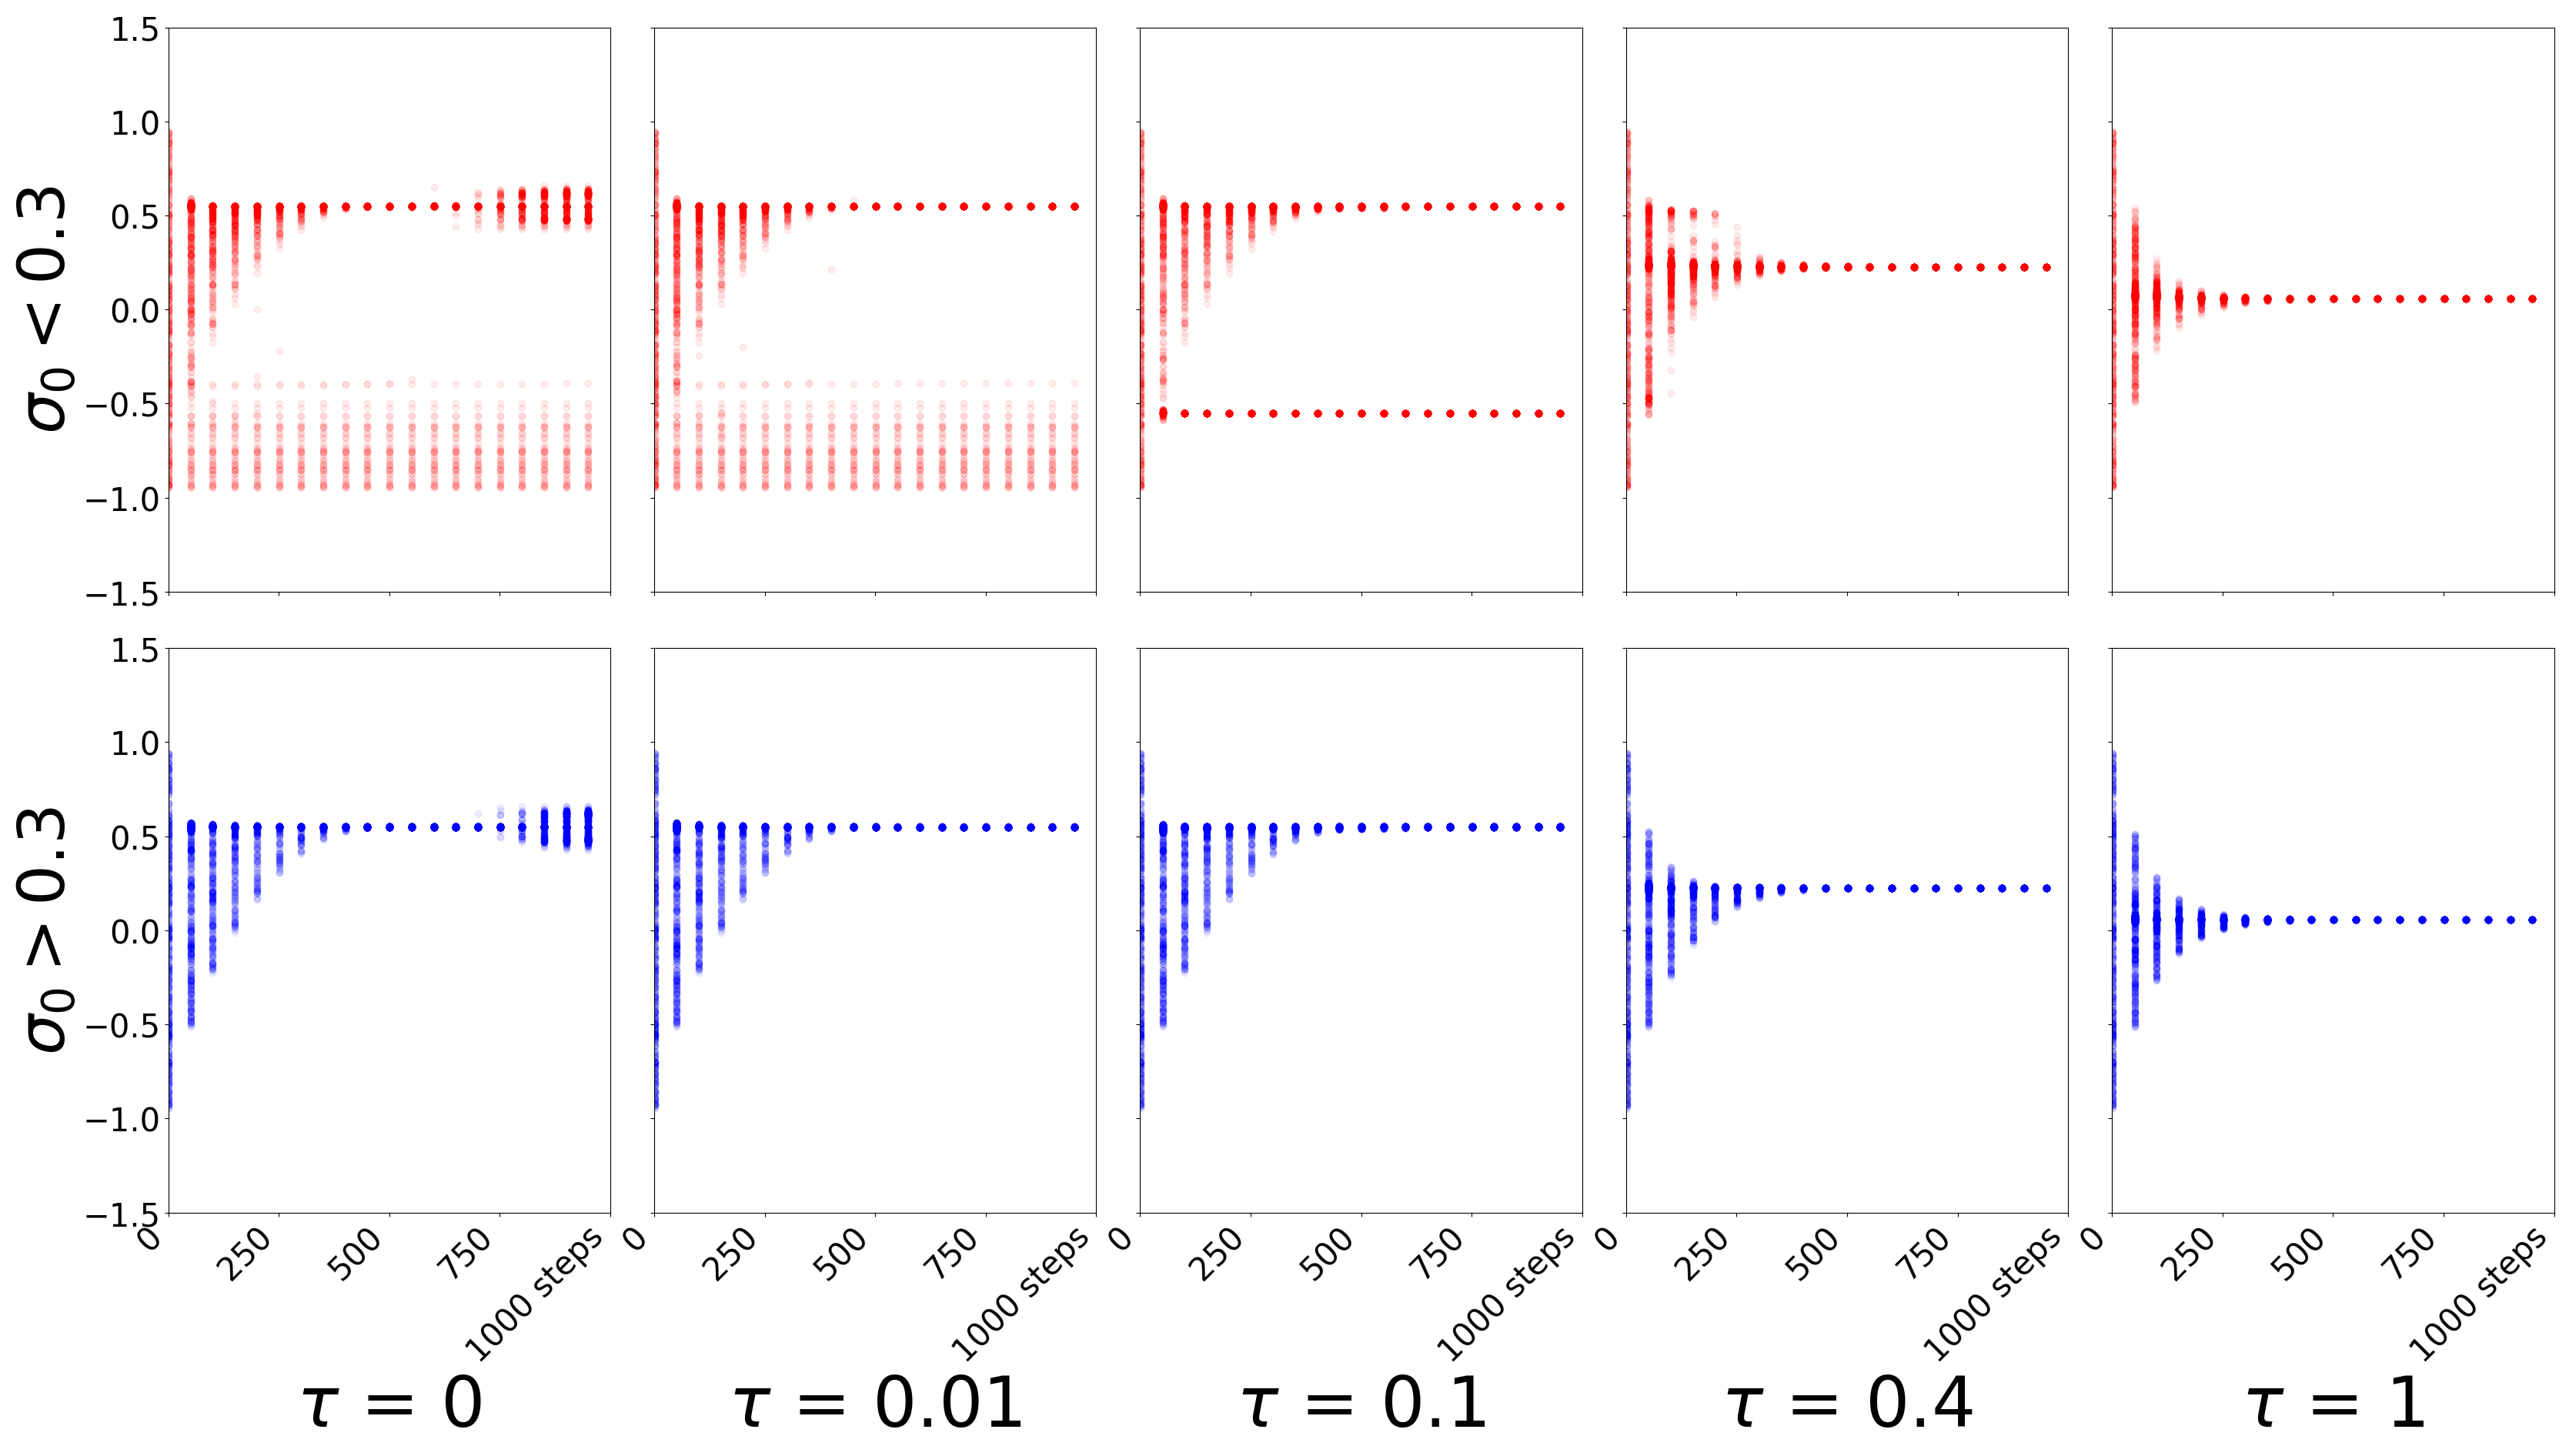
\includegraphics[width=\columnwidth]{figs/bandit/notlearnQ/modes=1/adam/mean_forward_optim=adam_modes=1_lr=0.01.png}
%     \caption{Forward KL.}
%     \label{fig:bandit-mean-forward-adam}
%   \end{subfigure}
  
%   \begin{subfigure}[b]{1\linewidth}
%     \centering
%     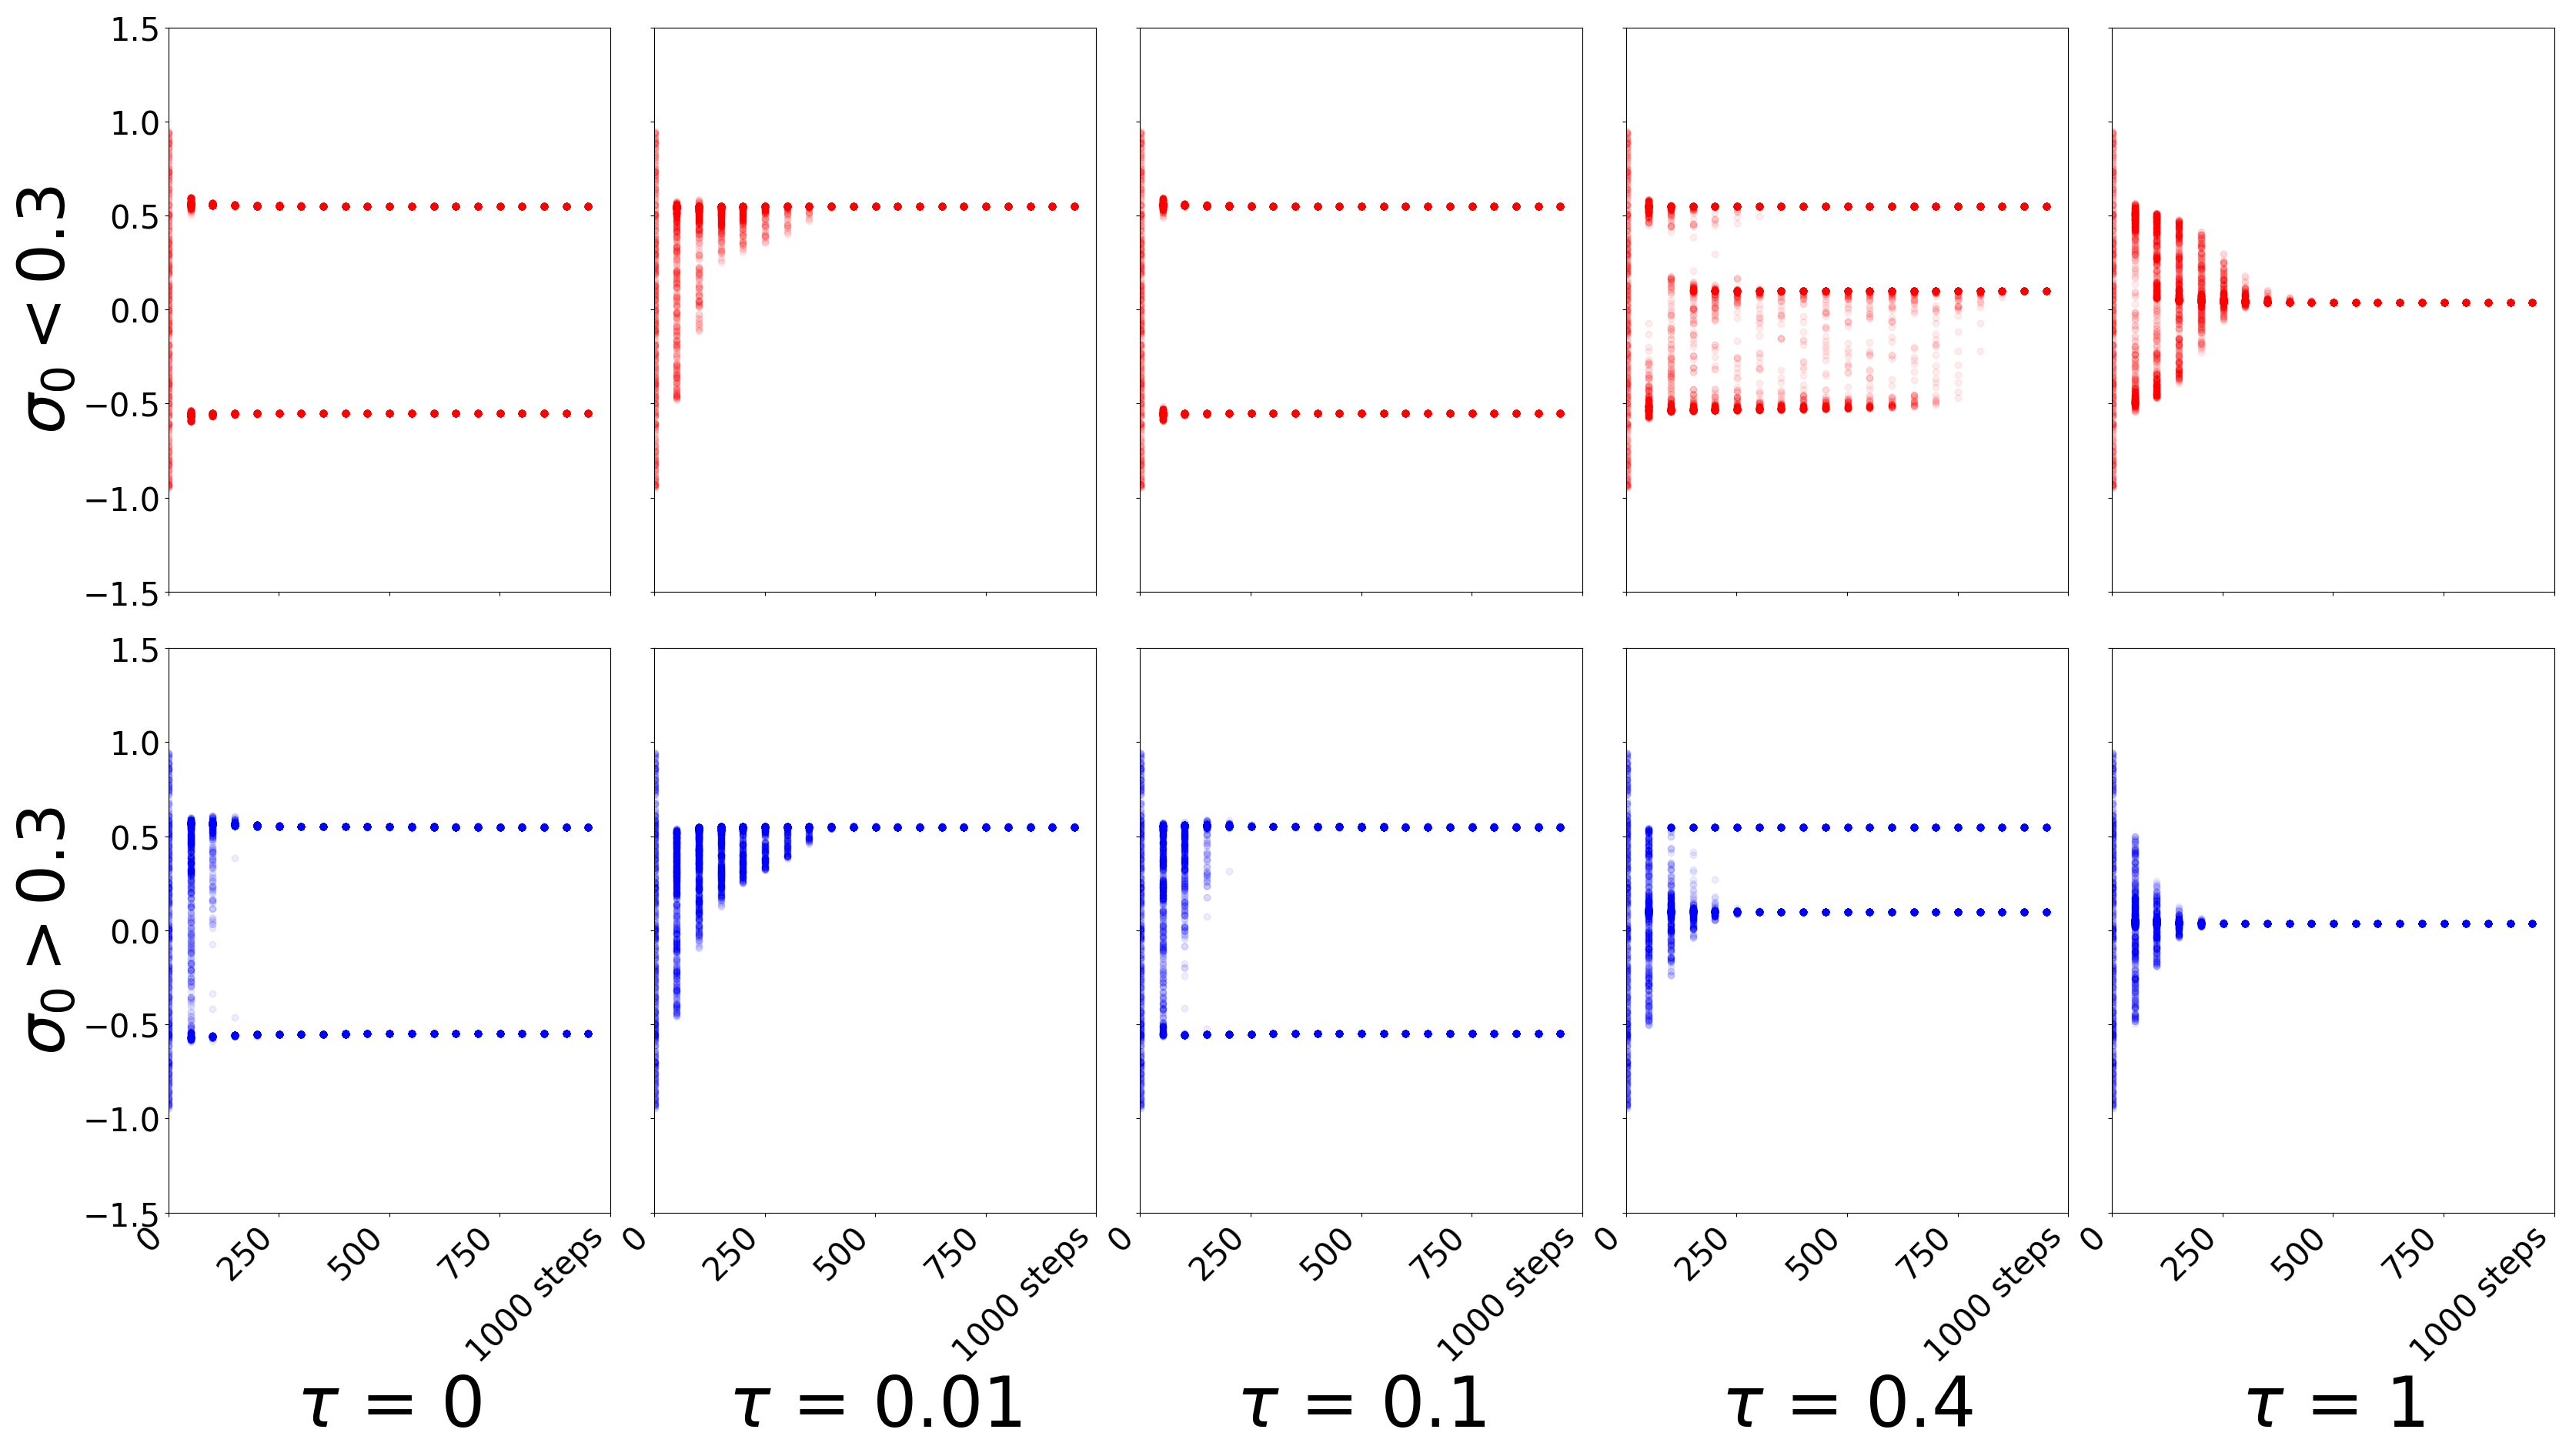
\includegraphics[width=\columnwidth]{figs/bandit/notlearnQ/modes=1/adam/mean_reverse_optim=adam_modes=1_lr=0.01.png}
%     \caption{Reverse KL.}
%     \label{fig:bandit-mean-reverse-adam}
%   \end{subfigure}
%   \caption{Each plot tracks the mean over 1000 gradient steps of each of 1000 iterates. Each iterate is represented as a translucent, coloured dot with alpha value $0.01$. Temperature is varied on the $x$-major-axis and initial standard deviation $\sigma_0$ is varied on the $y$-major axis. Colour-coded by $\sigma_0$.}
% \end{figure}

\subsection{Behaviour}
To confirm whether our intuitions about the smooth loss surface result in iterates that reach the global optimum, we visualize 1000 random (mean, standard deviation) iterates over 1000 gradient steps to minimize either the FKL or RKL. The mean is initialized uniformly in $(-0.95, 0.95)$ and $\hat{\sigma}$ is initialized uniformly in $(\log(\exp(0.1) - 1), \log(\exp(1) - 1))$, so that the initial standard deviation $\sigma_0$ is in $(0.1, 1)$. We only show one learning rate, but results are similar for different learning rates. From looking at \Cref{fig:bandit-mean-forward-rmsprop,fig:bandit-mean-reverse-rmsprop}, we observe the following.

\begin{figure}[!htb]
  \centering
  \begin{subfigure}[b]{1\linewidth}
    \centering
    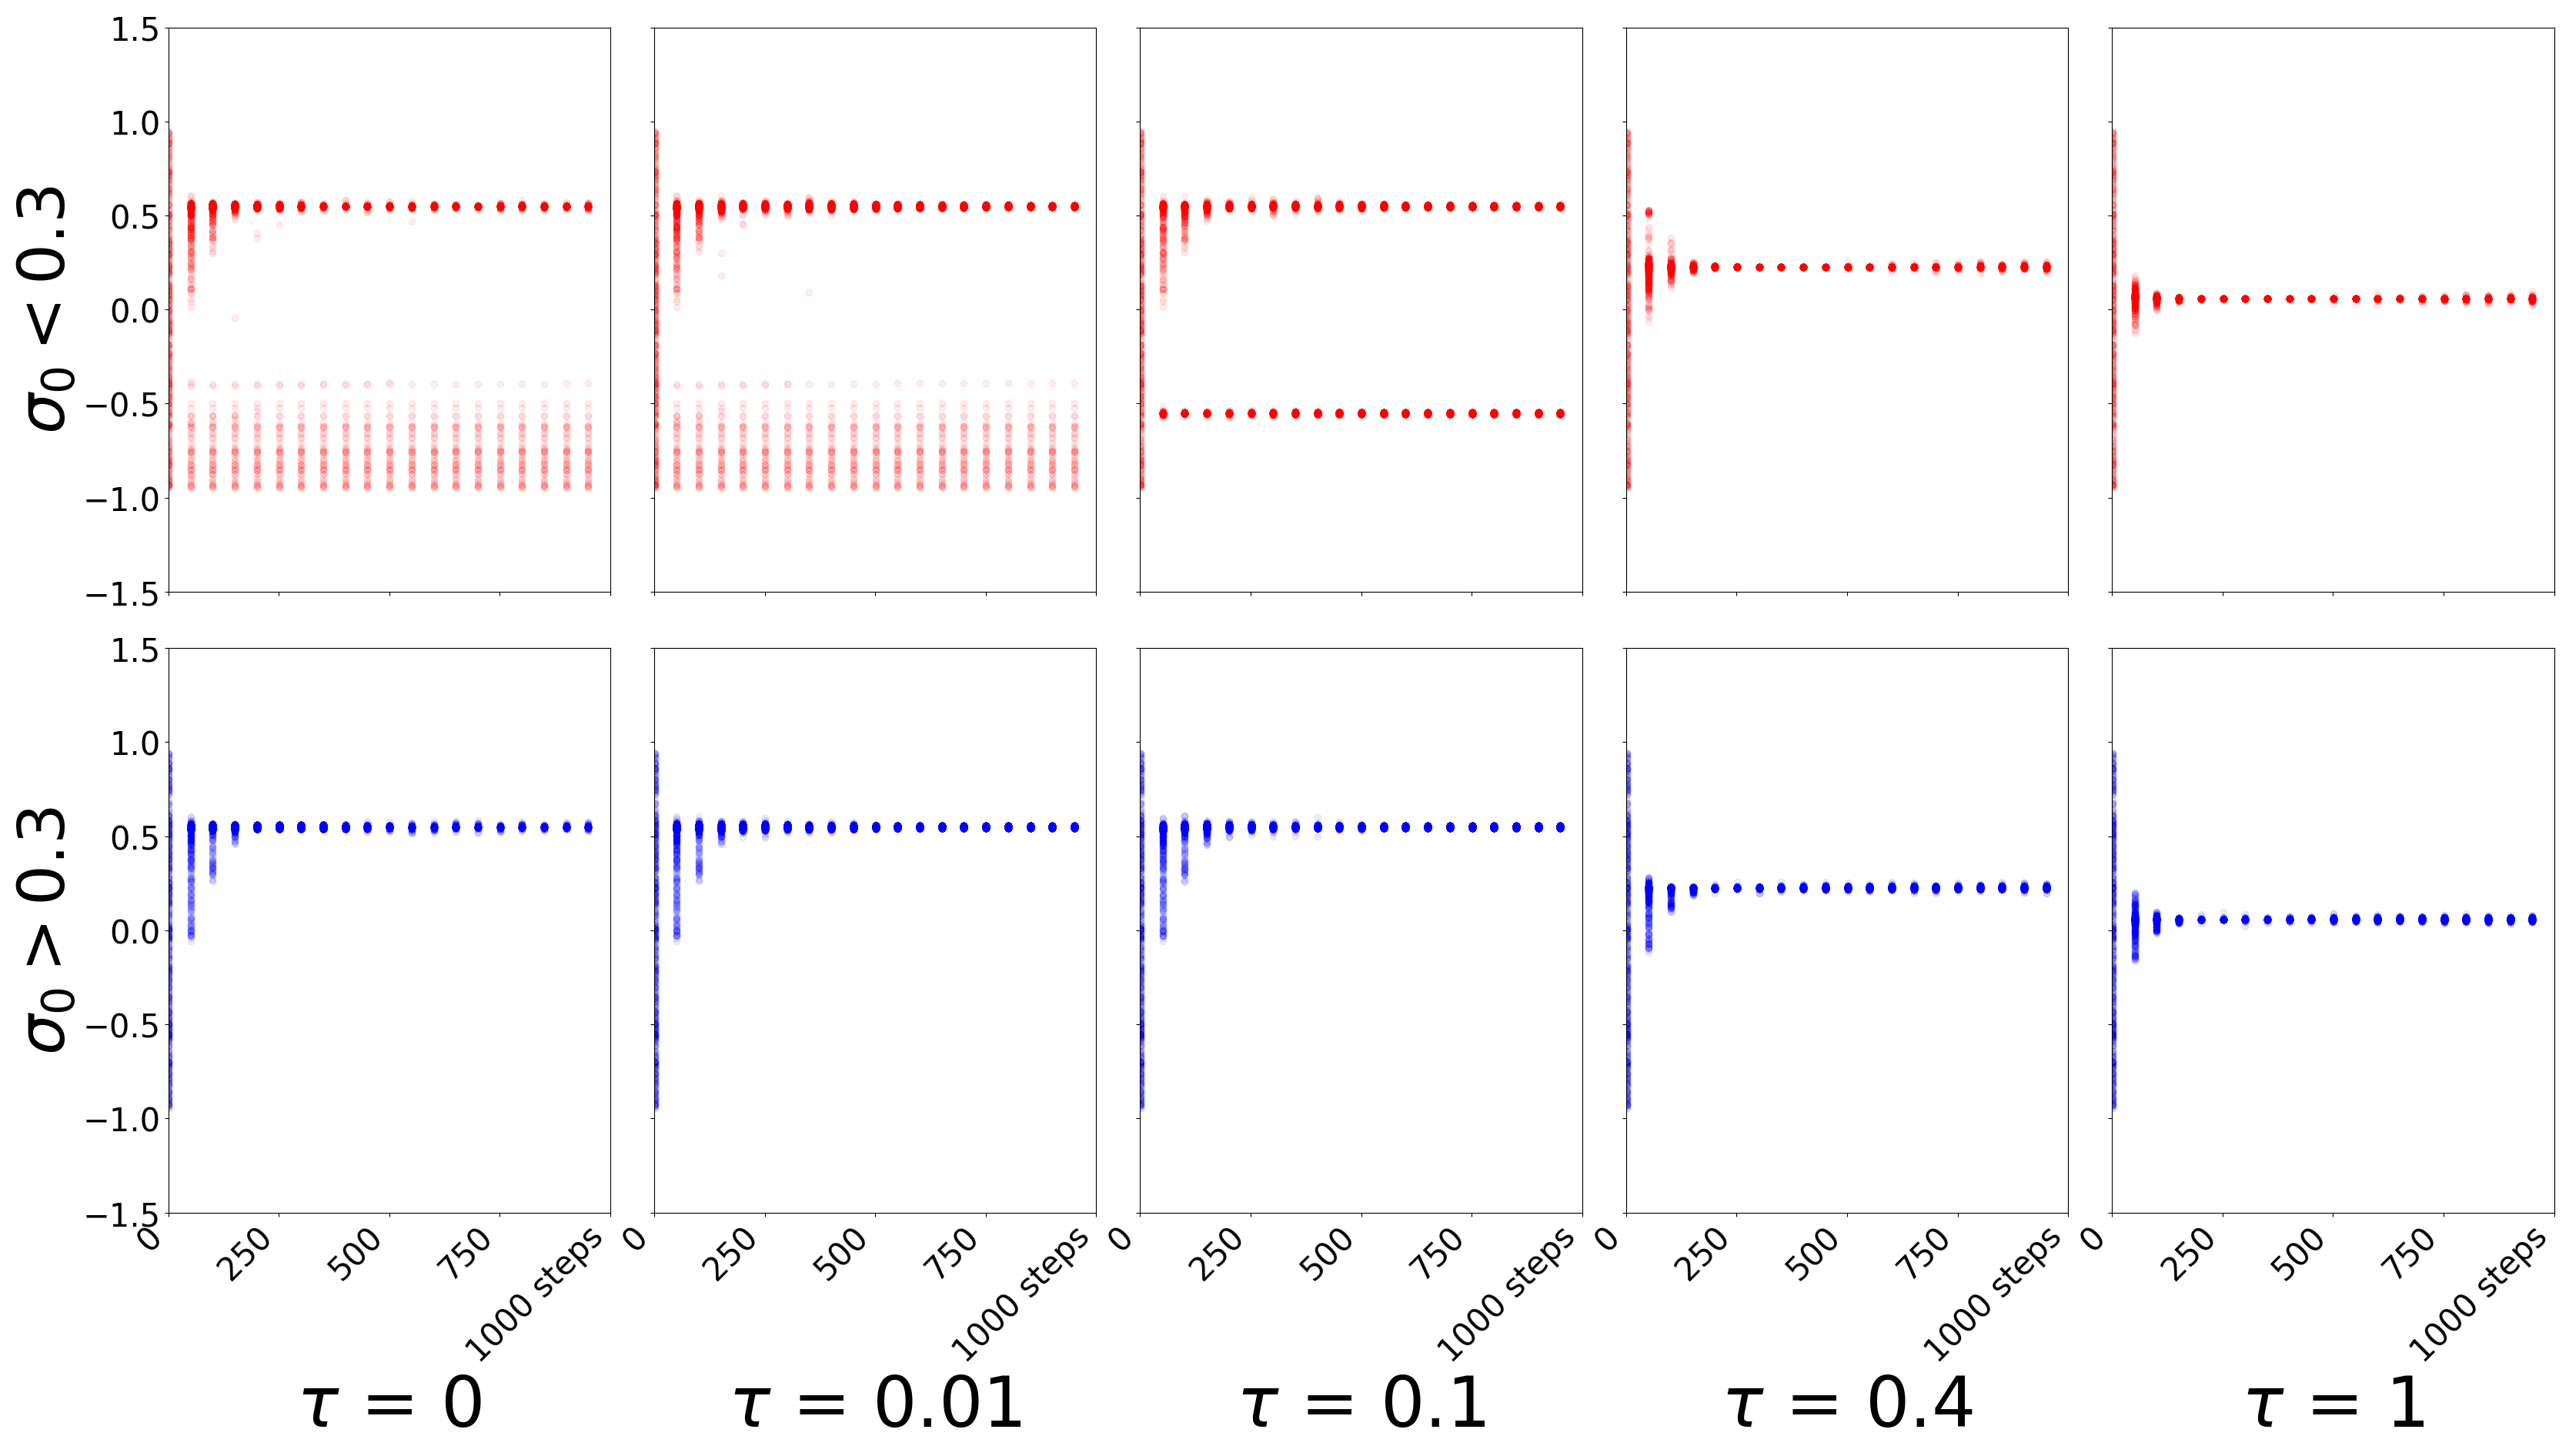
\includegraphics[width=\columnwidth]{figs/bandit/notlearnQ/modes=1/rmsprop/mean_forward_optim=rmsprop_modes=1_lr=0.01.png}
    \caption{Forward KL.}
    \label{fig:bandit-mean-forward-rmsprop}
  \end{subfigure}
  
  \begin{subfigure}[b]{1\linewidth}
    \centering
    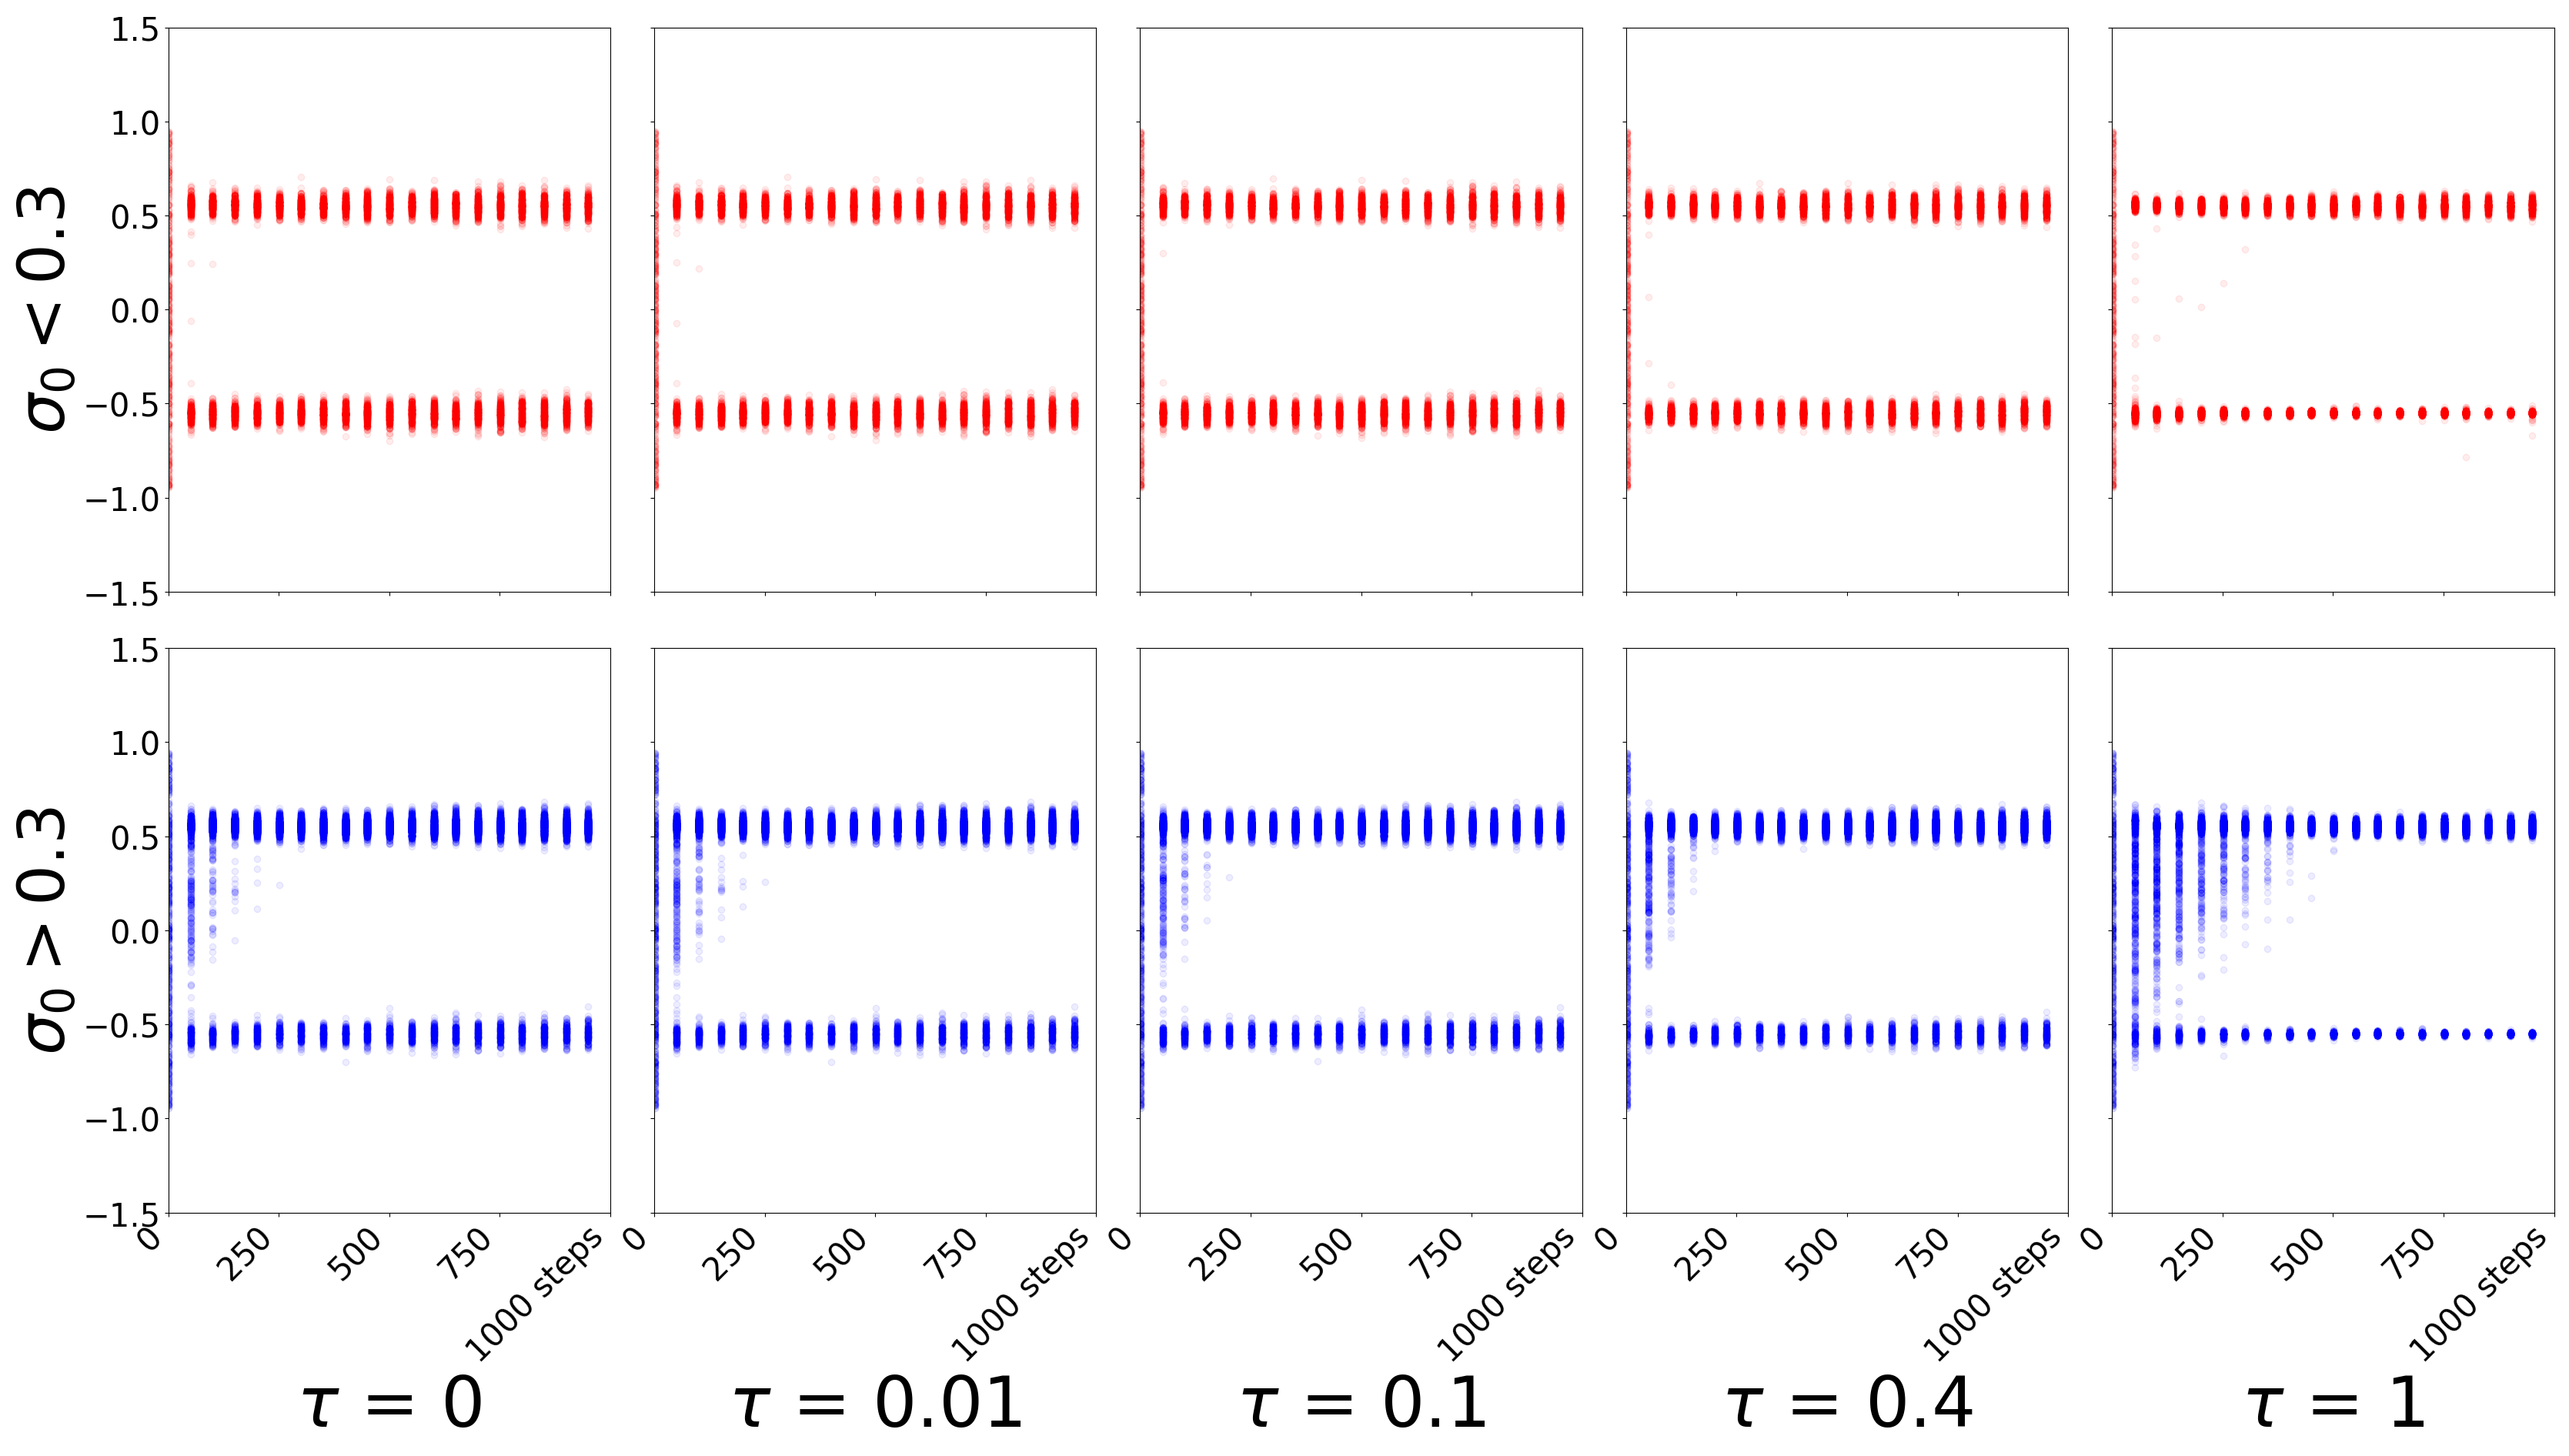
\includegraphics[width=\columnwidth]{figs/bandit/notlearnQ/modes=1/rmsprop/mean_reverse_optim=rmsprop_modes=1_lr=0.01.png}
    \caption{Reverse KL.}
    \label{fig:bandit-mean-reverse-rmsprop}
  \end{subfigure}
  \caption{Each plot tracks the mean over 1000 gradient steps of each of 1000 iterates. Each iterate is represented as a translucent, coloured dot with alpha value $0.01$. Temperature is varied on the $x$-major-axis and initial standard deviation $\sigma_0$ is varied on the $y$-major axis. Colour-coded by $\sigma_0$. Learning rate is 0.01.}
\end{figure}

\textbf{1)} FKL seems to facilitate more stable convergence of the iterates to the global optimum when $\sigma_0 > 0.3$. Indeed, outside of that setting, all iterates converge to a single optimum across all temperatures. 

\textbf{2)} Behaviour can vary across different standard deviation initializations. For $\tau < 0.4$, FKL iterates learn the optimal mode for all settings except when the $\sigma_0 < 0.3$. The achieved limit points of RKL iterates can differ depending on $\sigma_0$, such as with $\tau = 0.4$. 

\textbf{3)} RKL iterates converge to different local optima. The only case in which RKL iterates only converged to the optimal mode was for $\tau = 0.01$. 

\textbf{4)} At $\tau = 0.4$, FKL iterates converged to a point closer to zero than the RKL points, some of which remained at 0.5. This observation is consistent with our visualization of the loss surface, where the global optimum of the FKL loss moved to 0 more quickly than did the global optimum of the RKL loss. 
% 

These results are generally consistent with the FKL and RKL heatmaps, suggesting that for large enough $\sigma_0$, the FKL has a much smoother optimization landscape that directs iterates to the global minimum, but the global minimum might be suboptimal with respect to the original target distribution. One discrepancy with the visualization of the loss surfaces, however, is that both RKL and FKL exhibited limit points that do not appear to correspond to any optima on the heatmaps. In particular, FKL with $\sigma_0 < 0.3$ and $\tau \leq 0.1$ have iterates that stay in a neighbourhood away from 0, while the RKL at $\tau = 0.4$ and $\sigma_0 < 0.3$ has iterates that converge to 0. The same phenomenon was also present with both smaller and larger learning rates, and with RMSprop and SGD. While our initial surprise at the RKL limit point may be due to a limitation of our heatmaps--indeed, 0 might be a local minimum that is hard to distinguish amidst the dark area of \Cref{fig:bandit-heatmap}--the FKL limit point is more puzzling. The area around the line $\sigma = 0.3$ in \Cref{fig:bandit-heatmap} for $\tau = 0.01$ seems not to contain a local optimum. 

An earlier version of this experiment used integration points within the range $[-0.98, 0.98]$, rather than using all points but \{-1, 1\}. In this earlier setting, RKL iterates often diverged for $\sigma_0 > 0.3$ while FKL iterates maintained the same behaviour, suggesting that FKL is more robust to this type of bias than RKL. We comment more on the effect of numerical integration error in \Cref{sec:stochastic-microworld}. %Divergence of iterates in RKL occurs for larger $\sigma_0$, at $\tau = 0.01, 0.1$ where the iterates seem to fall into the suboptima at bottom corners of the heatmap. (Visualization of the gradients can be found in Appendix G)


\section{Switch-Stay}
Given our previous results, we might expect the FKL to perform better. If FKL iterates can reach the global optimum more easily, surely those policies would be better than policies updated under the RKL? One important factor, which we explore further below, is that the global minimum of the FKL objective may not correspond well with the optimal solution of the original, unregularized objective. 

We investigate the behavior of iterates when there is more than one state: the Switch-Stay environment. As a simple instantiation of the full RL problem, we are interested in understanding any possible differences between FKL and RKL in the presence of short-term/long-term trade-offs. In particular, on Switch-Stay, from state 0 one should incur a short-term penalty by switichng to state 1 to maximize return, given that $\gamma = 0.9$.

Another reason why we selected the Switch-Stay environment is for ease of visualization. Since the MDP has only two states, one can plot any value function as a point on a 2-dimensional plane. In particular, one can view the entire space of value functions, shown recently to be a polytope in the discrete-action setting \citep{dadashi2019value}. Plotting the value function corresponding to a policy as it changes over time allows us to view the progress of an algorithm and avoids the stochasticity inherent in performing rollouts and plotting learning curves.

To plot the boundary of the value function polytope in Switch-Stay, we plot the value functions corresponding to semi-deterministic policies (i.e., policies that are deterministic in at least one state) \citep{dadashi2019value}. Given a policy $\pi$, the value function $\vpi$ is calculated exactly as $(I - \gamma P_\pi)^{-1}r_\pi$, where $P_\pi$ and $r_\pi$ are respectively the transition matrix and the reward function induced by $\pi$. 

In the continuous version of switch-stay, we treat any action $ \leq 0$ as stay, and any action $ > 0$ as switch. To calculate the value function corresponding to a continuous policy $\pi$, we convert $\pi$ to an equivalent discrete policy $\pi_{\mathrm{discrete}}$ of the underlying discrete MDP. The conversion requires the calculation of the probability that $\pi$ outputs an action $\leq 0$ in each state, which we do with numerical integration of the policy PDF. We then calculate the value function of $\pi$ as $(I - \gamma P_{\pi_{\mathrm{discrete}}})^{-1}r_{\pi_{\mathrm{discrete}}}$.

For the hard FKL, we require access to the greedy action of the action-value function. In the continuous-action setting, this greedy action is usually infeasible to obtain. For the purposes of this experiment, if the greedy action is stay, we represent it in $[-1, 1]$ by drawing a uniform random number from $[-1, 0]$. If the greedy action is switch, we represent it as a uniform random number in $[0, 1]$. This design choice is meant to simulate noisy access to the greedy action in practice. 

As the policy is tabular in the states, we simply use the mean KL across states as the loss. 

\subsection{Behaviour}
% \paragraph{Optimization Path on Continuous Switch-Stay}
 %Based on our results for the bandit setting, we run three sets of experiments with three different standard deviation initializations, such that $\sigma_0$ is in $(0.1, 0.3), (0.3, 1)$. 
For all of these experiments, we initialized means in the range $(-0.95, 0.95)$. All experiments are run for 500 gradient steps and each experiment has 1000 iterates. We plot the value function of the final policy for each iterate and experiment in \Cref{fig:cont-ss-poly-0.005,fig:cont-ss-poly-0.01}, by visualizing the value function polytope \citep{dadashi2019value}. 


% \begin{figure}[!htb]
%   \centering
%   \begin{subfigure}[b]{0.7\linewidth}
%     \centering
%     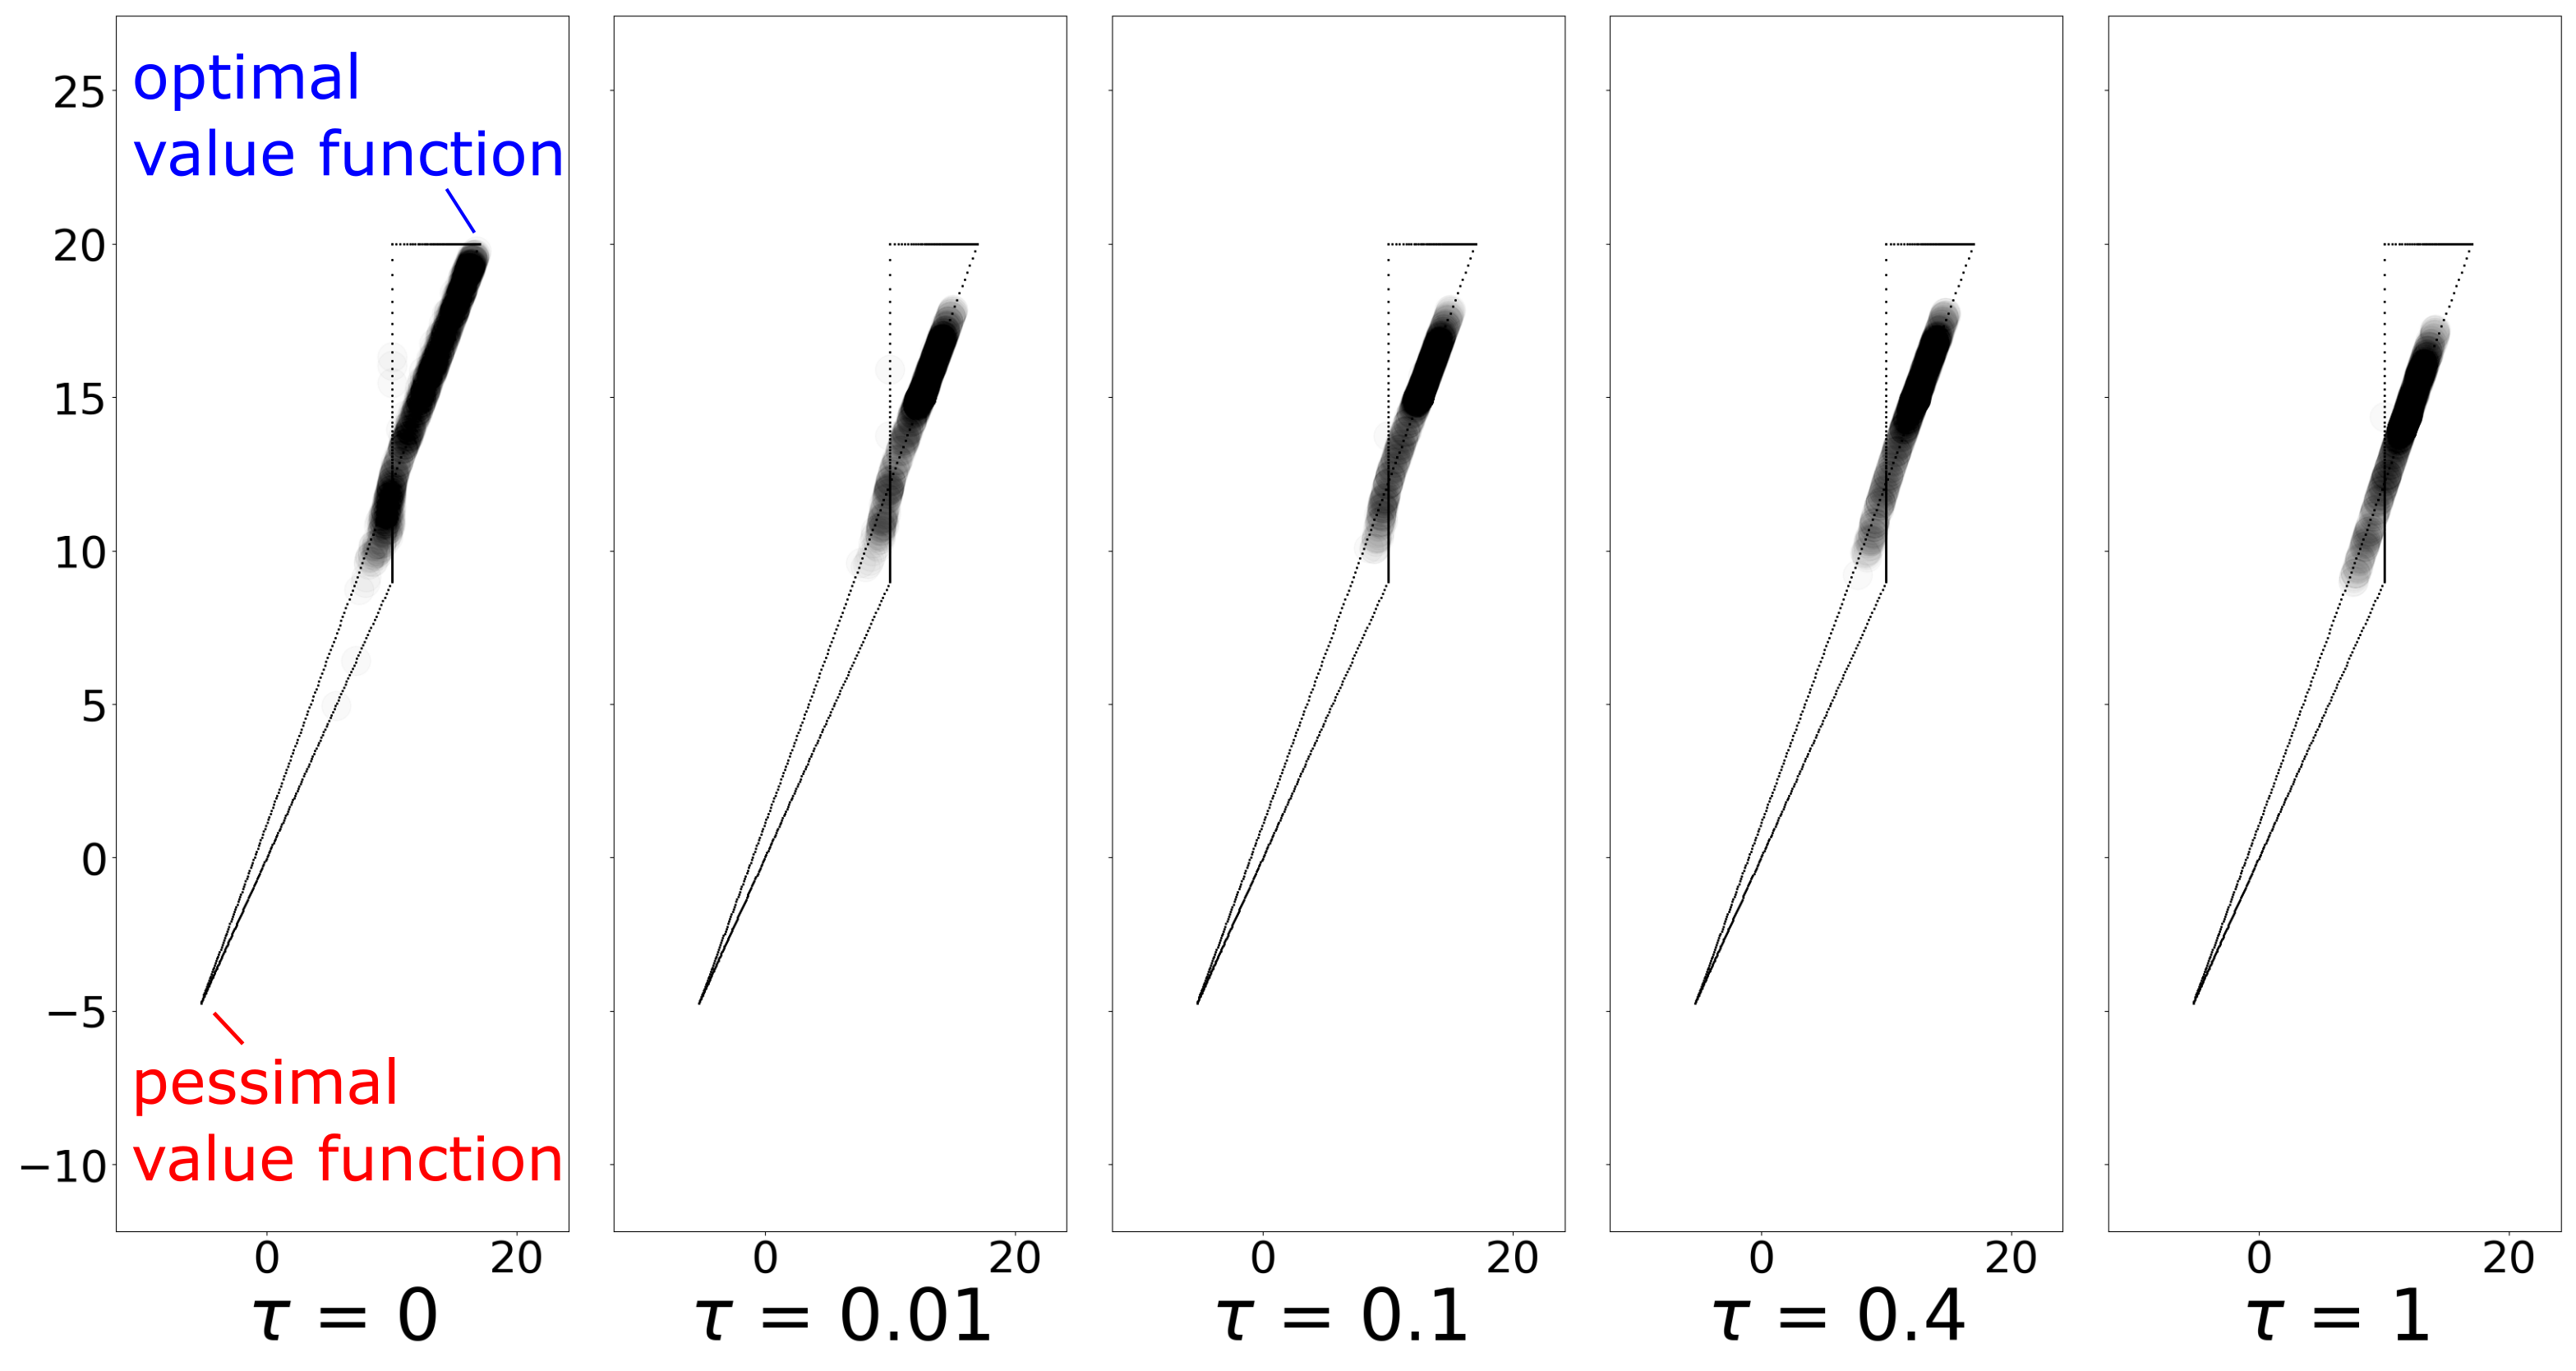
\includegraphics[width=\columnwidth]{figs/continuous-switch-stay/notlearnQ/cont_poly.png}
%     \caption{Forward KL, learning rate = $0.005$.}
%     \label{fig:cont-switch-stay-forward}
%   \end{subfigure}\hspace{15pt}
  
%   \begin{subfigure}[b]{0.7\linewidth}
%         \centering
%         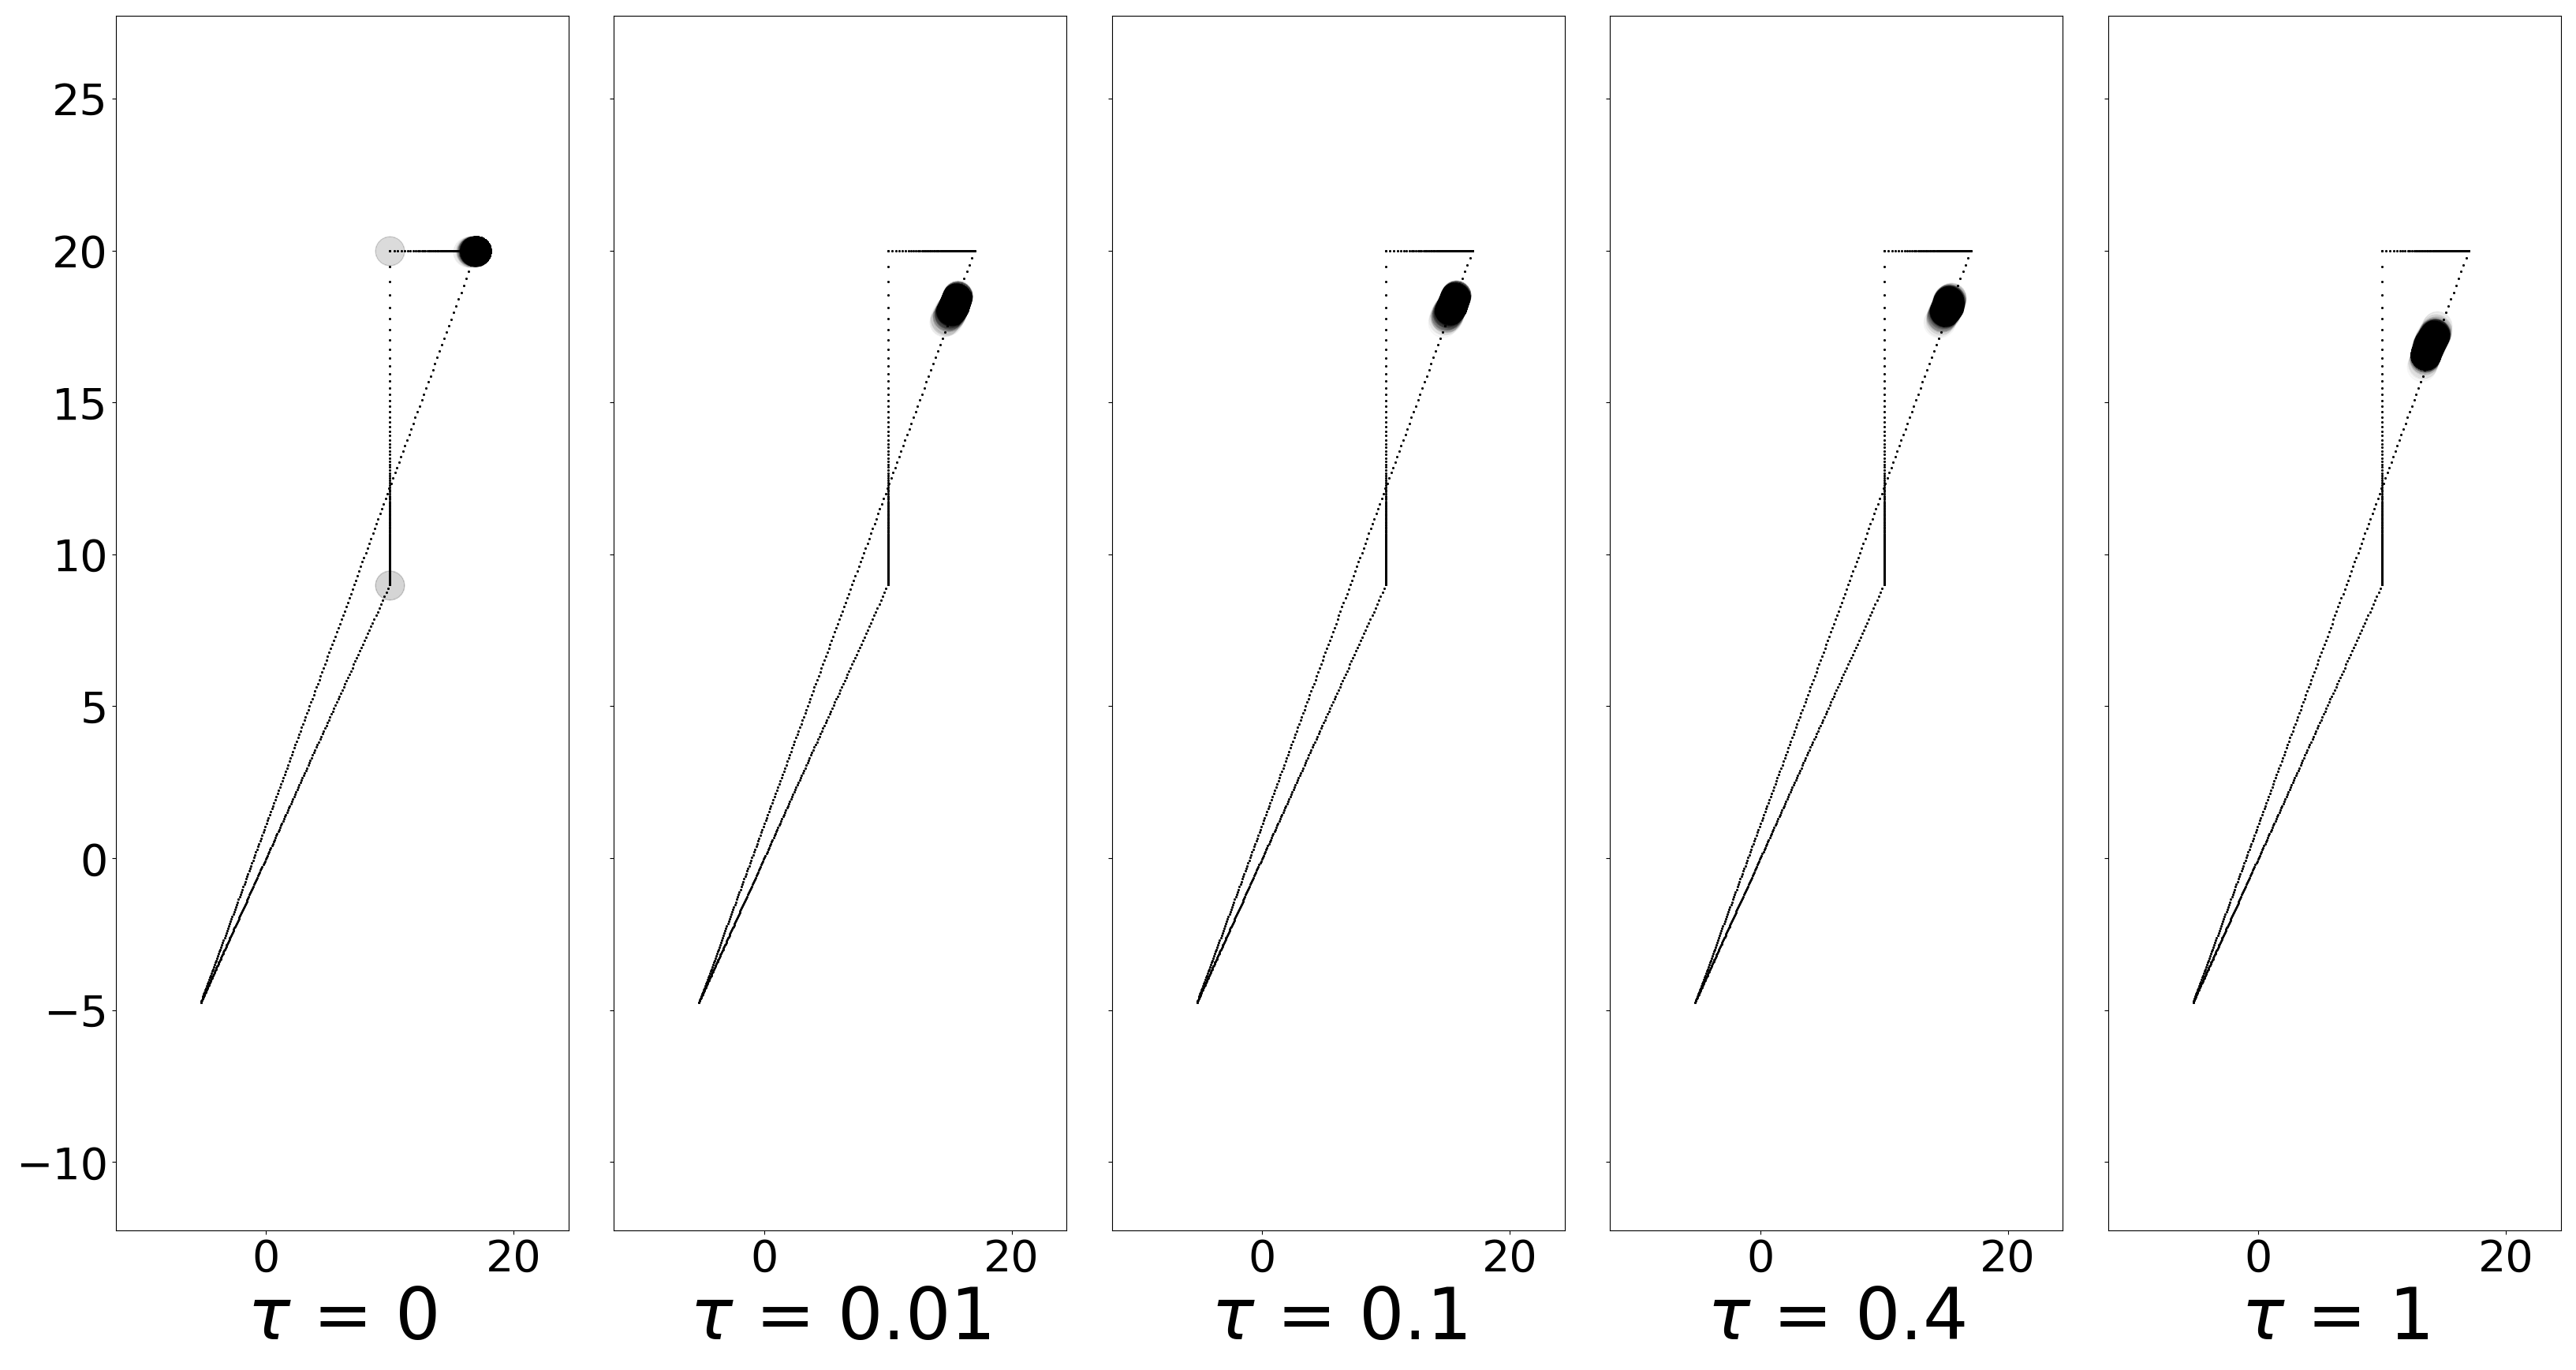
\includegraphics[width=\columnwidth]{figs/continuous-switch-stay/notlearnQ/polytope_reverse_optim=adam_lr=0.005.png}
%         \caption{Reverse KL, learning rate = $0.005$.}
%         \label{fig:cont-switch-stay-reverse}
%   \end{subfigure}
%   \caption{Each subplot plots the final value functions on the continuous version of switch-stay after 500 gradient steps with $\gamma = 0.9$ for 1000 iterates. Each iterate is represented by a translucent dot with alpha value $0.01$. Using Adam. Temperature is varied on the $x$-major-axis.}
%   \label{fig:cont-ss-poly-0.005}
% \end{figure}

\begin{figure}[!htb]
  \centering
  \begin{subfigure}[b]{0.7\linewidth}
    \centering
    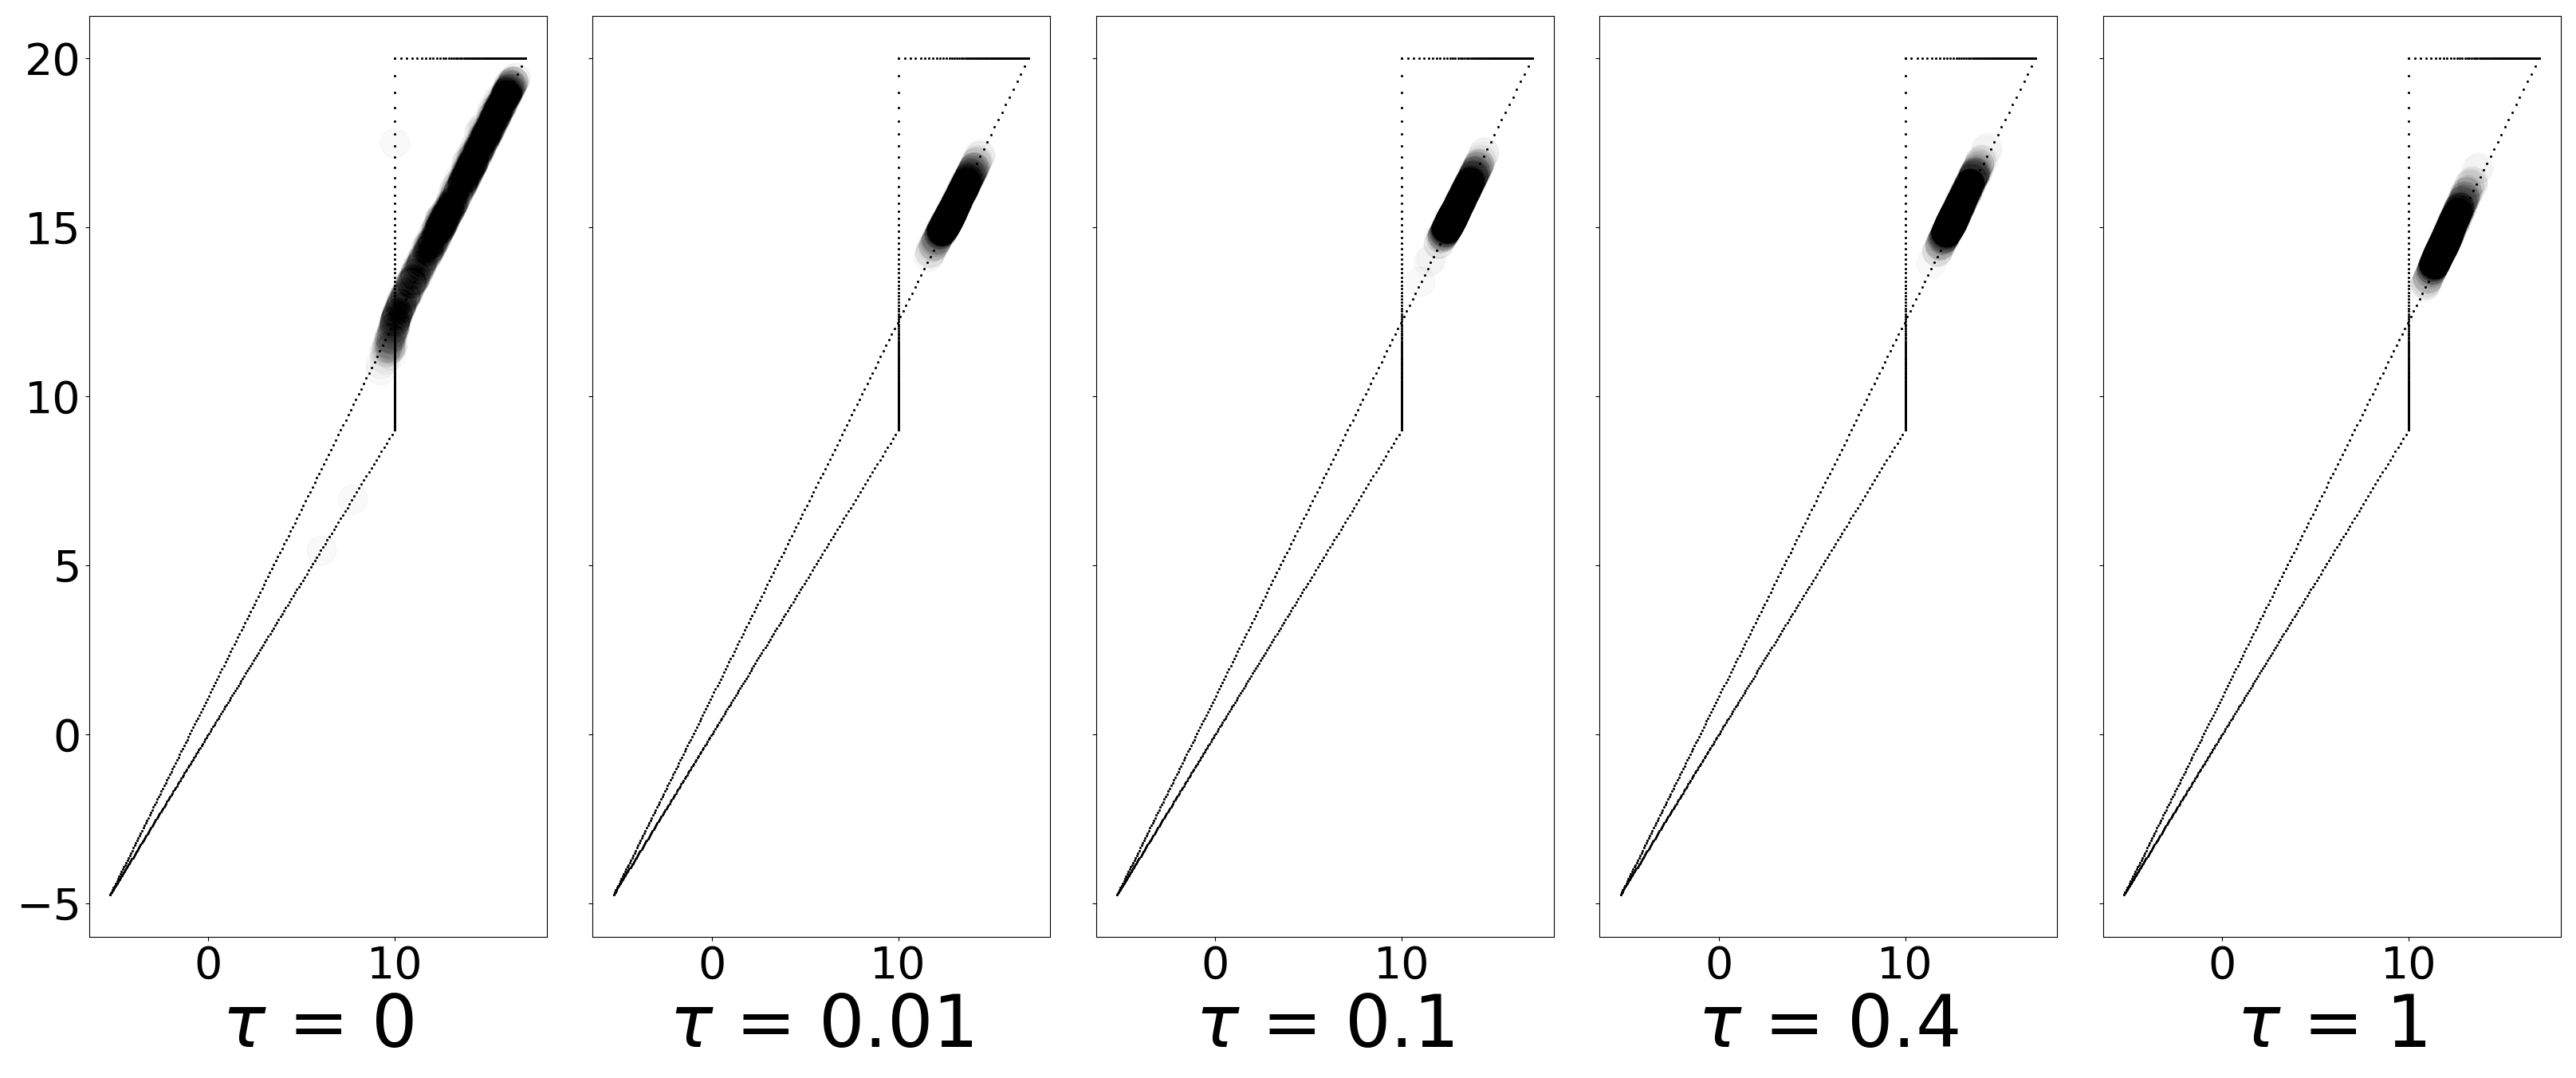
\includegraphics[width=\columnwidth]{figs/continuous-switch-stay/notlearnQ/polytope_forward_optim=rmsprop_lr=0.005.png}
    \caption{Forward KL, learning rate = $0.005$.}
    \label{fig:cont-switch-stay-forward}
  \end{subfigure}\hspace{15pt}
  
  \begin{subfigure}[b]{0.7\linewidth}
        \centering
        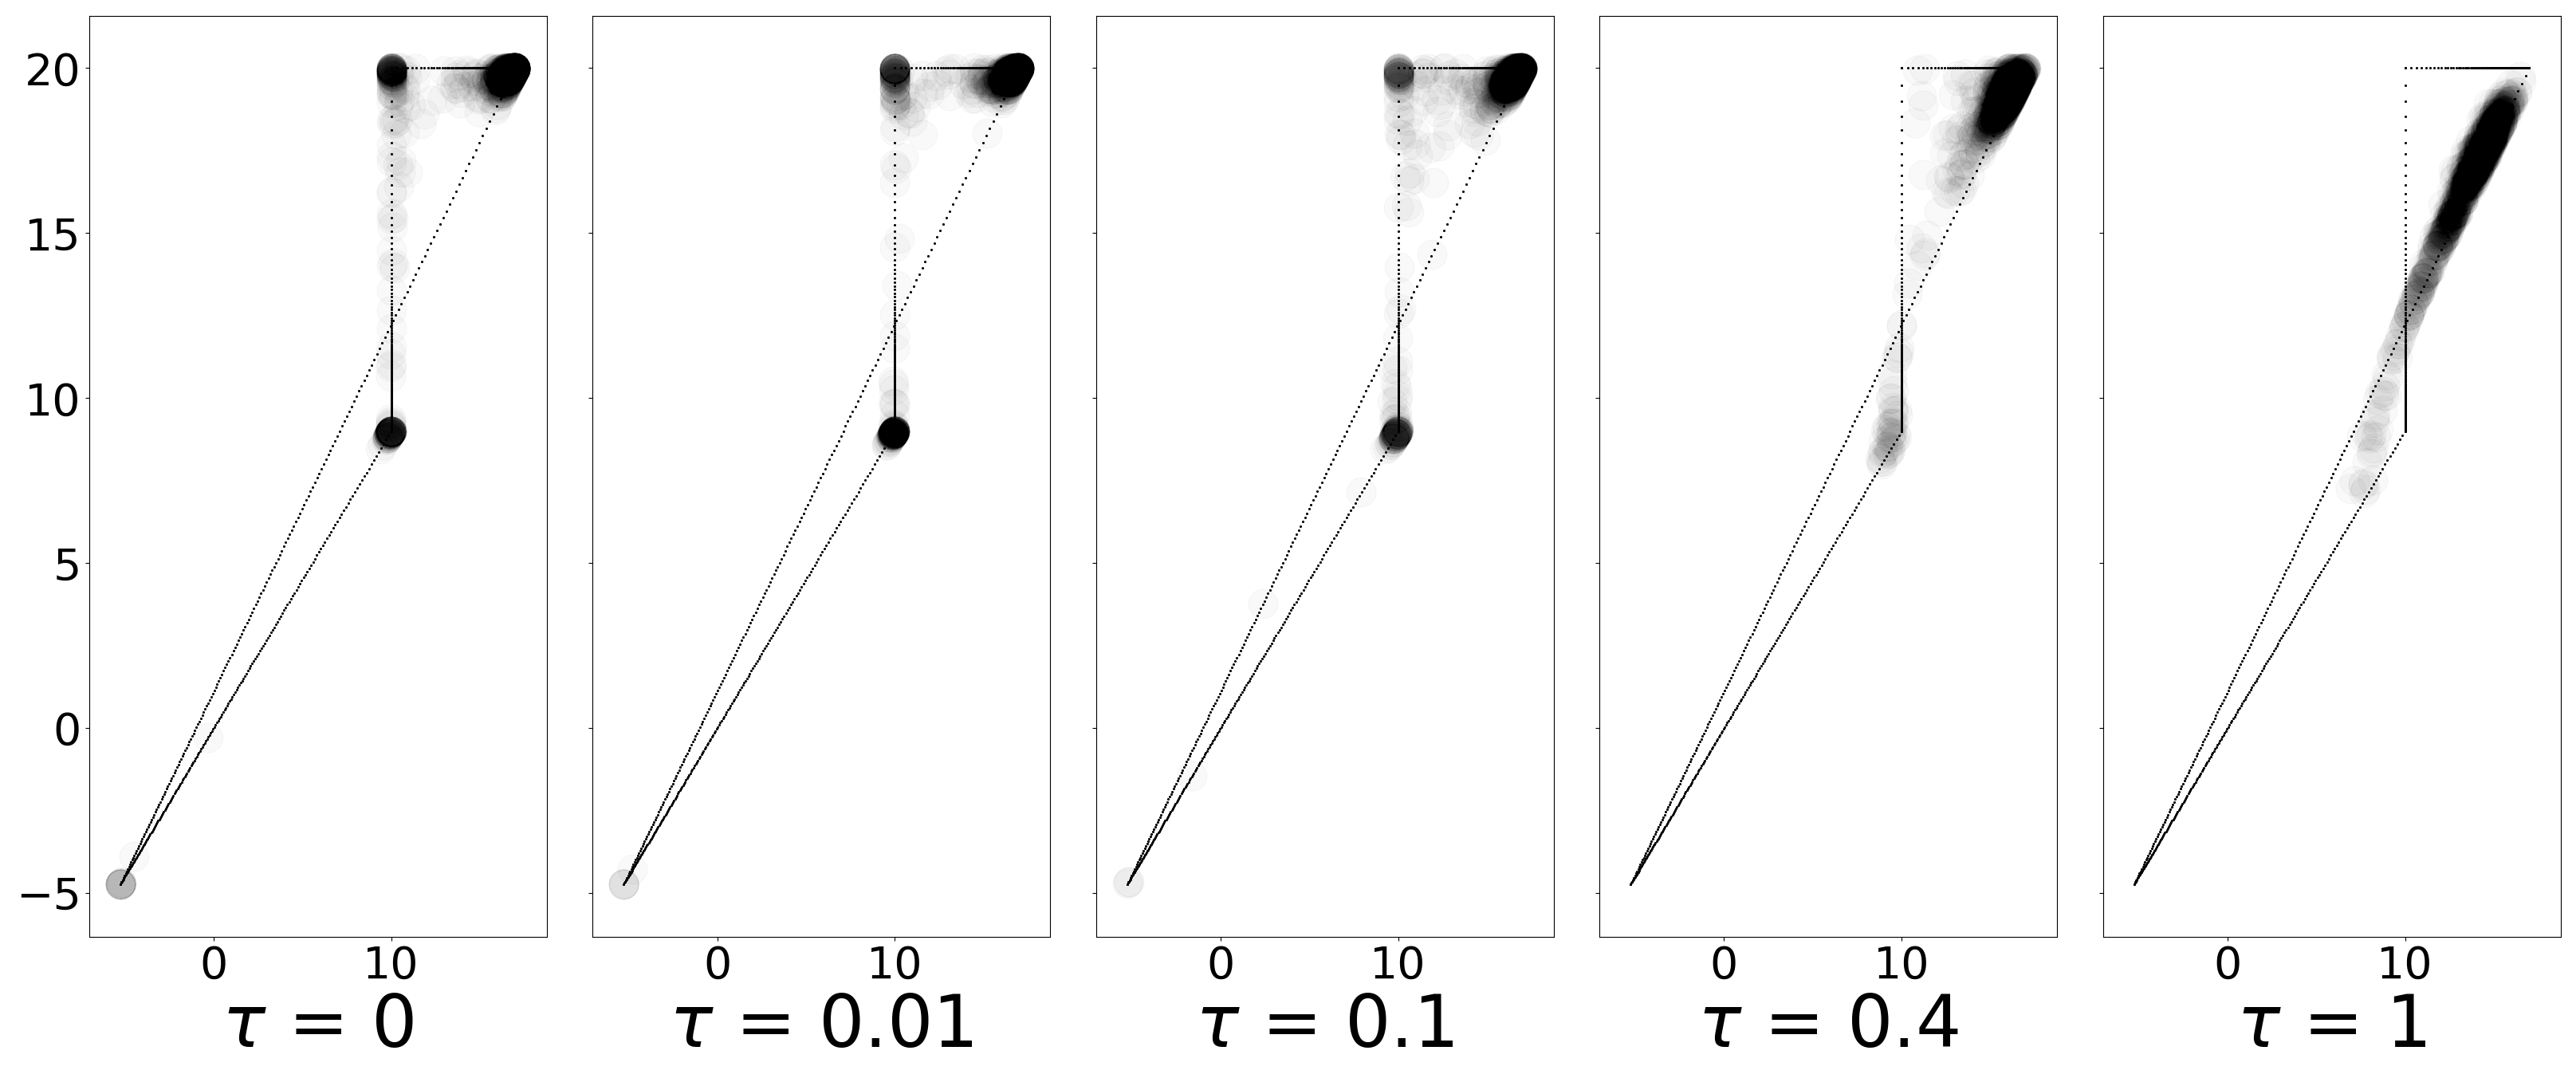
\includegraphics[width=\columnwidth]{figs/continuous-switch-stay/notlearnQ/polytope_reverse_optim=rmsprop_lr=0.005.png}
        \caption{Reverse KL, learning rate = $0.005$.}
        \label{fig:cont-switch-stay-reverse}
  \end{subfigure}
  \caption{Each subplot plots the final value functions on the continuous version of switch-stay after 500 gradient steps with $\gamma = 0.9$ for 1000 iterates. The top-right corner of the polytope in each subplot is the optimal value function and the bottom-left corner is the pessimal value function. Each iterate is represented by a translucent dot with alpha value $0.01$. Using RMSprop. Temperature is varied on the $x$-major-axis.}
  \label{fig:cont-ss-poly-0.005}
\end{figure}

% \begin{figure}[!htb]
%     \centering
%     \begin{subfigure}{0.7\linewidth}
%     \centering
%     \includegraphics[width=\columnwidth]{figs/continuous-switch-stay/notlearnQ/polytope_forward_optim=adam_lr=0.01.png}
%     \caption{Forward KL, learning rate = $0.01$.}
%     \label{fig:cont-switch-stay-forward-0.01}
%   \end{subfigure}\hspace{15pt}
  
%   \begin{subfigure}[b]{0.7\linewidth}
%         \centering
%         \includegraphics[width=\columnwidth]{figs/continuous-switch-stay/notlearnQ/polytope_reverse_optim=adam_lr=0.01.png}
%         \caption{Reverse KL, learning rate = $0.01$.}
%         \label{fig:cont-switch-stay-reverse-0.01}
%   \end{subfigure}
%   \caption{See \Cref{fig:cont-ss-poly-0.005}.}
%   \label{fig:cont-ss-poly-0.01}
% \end{figure}

\begin{figure}[!htb]
    \centering
    \begin{subfigure}{0.7\linewidth}
    \centering
    \includegraphics[width=\columnwidth]{figs/continuous-switch-stay/notlearnQ/polytope_forward_optim=rmsprop_lr=0.01.png}
    \caption{Forward KL, learning rate = $0.01$.}
    \label{fig:cont-switch-stay-forward-0.01}
  \end{subfigure}\hspace{15pt}
  
  \begin{subfigure}[b]{0.7\linewidth}
        \centering
        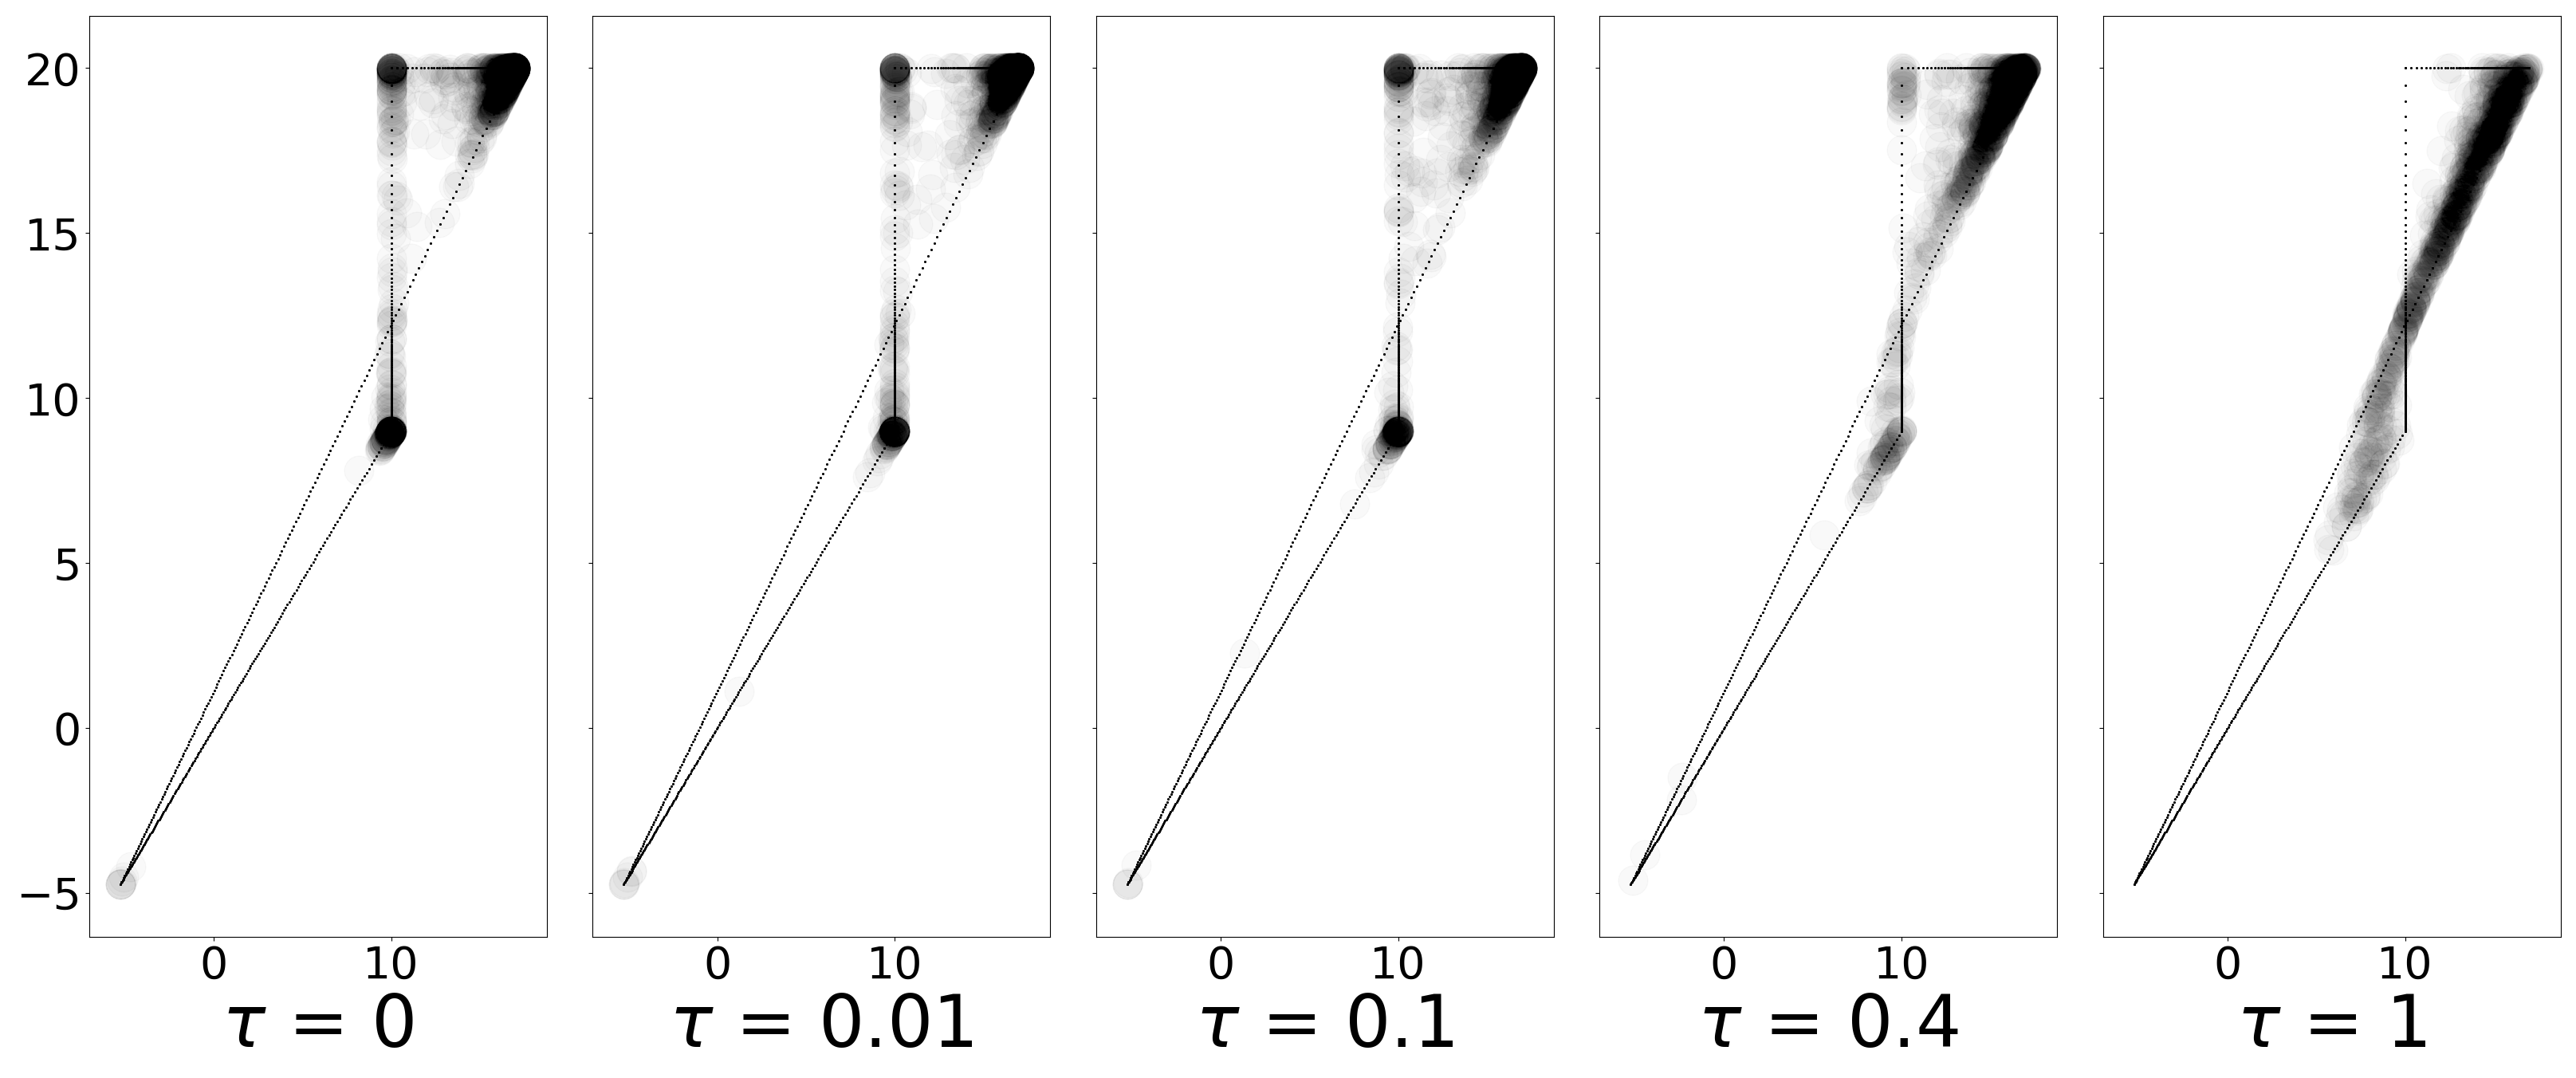
\includegraphics[width=\columnwidth]{figs/continuous-switch-stay/notlearnQ/polytope_reverse_optim=rmsprop_lr=0.01.png}
        \caption{Reverse KL, learning rate = $0.01$.}
        \label{fig:cont-switch-stay-reverse-0.01}
  \end{subfigure}
  \caption{See \Cref{fig:cont-ss-poly-0.005}.}
  \label{fig:cont-ss-poly-0.01}
\end{figure}

\textbf{1)} FKL with $\tau = 0$ converged noticeably slower than the other temperatures, which seems to be an artifact of our encoding of continuous actions to the underlying discrete dynamics of switch-stay, and the fact that we used random tie-breaking when computing the $\argmax$ for hard FKL. 

\textbf{2)} RKL iterates converge slightly faster than FKL iterates across all temperature settings. RKL iterates with $\tau = 0$ sometimes converged to non-optimal value functions on the corners. 

\textbf{3)} The limiting value functions of the FKL iterates seem more suboptimal than the limiting value functions of the RKL iterates; the latter are closer to the optimal value function of the original MDP. This result is consistent with our observations in the continuous bandit; although the FKL optimum may be more easily reached, that optimal point may be suboptimal with respect to an ``original'' objective (in this case, the optimal value function of the unregularized MDP). 

To further our understanding of \textbf{3)}, we plot the final means and standard deviations of the learned policies for the learning rate of 0.01. In \Cref{fig:final-ss-probs-0,fig:final-ss-probs-1}, we see that the final FKL iterates have higher standard deviation, meaning that the final policies are further from the optimal deterministic policy of the unregularized MDP. Put informally, the FKL tends to ``commit'' less than the RKL.  

In \Cref{fig:final-ss-probs-0,fig:final-ss-probs-1} as well, we note that the spread of the final iterates is much larger for the leftmost column, representing $\tau = 0$, than for any of the other columns. This spread is consistent with the spread observed in the leftmost columns of \Cref{fig:cont-ss-poly-0.005,fig:cont-ss-poly-0.01}. For the RKL, this spread seems to be a representation of the local minima. For the FKL, this result is likely an artifact of our encoding of the maximum action as a uniform random point in either [0, 1] or [-1, 0], depending on if the maximum action is respectively stay or switch. 

% \begin{figure}[!htb]
%   \centering
%   \begin{subfigure}[b]{0.85\linewidth}
%     \centering
%     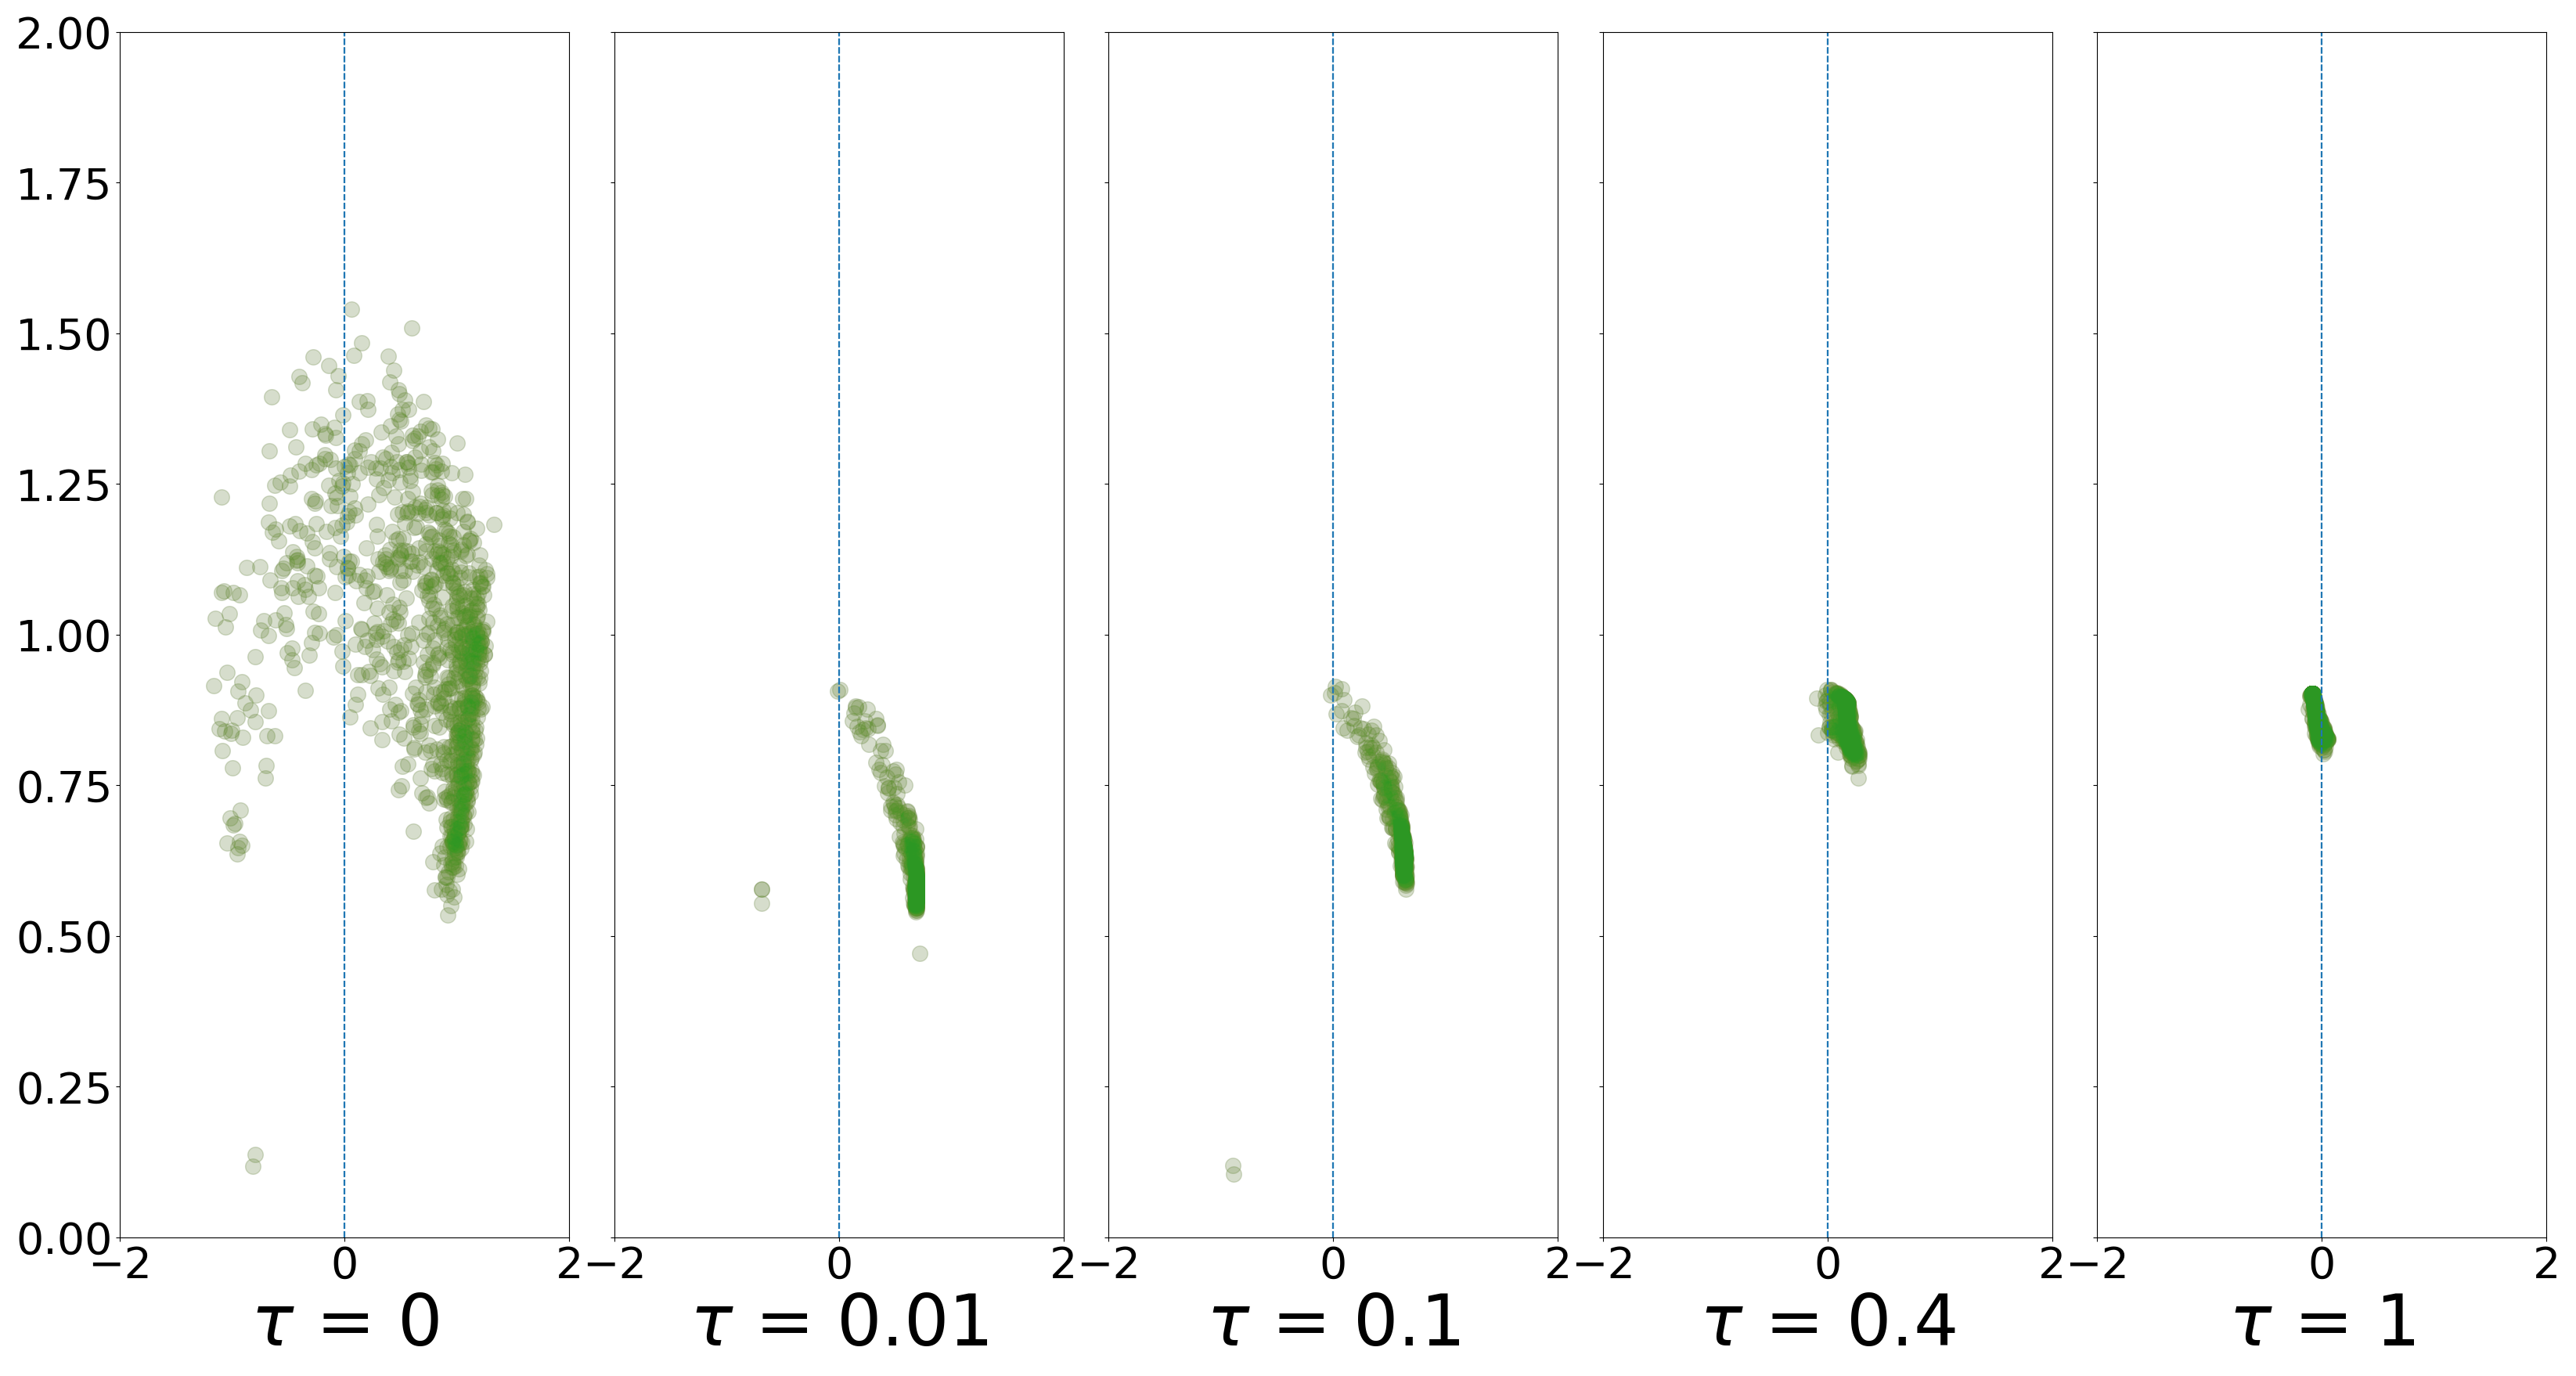
\includegraphics[width=\columnwidth]{figs/continuous-switch-stay/notlearnQ/state0_pi_forward_optim=adam_lr=0.01.png}
%     \caption{Forward KL on state 0.}
%     \label{fig:cont-switch-stay-forward-s0}
%   \end{subfigure}\hspace{15pt}
  
%   \begin{subfigure}[b]{0.85\linewidth}
%         \centering
%         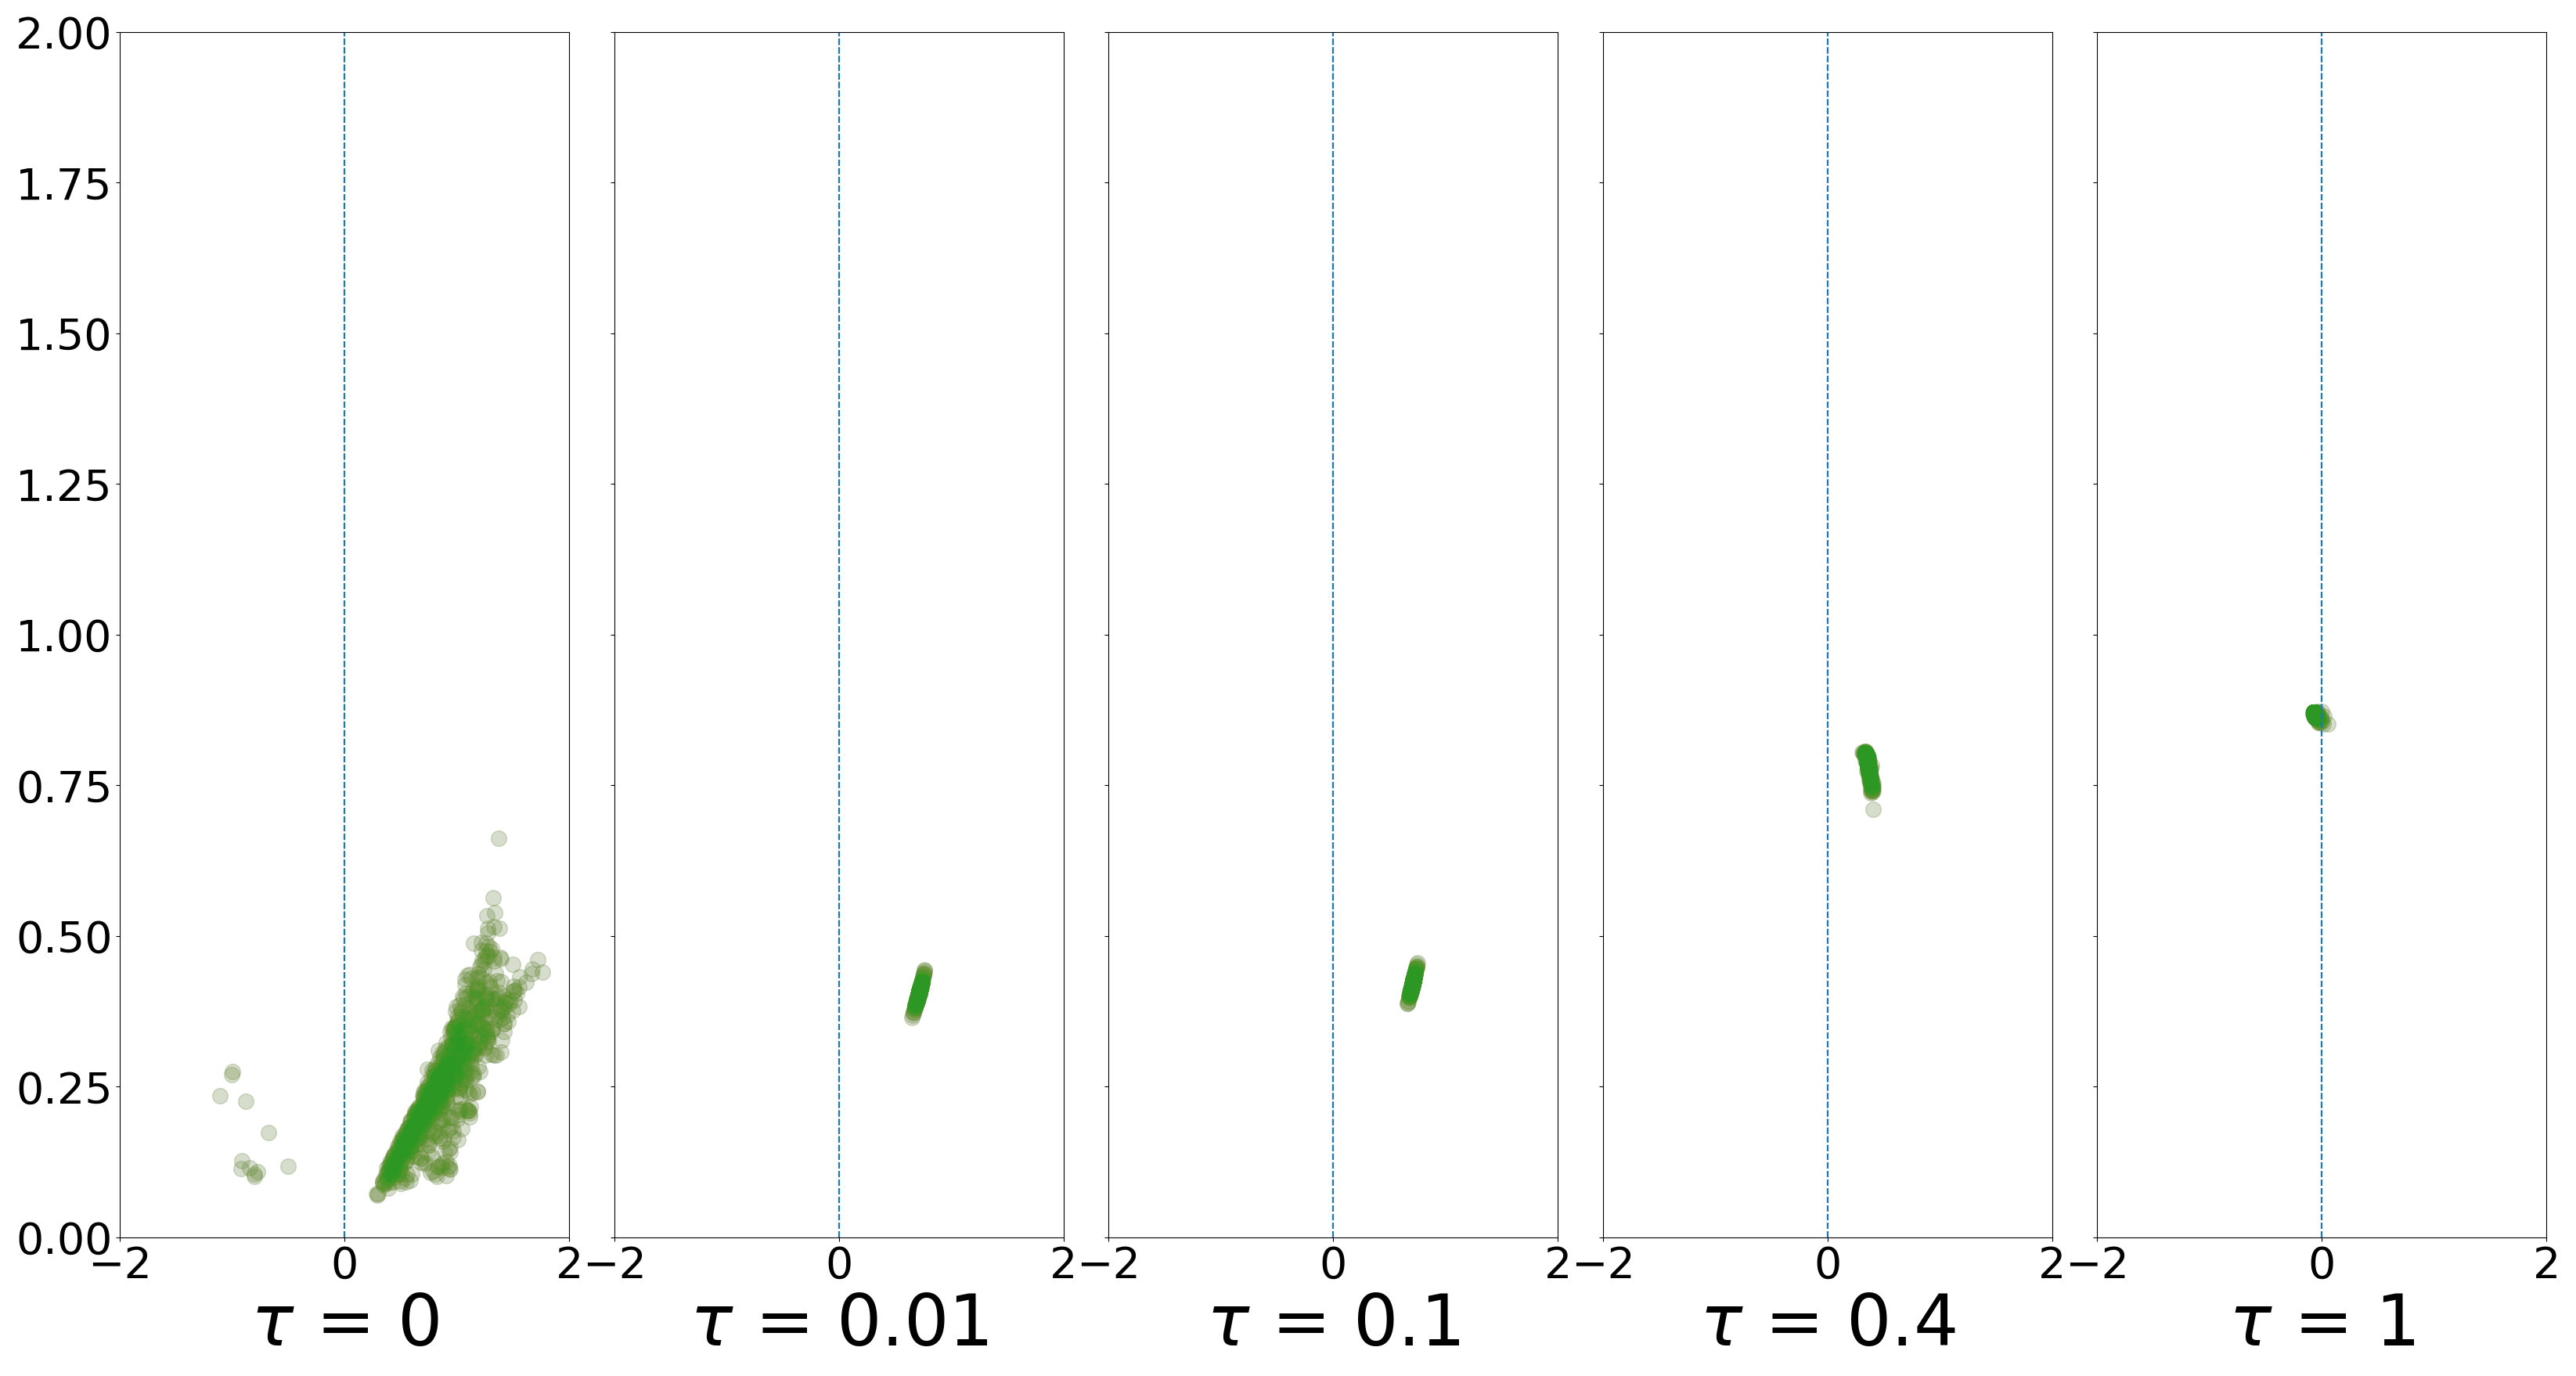
\includegraphics[width=\columnwidth]{figs/continuous-switch-stay/notlearnQ/state0_pi_reverse_optim=adam_lr=0.01.png}
%         \caption{Reverse KL on state 0.}
%         \label{fig:cont-switch-stay-reverse-s0}
%   \end{subfigure}

%   \caption{Each subplot plots the final mean (x-axis) and standard deviation (y-axis) on the continuous version of switch-stay after 500 gradient steps with $\gamma = 0.9$ for 1000 iterates. Each iterate is represented by a translucent dot with alpha value $0.1$. Using Adam with learning rate $0.01$. Temperature is varied on the $x$-major-axis. Every action $\leq 0$ is treated as ``stay'' and every action $> 0$ is treated as ``switch''. The blue dotted line in subplots corresponds to the line $\mu = 0$. }
%   \label{fig:final-ss-probs-0}
% \end{figure}

\begin{figure}[!htb]
  \centering
  \begin{subfigure}[b]{0.85\linewidth}
    \centering
    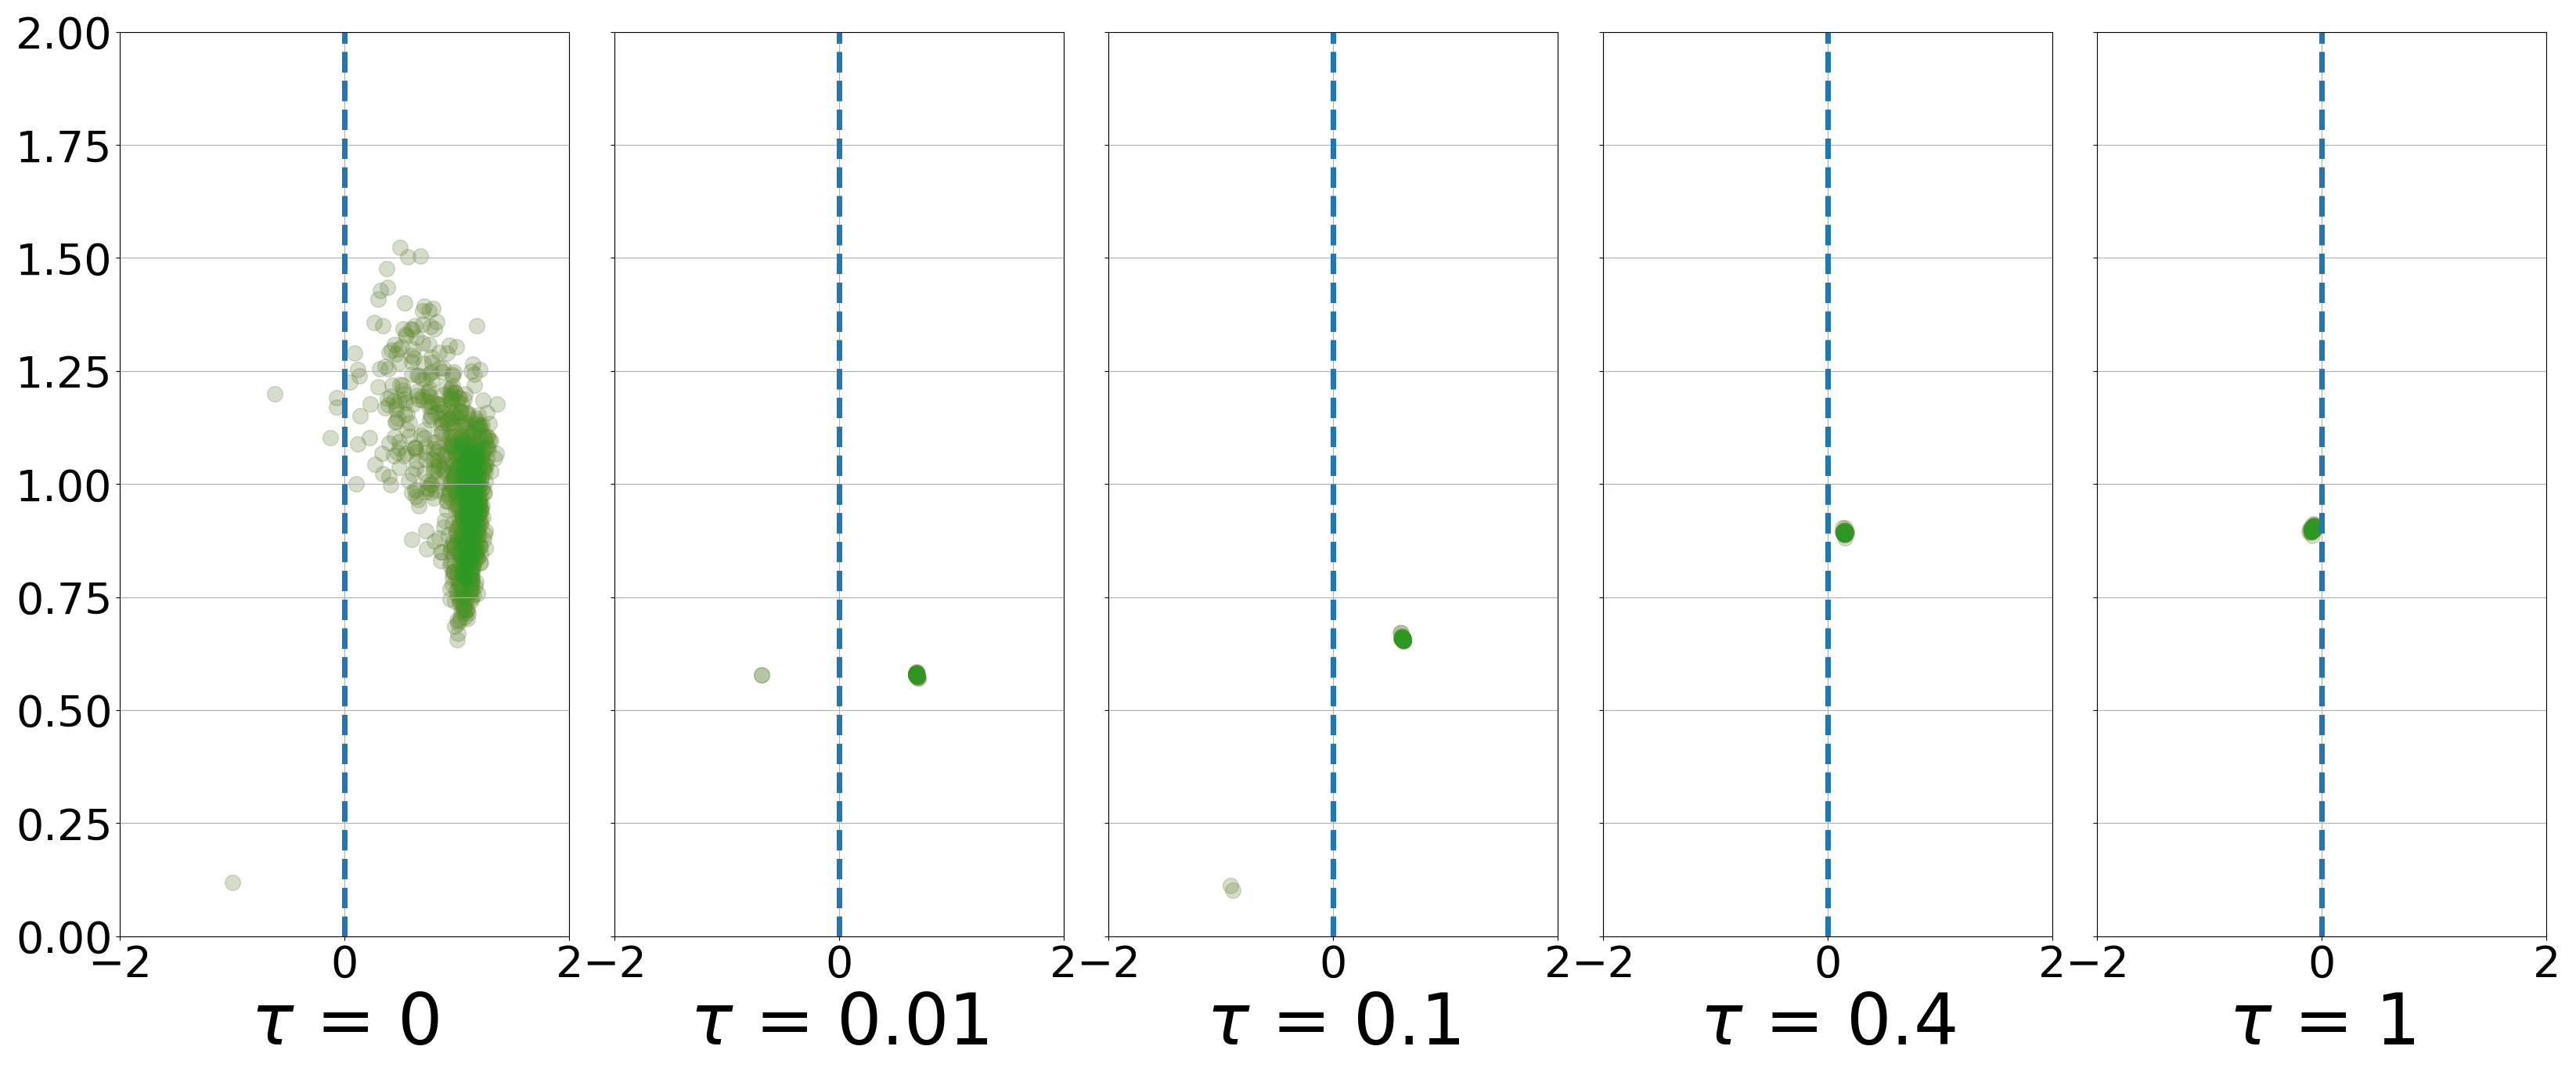
\includegraphics[width=\columnwidth]{figs/continuous-switch-stay/notlearnQ/state0_pi_forward_optim=rmsprop_lr=0.01.png}
    \caption{Forward KL on state 0.}
    \label{fig:cont-switch-stay-forward-s0}
  \end{subfigure}\hspace{15pt}
  
  \begin{subfigure}[b]{0.85\linewidth}
        \centering
        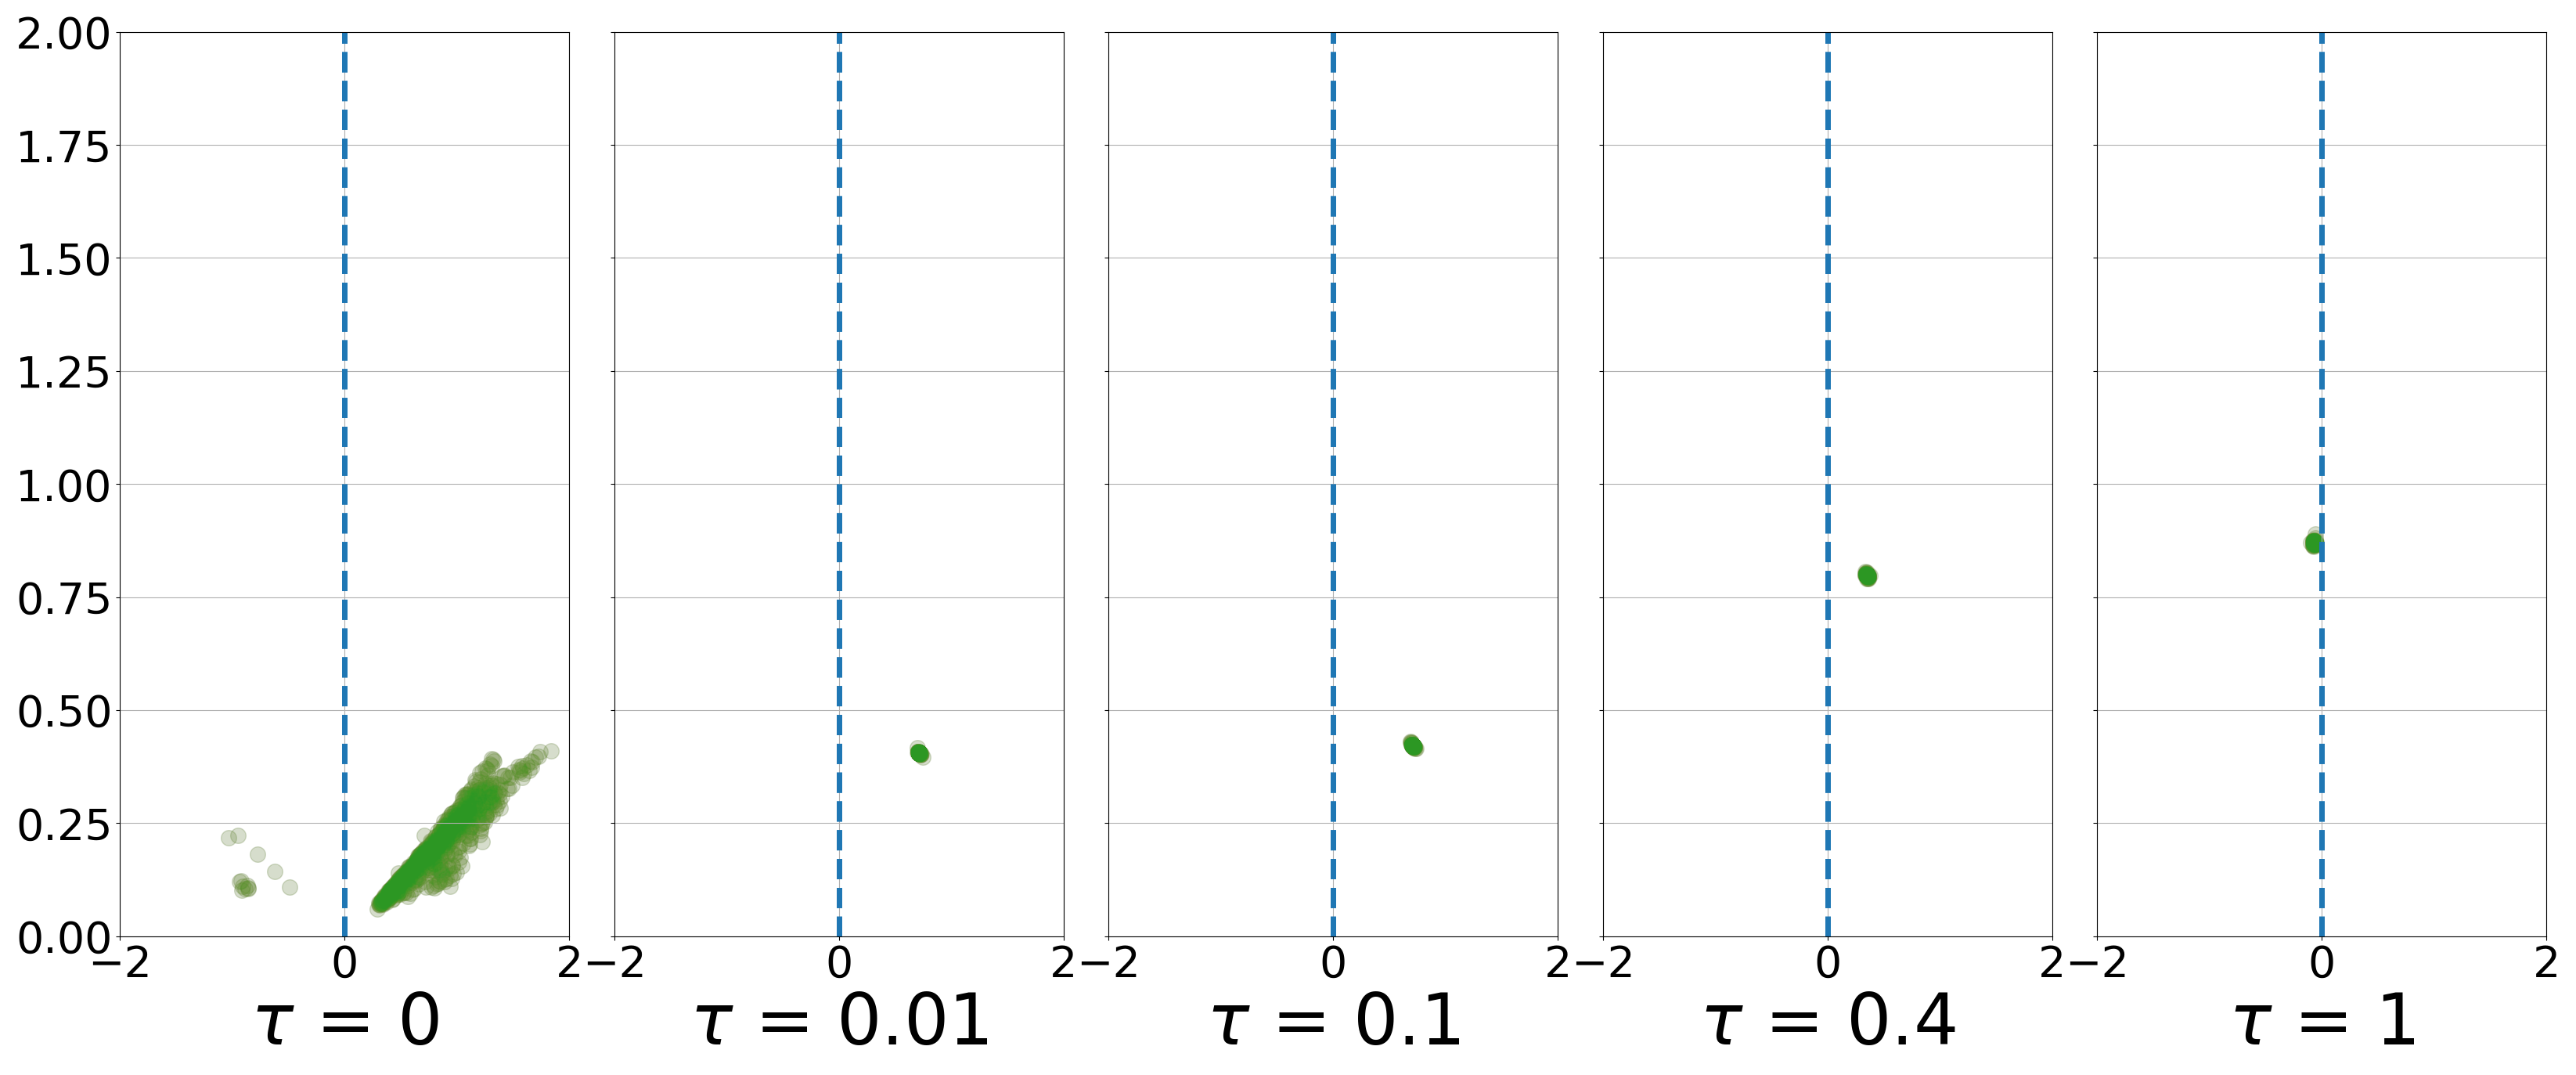
\includegraphics[width=\columnwidth]{figs/continuous-switch-stay/notlearnQ/state0_pi_reverse_optim=rmsprop_lr=0.01.png}
        \caption{Reverse KL on state 0.}
        \label{fig:cont-switch-stay-reverse-s0}
  \end{subfigure}

  \caption{Each subplot plots the final mean (x-axis) and standard deviation (y-axis) on the continuous version of switch-stay after 500 gradient steps with $\gamma = 0.9$ for 1000 iterates. Each iterate is represented by a translucent dot with alpha value $0.1$. Using RMSprop with learning rate $0.01$. Temperature is varied on the $x$-major-axis. Every action $\leq 0$ is treated as ``stay'' and every action $> 0$ is treated as ``switch''. The blue dotted line in subplots corresponds to the line $\mu = 0$. }
  \label{fig:final-ss-probs-0}
\end{figure}

% \begin{figure}[!htb]
% \centering
% \begin{subfigure}[b]{0.85\linewidth}
%     \centering
%     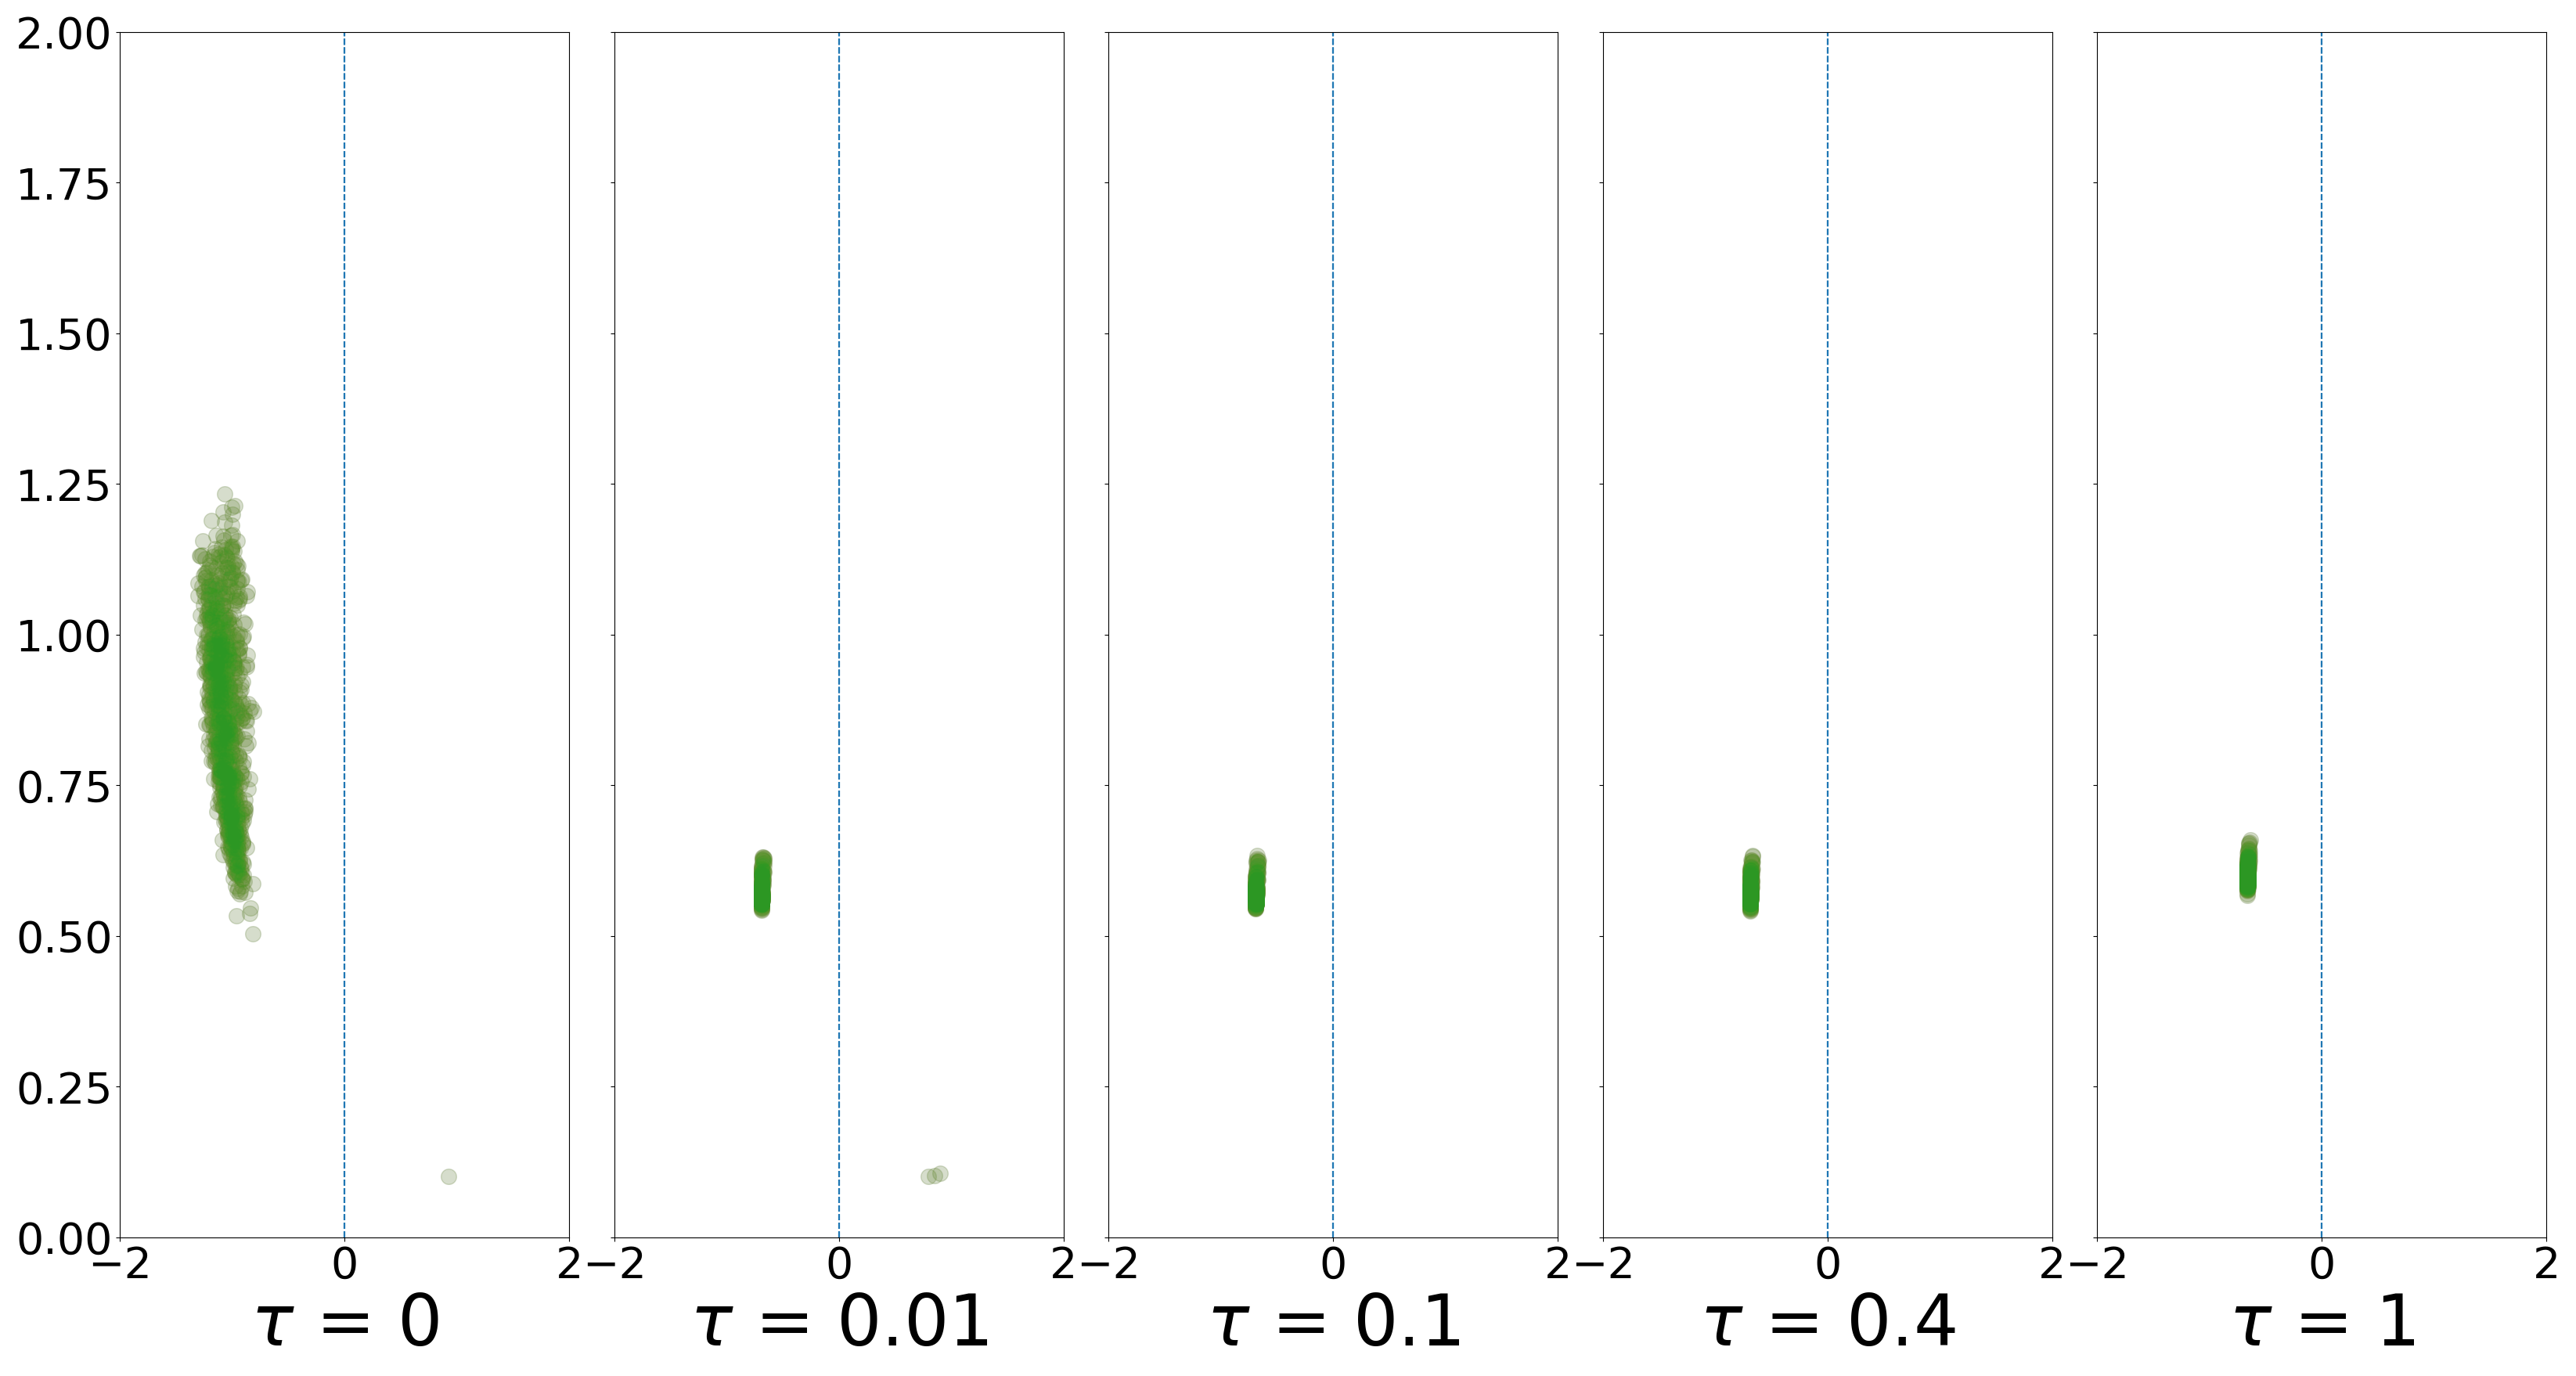
\includegraphics[width=\columnwidth]{figs/continuous-switch-stay/notlearnQ/state1_pi_forward_optim=adam_lr=0.01.png}
%     \caption{Forward KL on state 1.}
%     \label{fig:cont-switch-stay-forward-s1}
%   \end{subfigure}\hspace{15pt}
  
%   \begin{subfigure}[b]{0.85\linewidth}
%         \centering
%         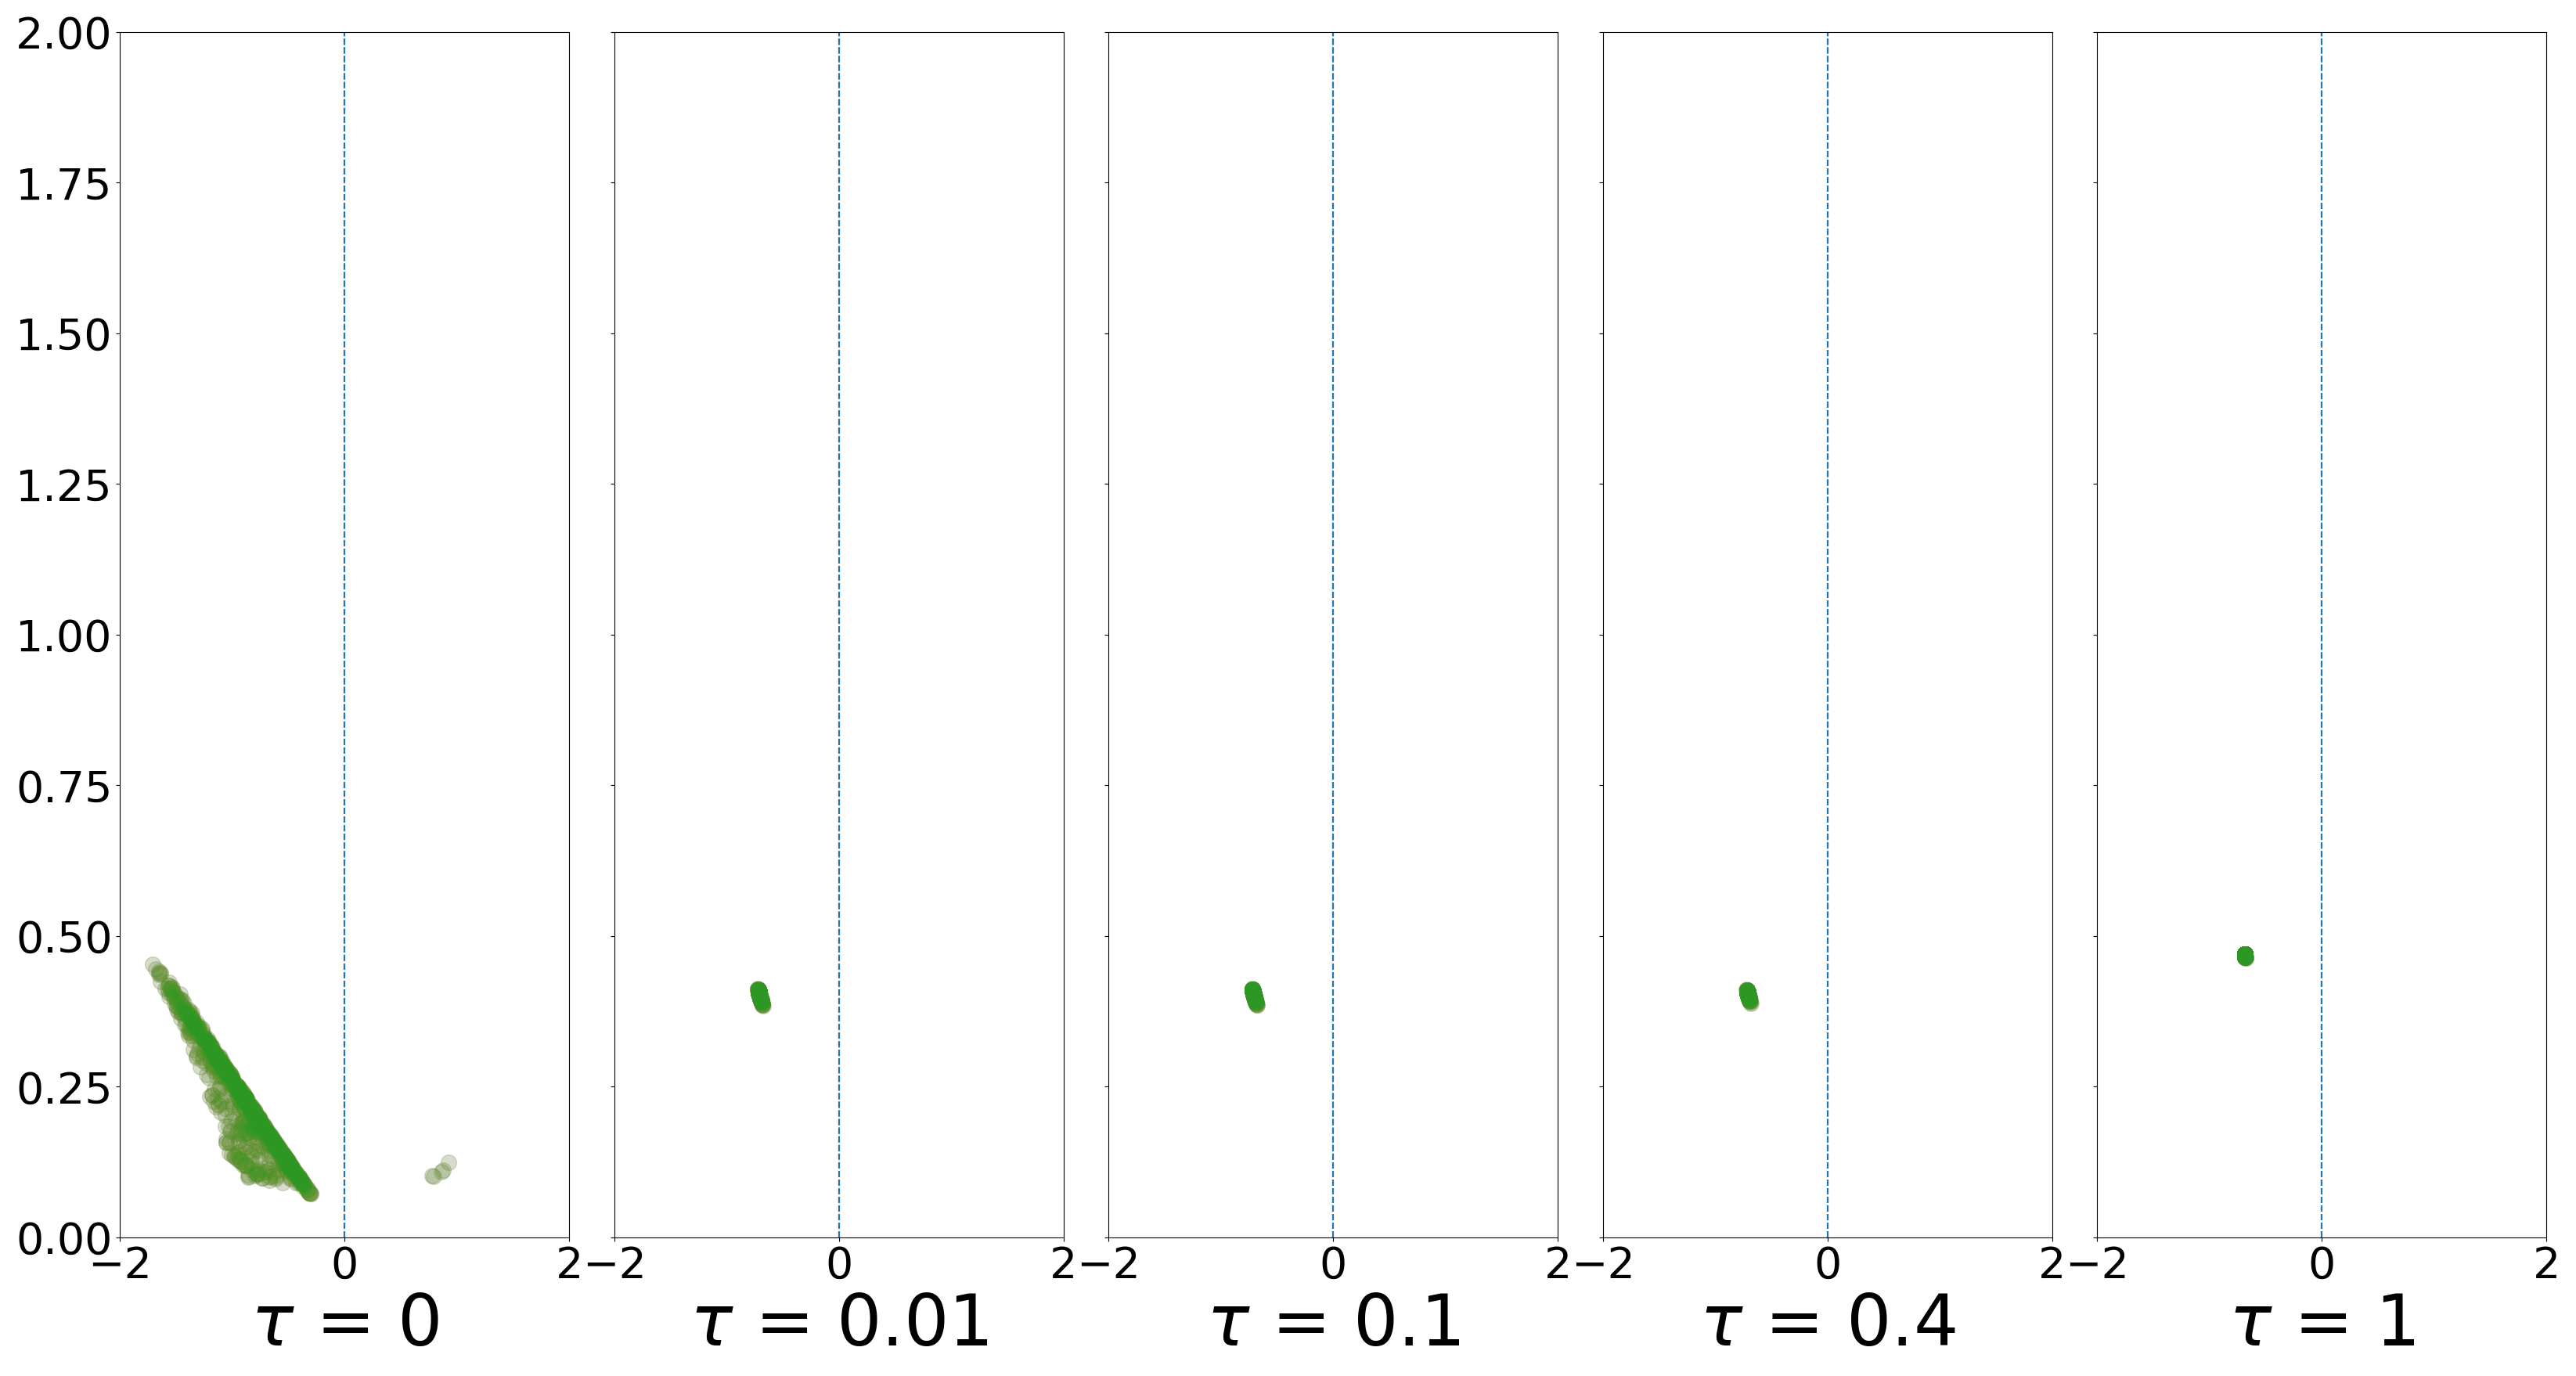
\includegraphics[width=\columnwidth]{figs/continuous-switch-stay/notlearnQ/state1_pi_reverse_optim=adam_lr=0.01.png}
%         \caption{Reverse KL on state 1.}
%         \label{fig:cont-switch-stay-reverse-s1}
%   \end{subfigure}
%   \caption{See \Cref{fig:final-ss-probs-0}.}
%   \label{fig:final-ss-probs-1}
% \end{figure}


\begin{figure}[!htb]
\centering
\begin{subfigure}[b]{0.85\linewidth}
    \centering
    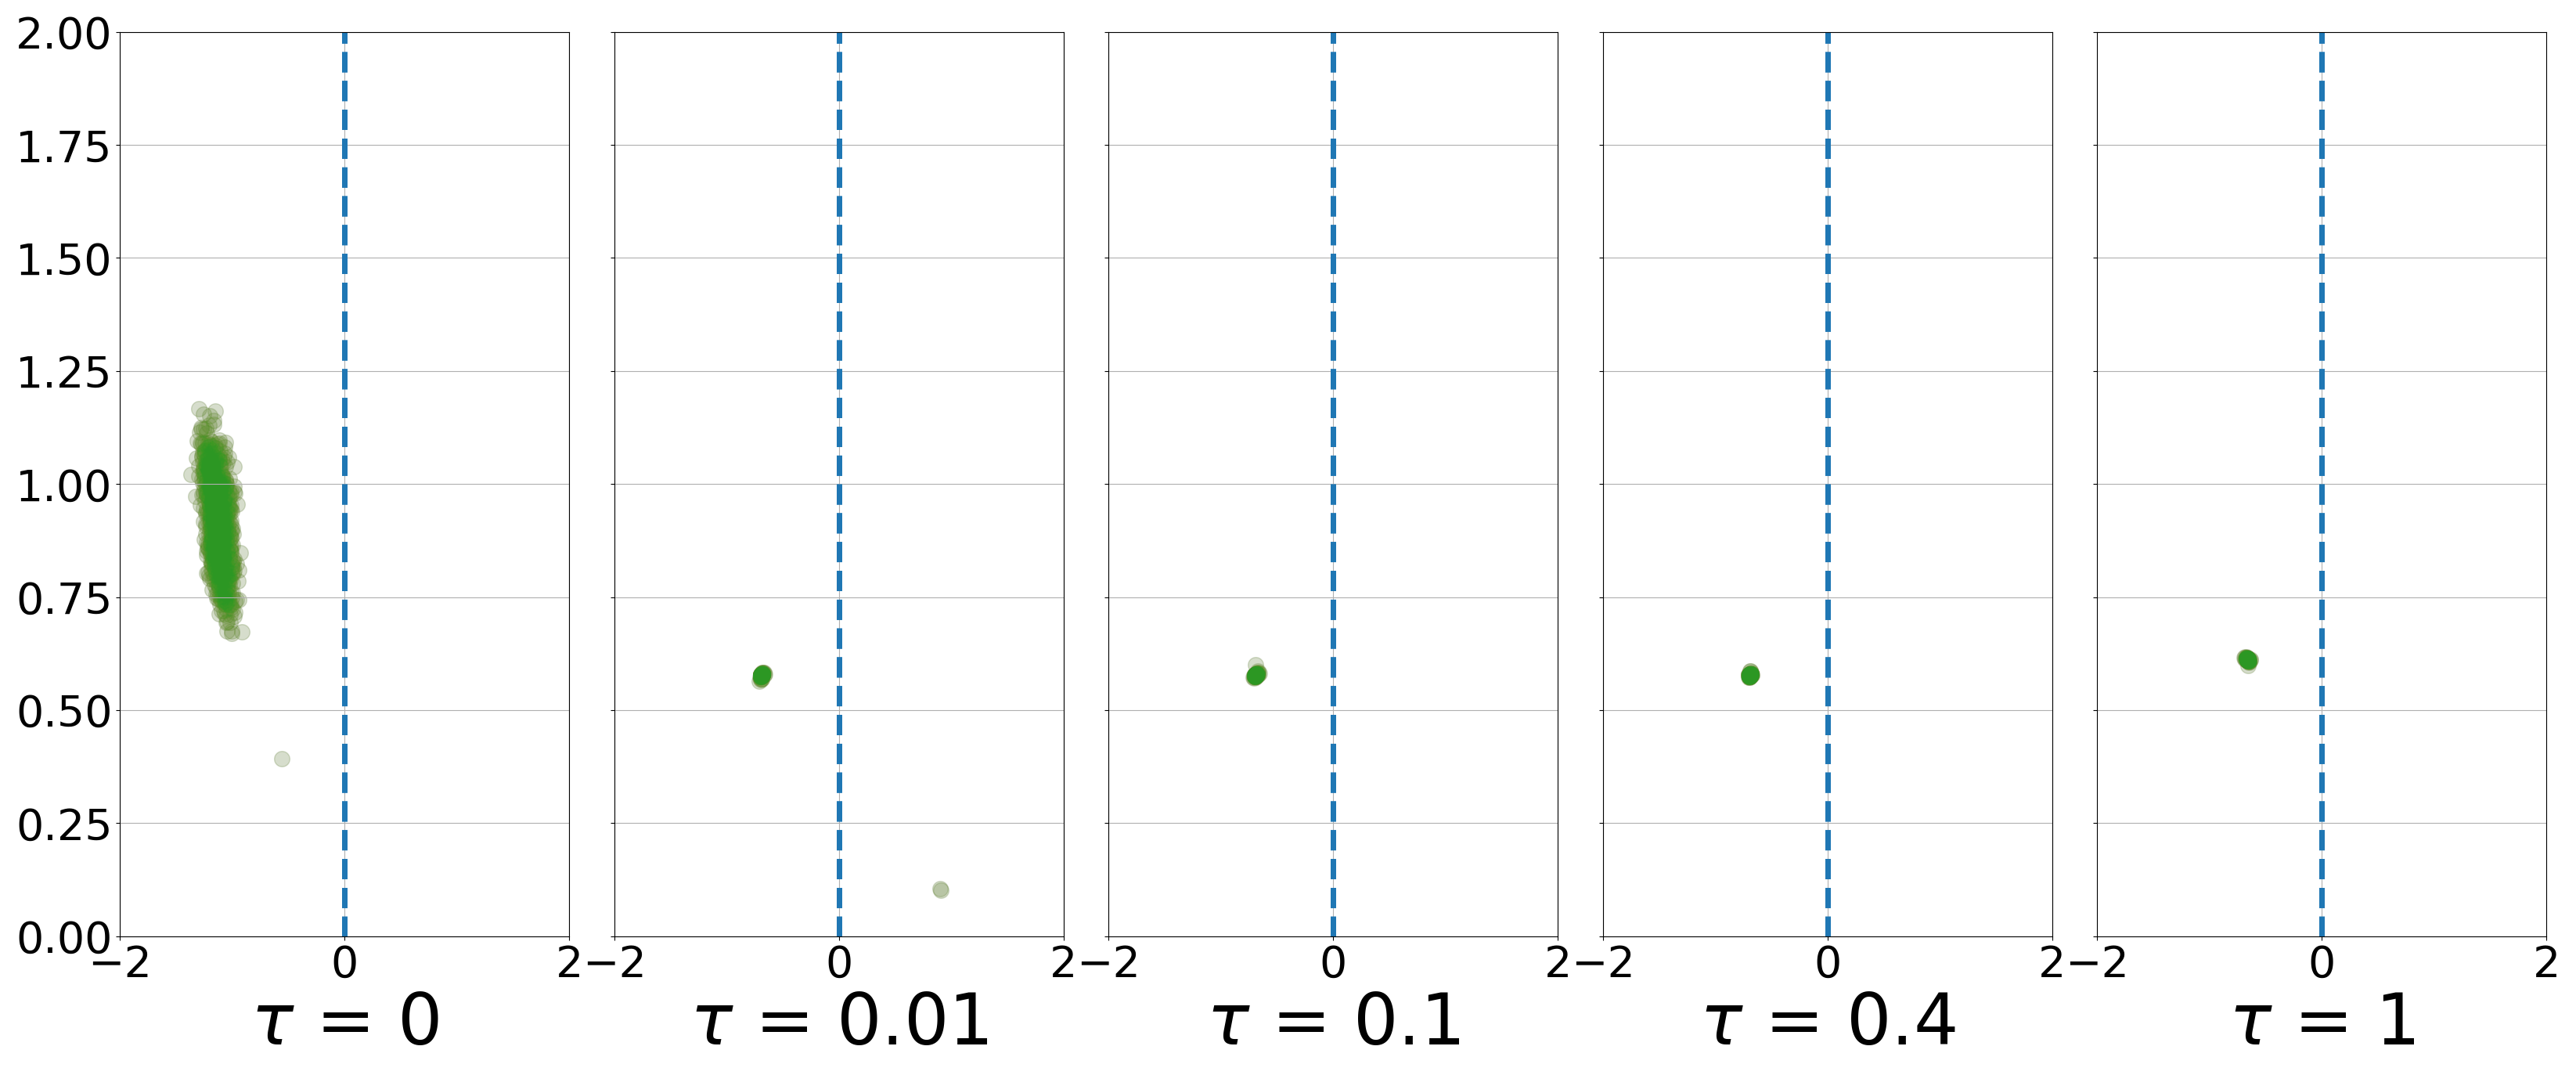
\includegraphics[width=\columnwidth]{figs/continuous-switch-stay/notlearnQ/state1_pi_forward_optim=rmsprop_lr=0.01.png}
    \caption{Forward KL on state 1.}
    \label{fig:cont-switch-stay-forward-s1}
  \end{subfigure}\hspace{15pt}
  
  \begin{subfigure}[b]{0.85\linewidth}
        \centering
        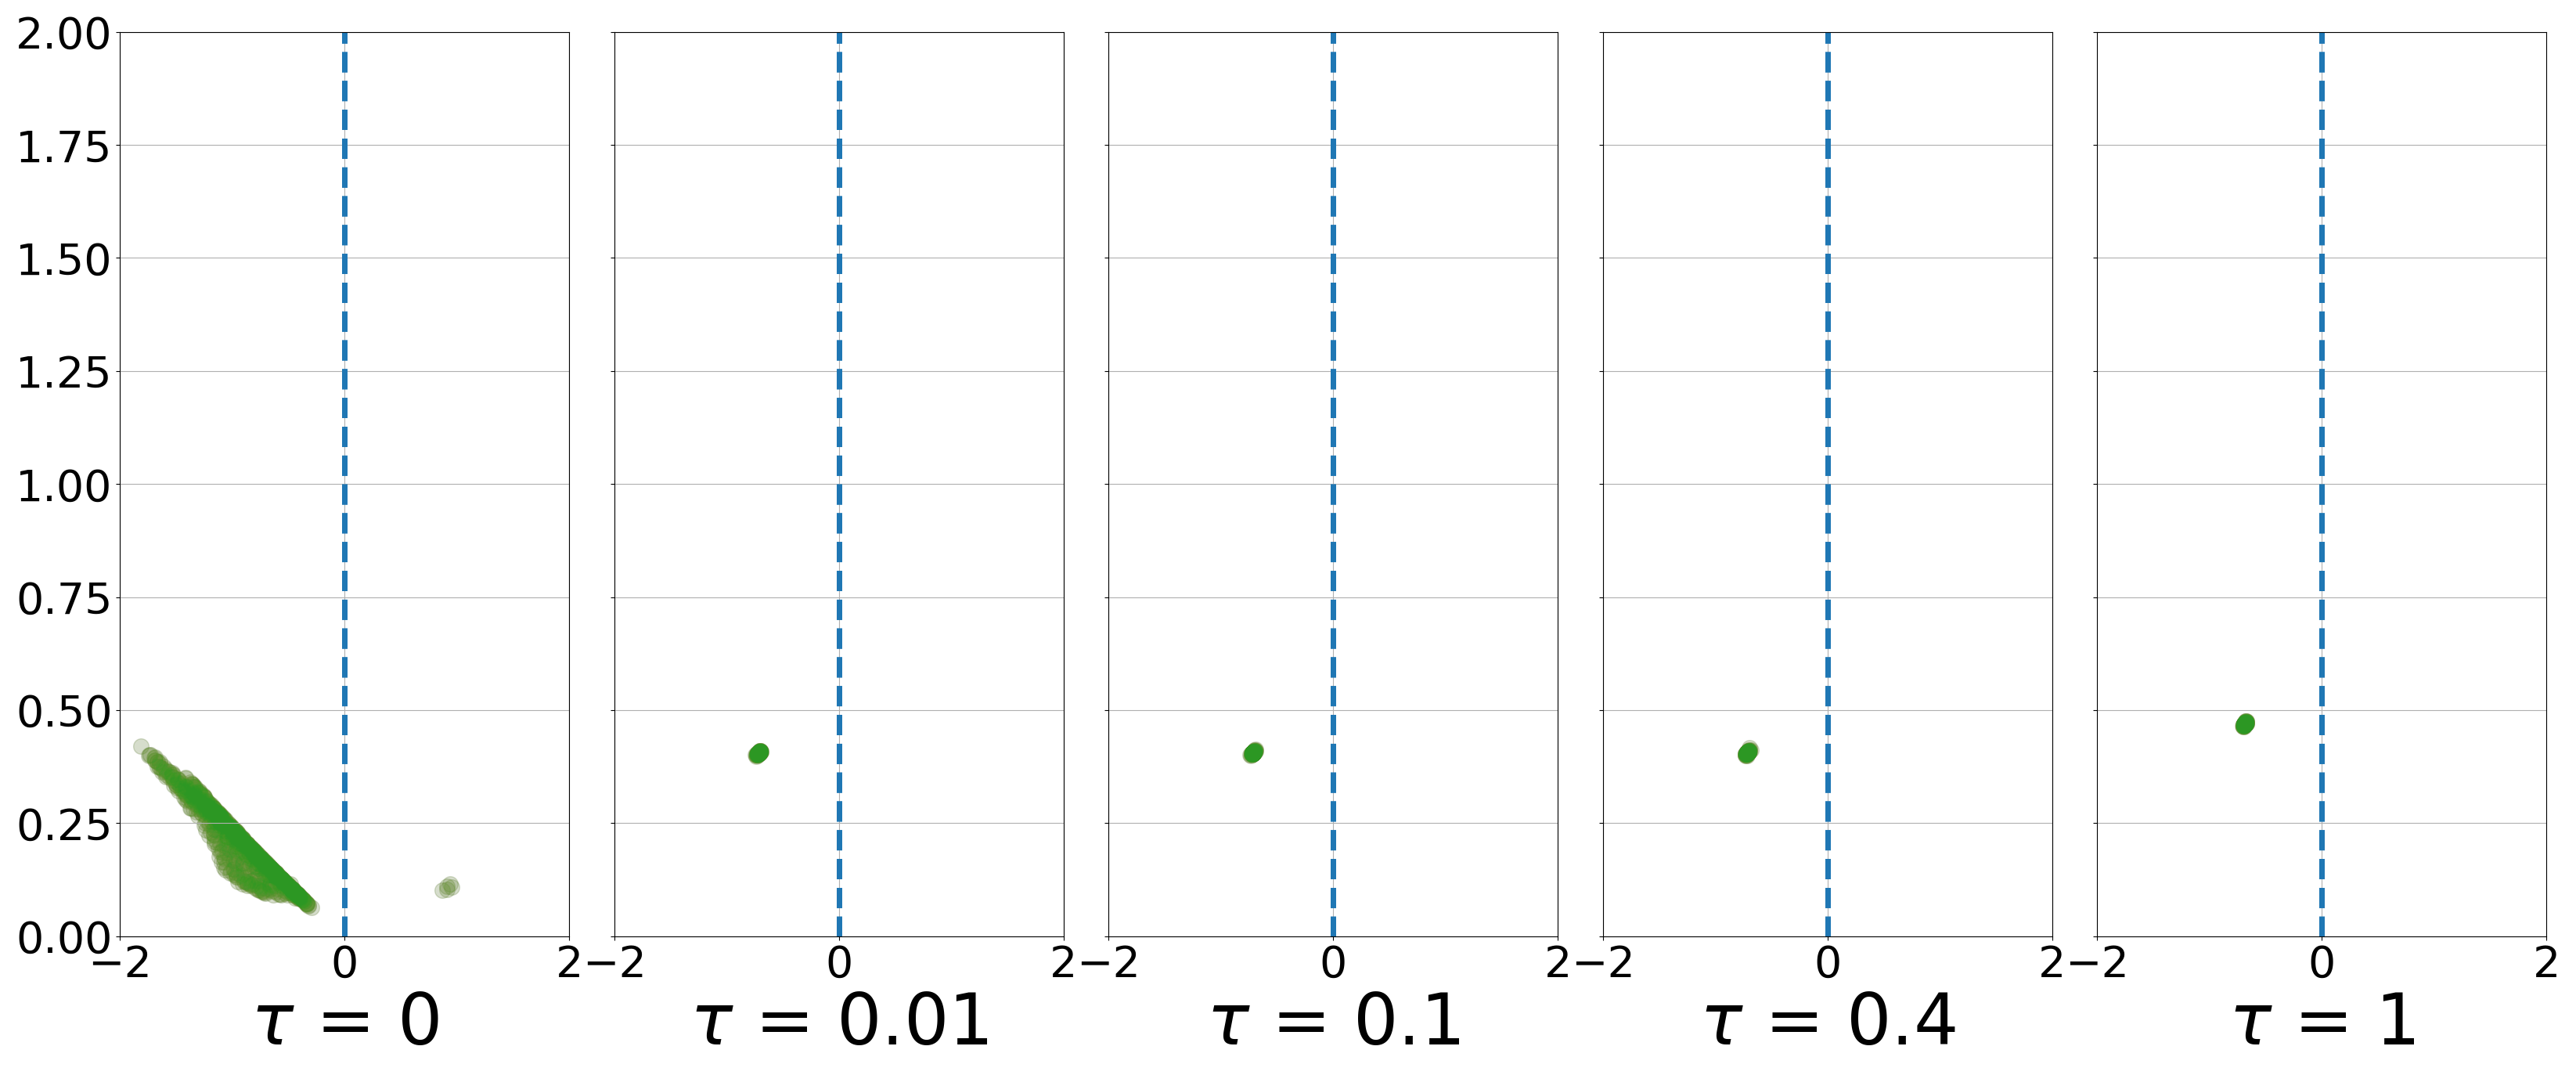
\includegraphics[width=\columnwidth]{figs/continuous-switch-stay/notlearnQ/state1_pi_reverse_optim=rmsprop_lr=0.01.png}
        \caption{Reverse KL on state 1.}
        \label{fig:cont-switch-stay-reverse-s1}
  \end{subfigure}
  \caption{See \Cref{fig:final-ss-probs-0}.}
  \label{fig:final-ss-probs-1}
\end{figure}

We also note here that when fewer integration points were used in an earlier version of this experiment, RKL exhibited substantial instability and a large number of iterates across temperatures and $\sigma_0$ values converged to suboptimal deterministic policies. This phenomenon might be related to the effect of stochasticity when approximating the KL loss, which is discussed in \Cref{sec:stochastic-microworld}.

 
\section{Discrete-Action Results}\label{sec:microworld-discrete-actions}

Overall, there is markedly less distinction between RKL and FKL in the discrete action setting with a softmax policy parameterization. In the heatmap in \Cref{fig:discrete-heatmap}, the loss surfaces for both KLs are very similar for a given temperature, in contrast to the heatmap for the continuous bandit. As the temperature increases, the black region (region with low loss) moves closer to the middle of the plot, which is consistent with the fact that the target distribution becomes closer to uniform as the temperature increases. 
\begin{figure}[!htb]
    \centering
    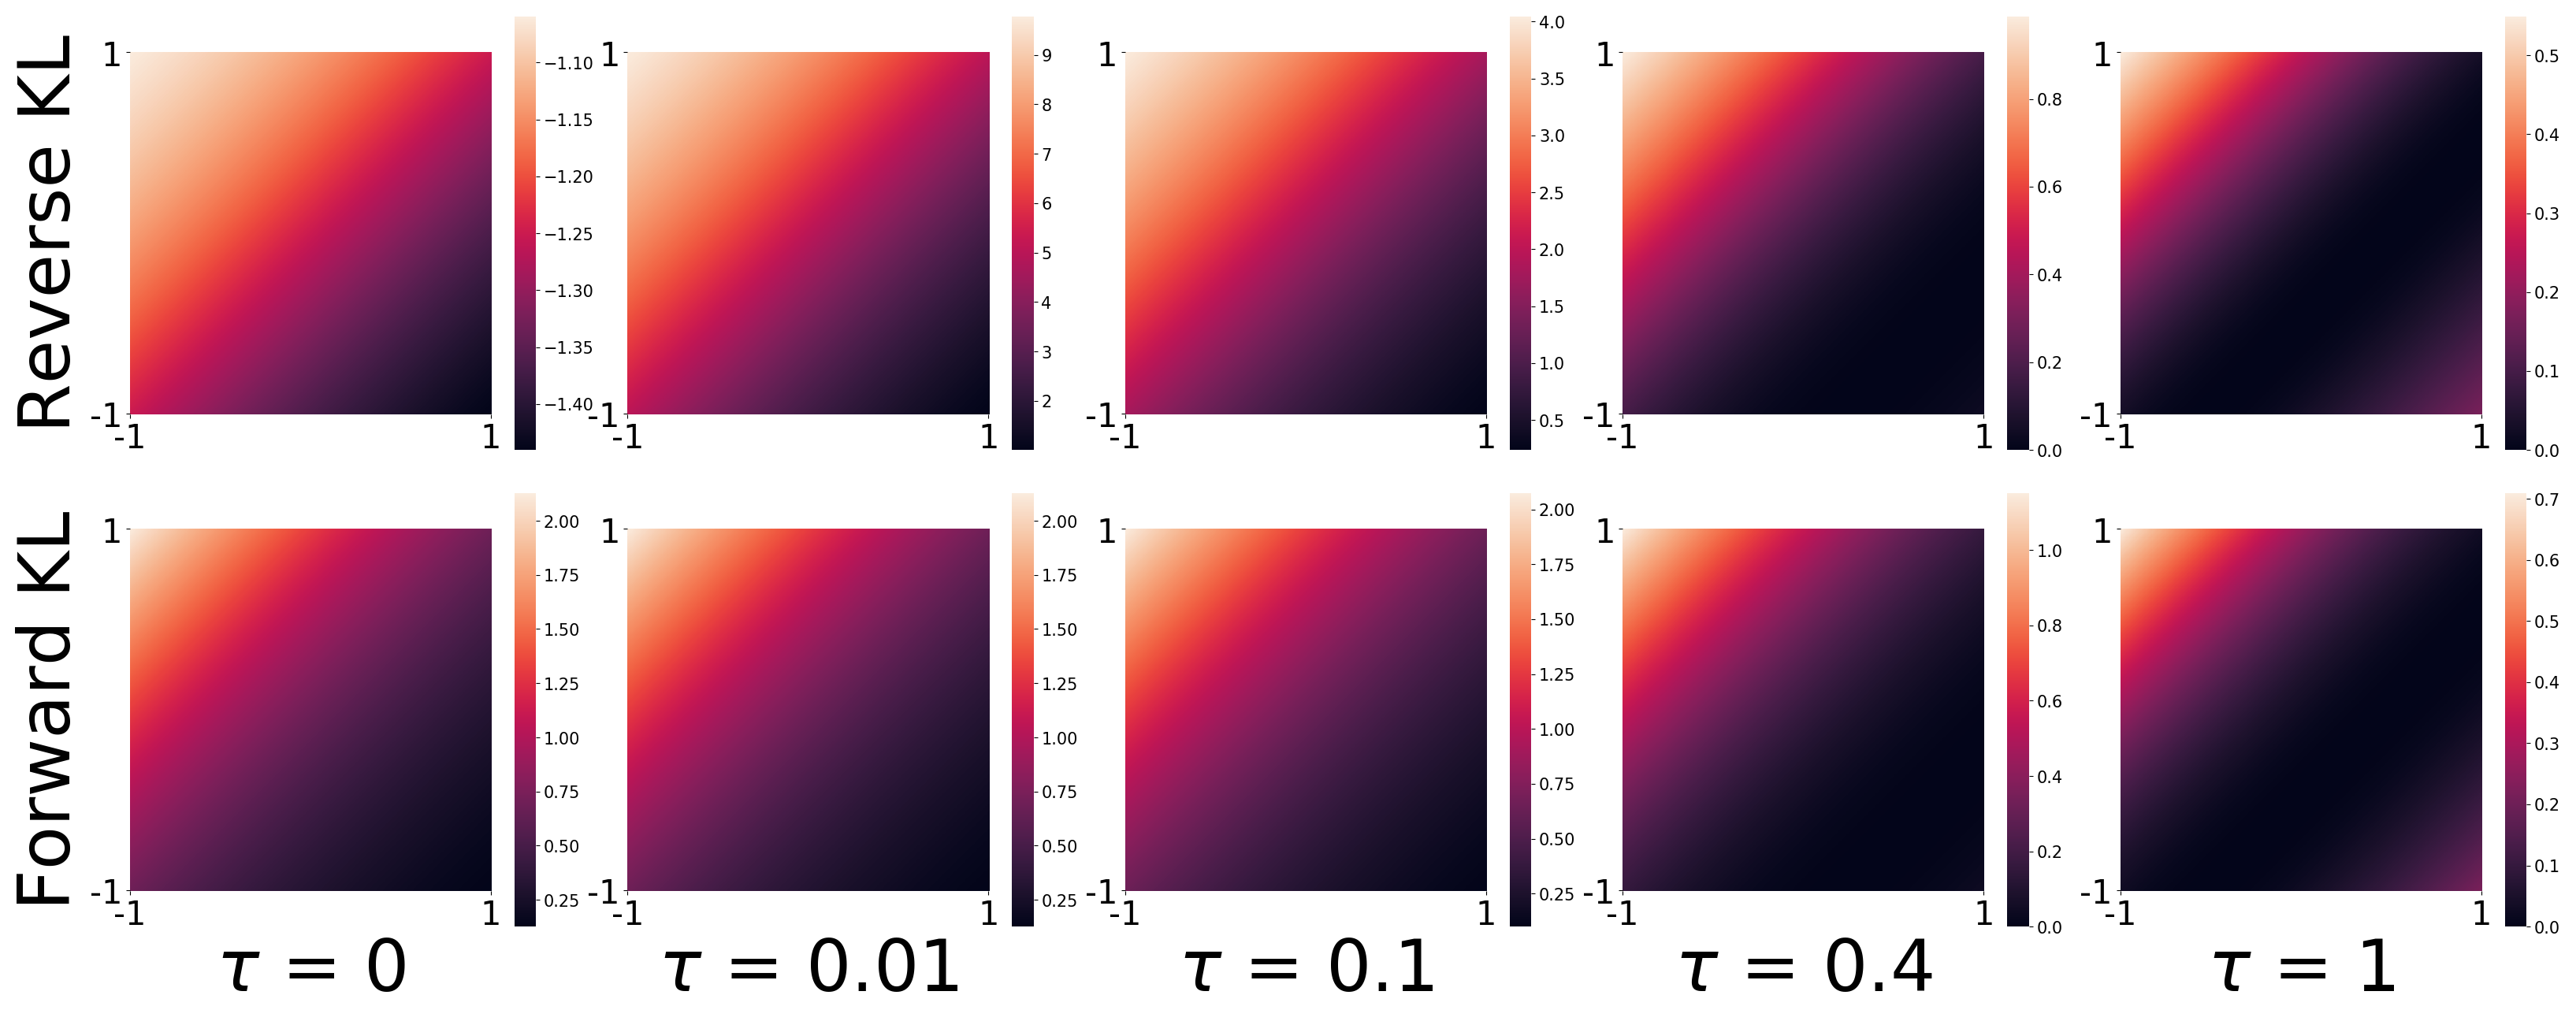
\includegraphics[width=1\columnwidth]{figs/discrete-bandit/heatmaps/discrete.png}
    \caption{Heatmap for the KLs on the discrete bandit. In a given subplot, the $x$-axis is the logit for the optimal arm and the $y$-axis is the logit for the suboptimal arm.}
    \label{fig:discrete-heatmap}
  \end{figure}

Next, we track the progress of 1000 iterates over 1000 gradient steps. For each iterate, we initialize each logit--one for each arm--uniformly in $(-1, 1)$. The behaviour policy is thus the result of the softmax function applied to the logit vector. 

When looking at 1000 iterates over 1000 gradient steps, both RKL and FKL iterates learn the optimal arms in \Cref{fig:discrete-bandit-prob-forward-rmsprop,fig:discrete-bandit-prob-reverse-rmsprop}. There is little difference in the behaviour of iterates under either KL; there seems just to be one global optimum to which iterates under either KL converge reliably. 

% \begin{figure}[!htb]
%   \centering
%   \begin{subfigure}[b]{1\linewidth}
%     \centering
%     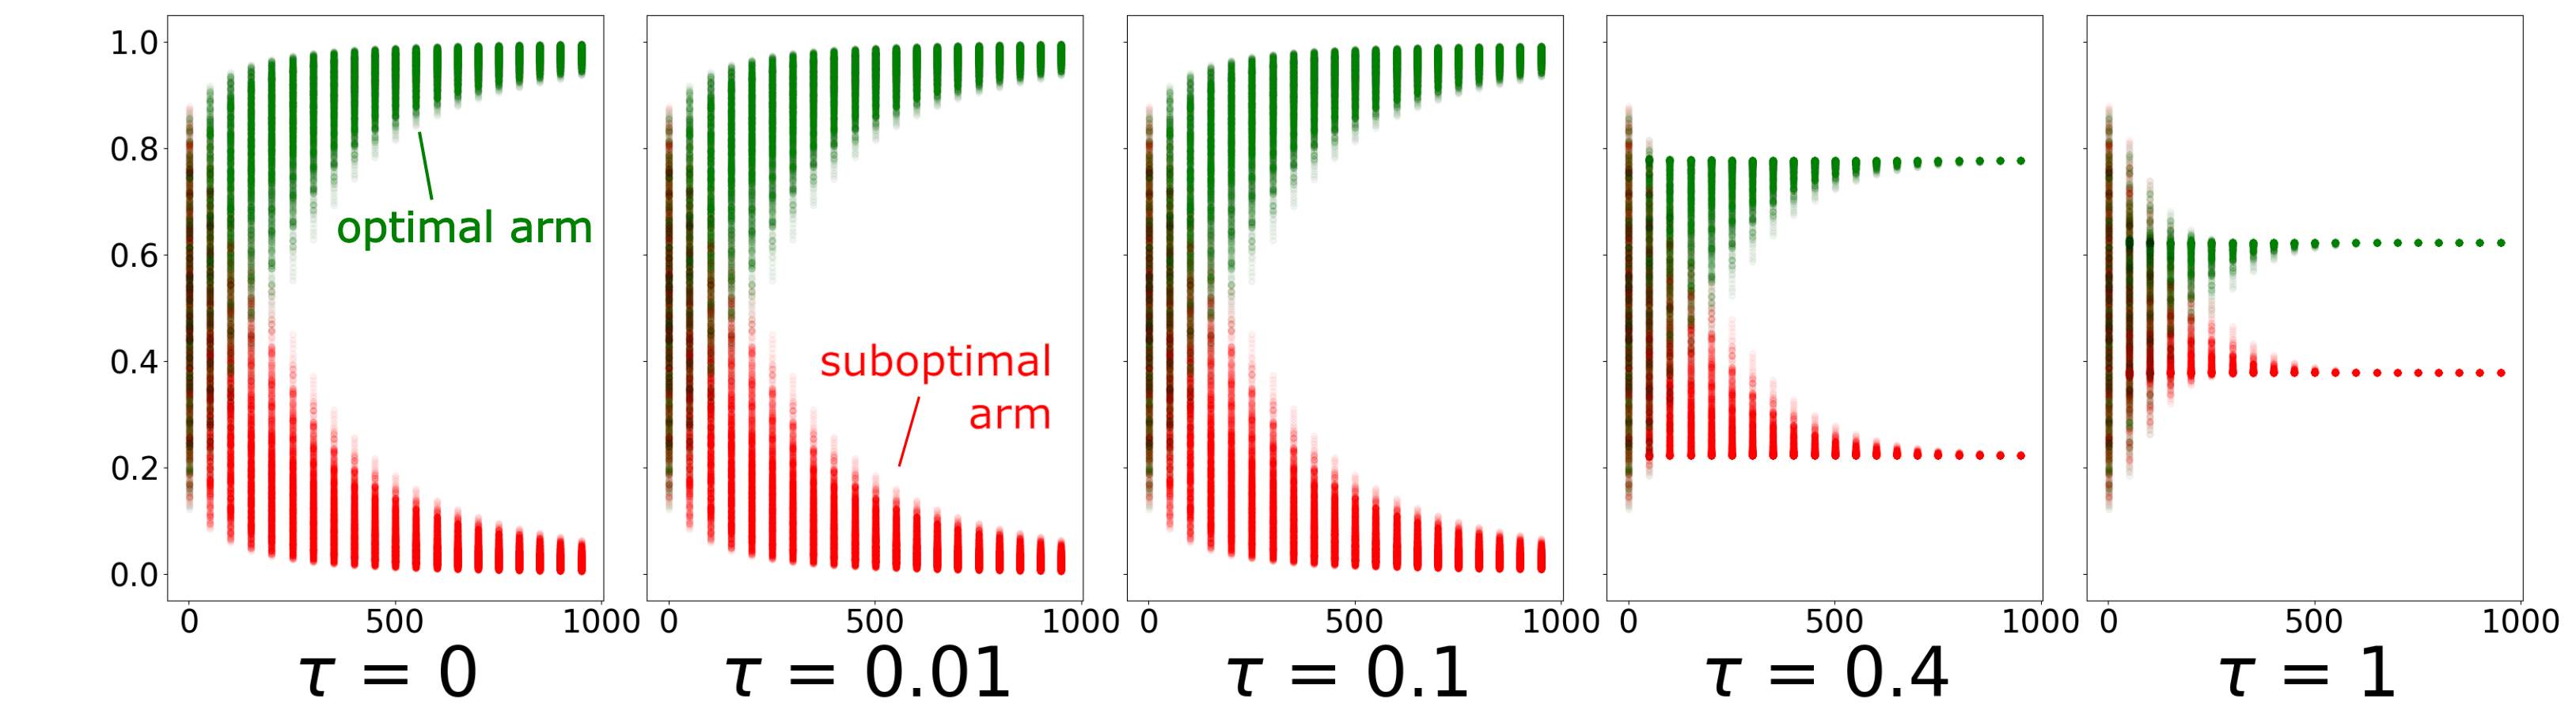
\includegraphics[width=1\columnwidth]{figs/discrete-bandit/notlearnQ/adam/prob-adam.png}
%     \caption{Forward KL, Adam.}
%     \label{fig:discrete-bandit-prob-forward-adam}
%   \end{subfigure}%
  
%   \begin{subfigure}[b]{1\linewidth}
%     \centering
%     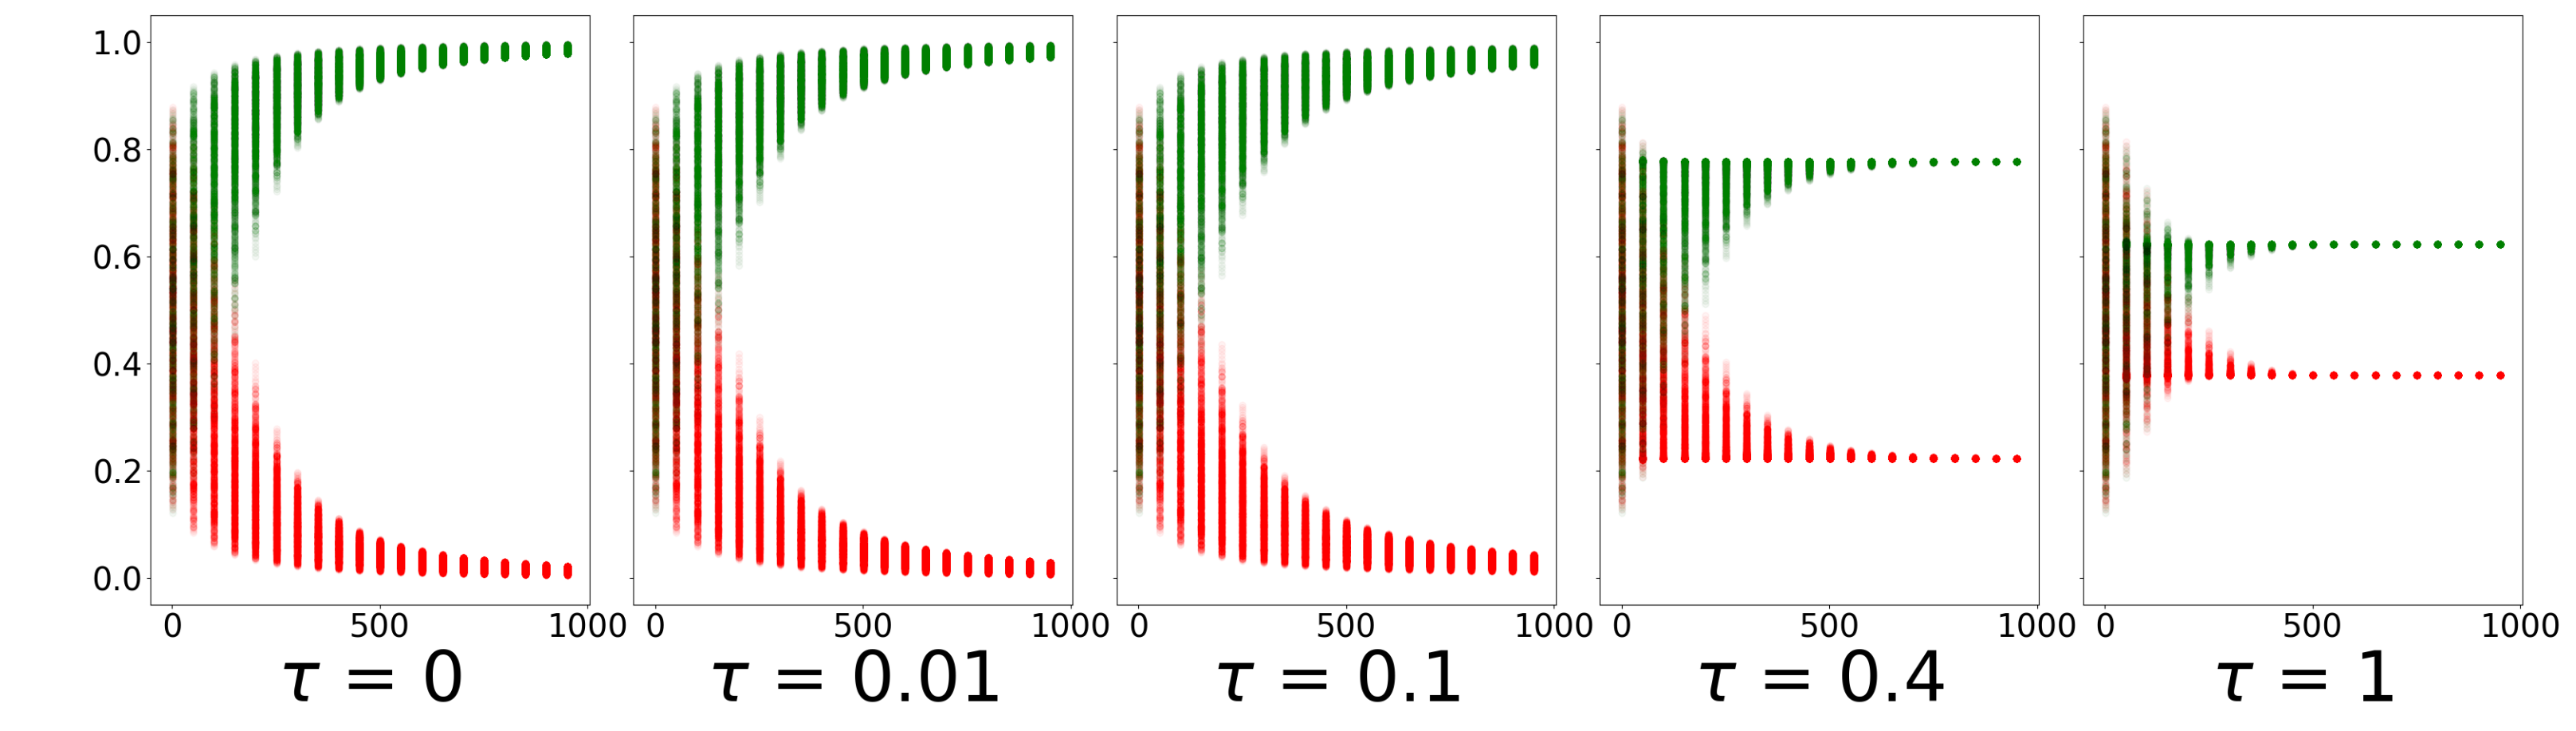
\includegraphics[width=1\columnwidth]{figs/discrete-bandit/notlearnQ/adam/prob-reverse-adam.png}
%     \caption{Reverse KL, Adam. }
%     \label{fig:discrete-bandit-prob-reverse-adam}
%   \end{subfigure}
%   \caption{Each subplot tracks the learned probability of each arm for 1000 iterates over 1000 gradient steps. The learning rate is set to be 0.005 and Adam is the optimizer. }
% \end{figure}

\begin{figure}[!htb]
  \centering
  \begin{subfigure}[b]{1\linewidth}
    \centering
    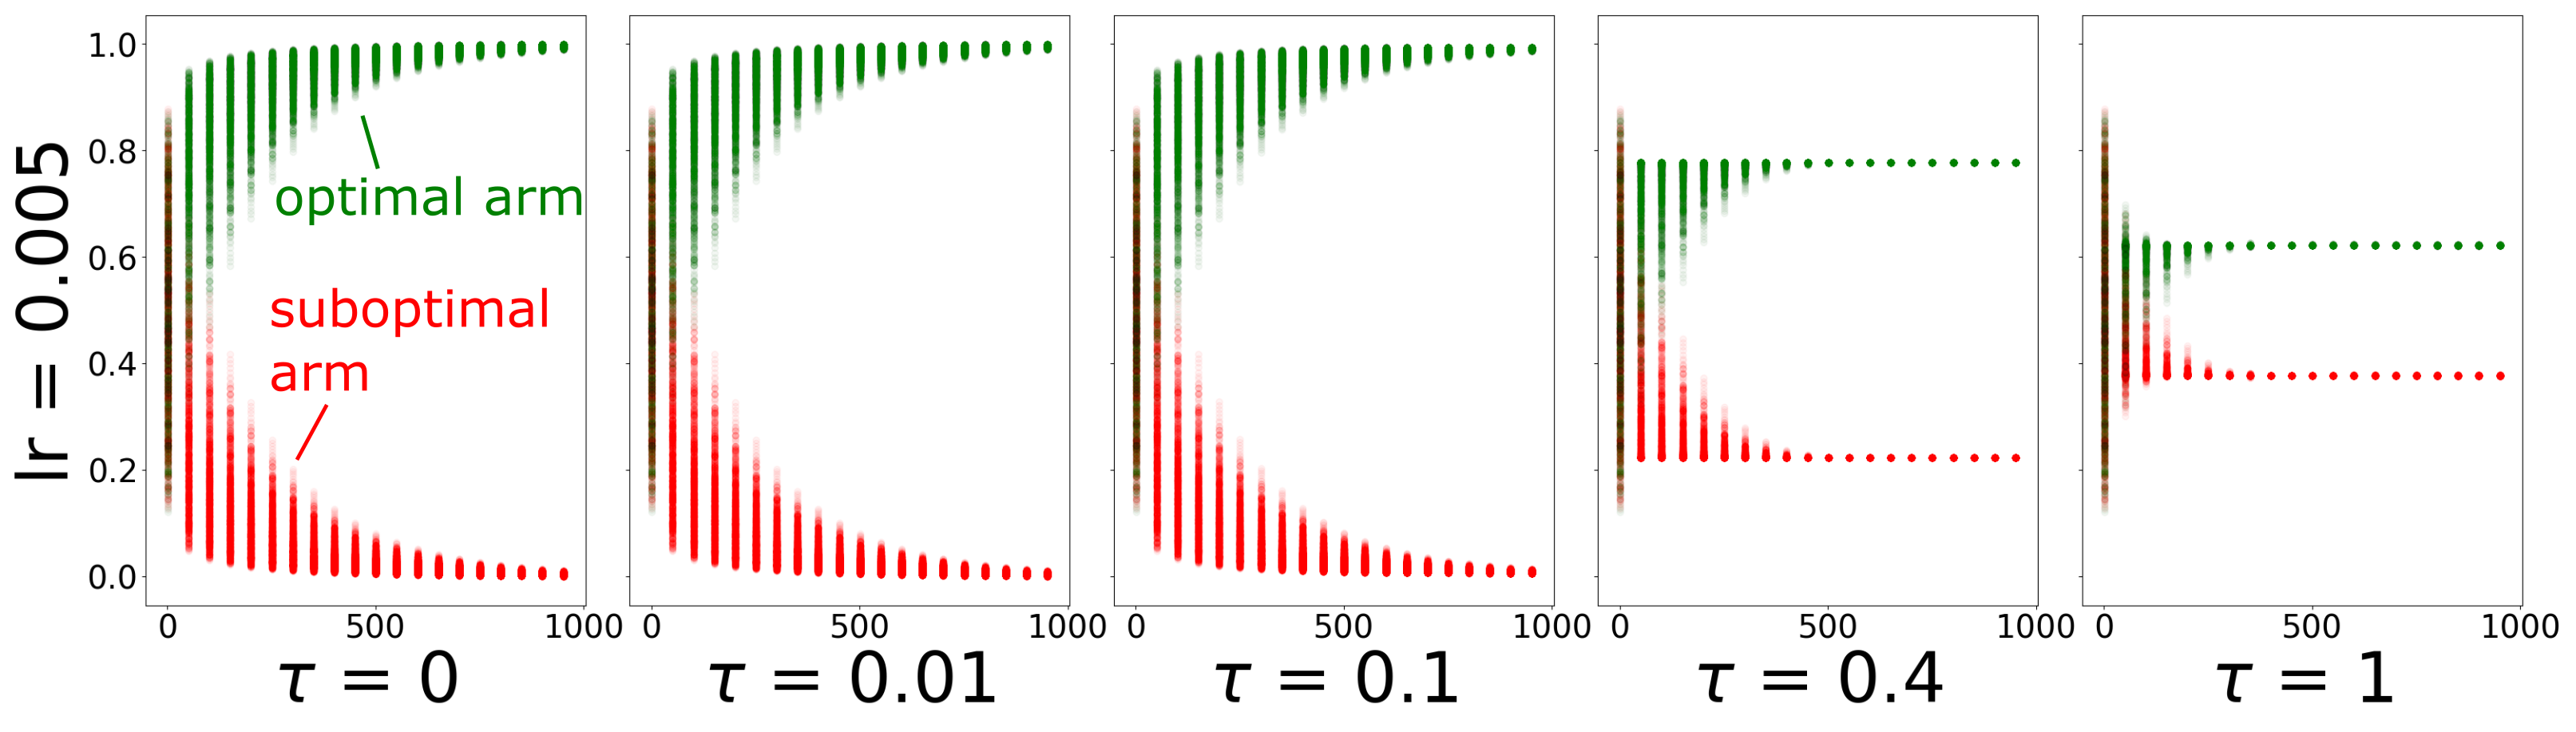
\includegraphics[width=1\columnwidth]{figs/discrete-bandit/notlearnQ/rmsprop/prob_forward_optim=rmsprop_lr=0.005.png}
    \caption{Forward KL.}
    \label{fig:discrete-bandit-prob-forward-rmsprop}
  \end{subfigure}%
  
  \begin{subfigure}[b]{1\linewidth}
    \centering
    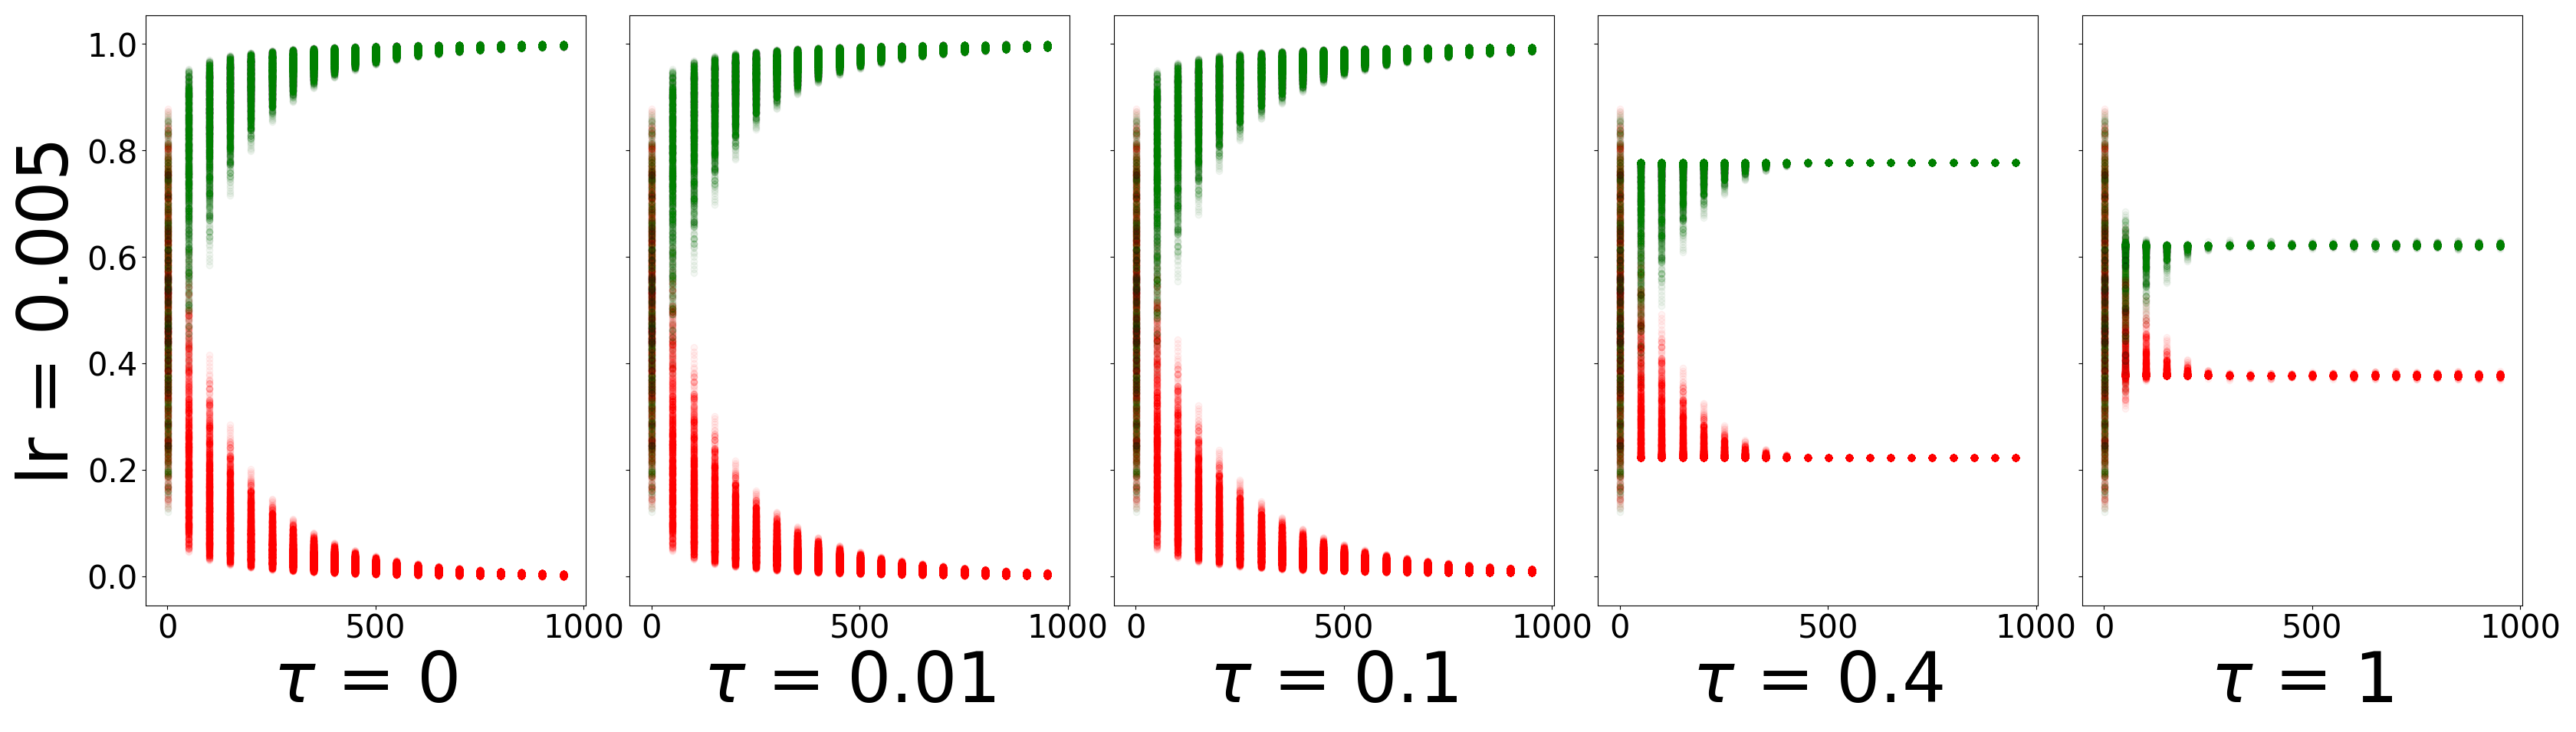
\includegraphics[width=1\columnwidth]{figs/discrete-bandit/notlearnQ/rmsprop/prob_reverse_optim=rmsprop_lr=0.005.png}
    \caption{Reverse KL. }
    \label{fig:discrete-bandit-prob-reverse-rmsprop}
  \end{subfigure}
  \caption{Each subplot tracks the learned probability of each arm for 1000 iterates over 1000 gradient steps. The learning rate is set to be 0.005. }
\end{figure}


Results for discrete Switch-Stay are in \Cref{fig:discrete-ss-all}. Both FKL and RKL iterates move in the direction of the optimal value function, but RKL iterates seem to converge faster. While a difference in convergence speed did also exist on the continuous version of Switch-Stay, the distinction is less notable here. 

For higher temperatures, the limit point of the iterates is slightly further away from the optimal value function of the original MDP than for lower temperatures. This result is to be expected given that in general, the optimal entropy-regularized policy is different from the optimal non-regularized policy \citep{geist2019theory}.

% \begin{figure}[!htb]
%   \centering
%   \begin{subfigure}[b]{0.5\linewidth}
%     \centering
%     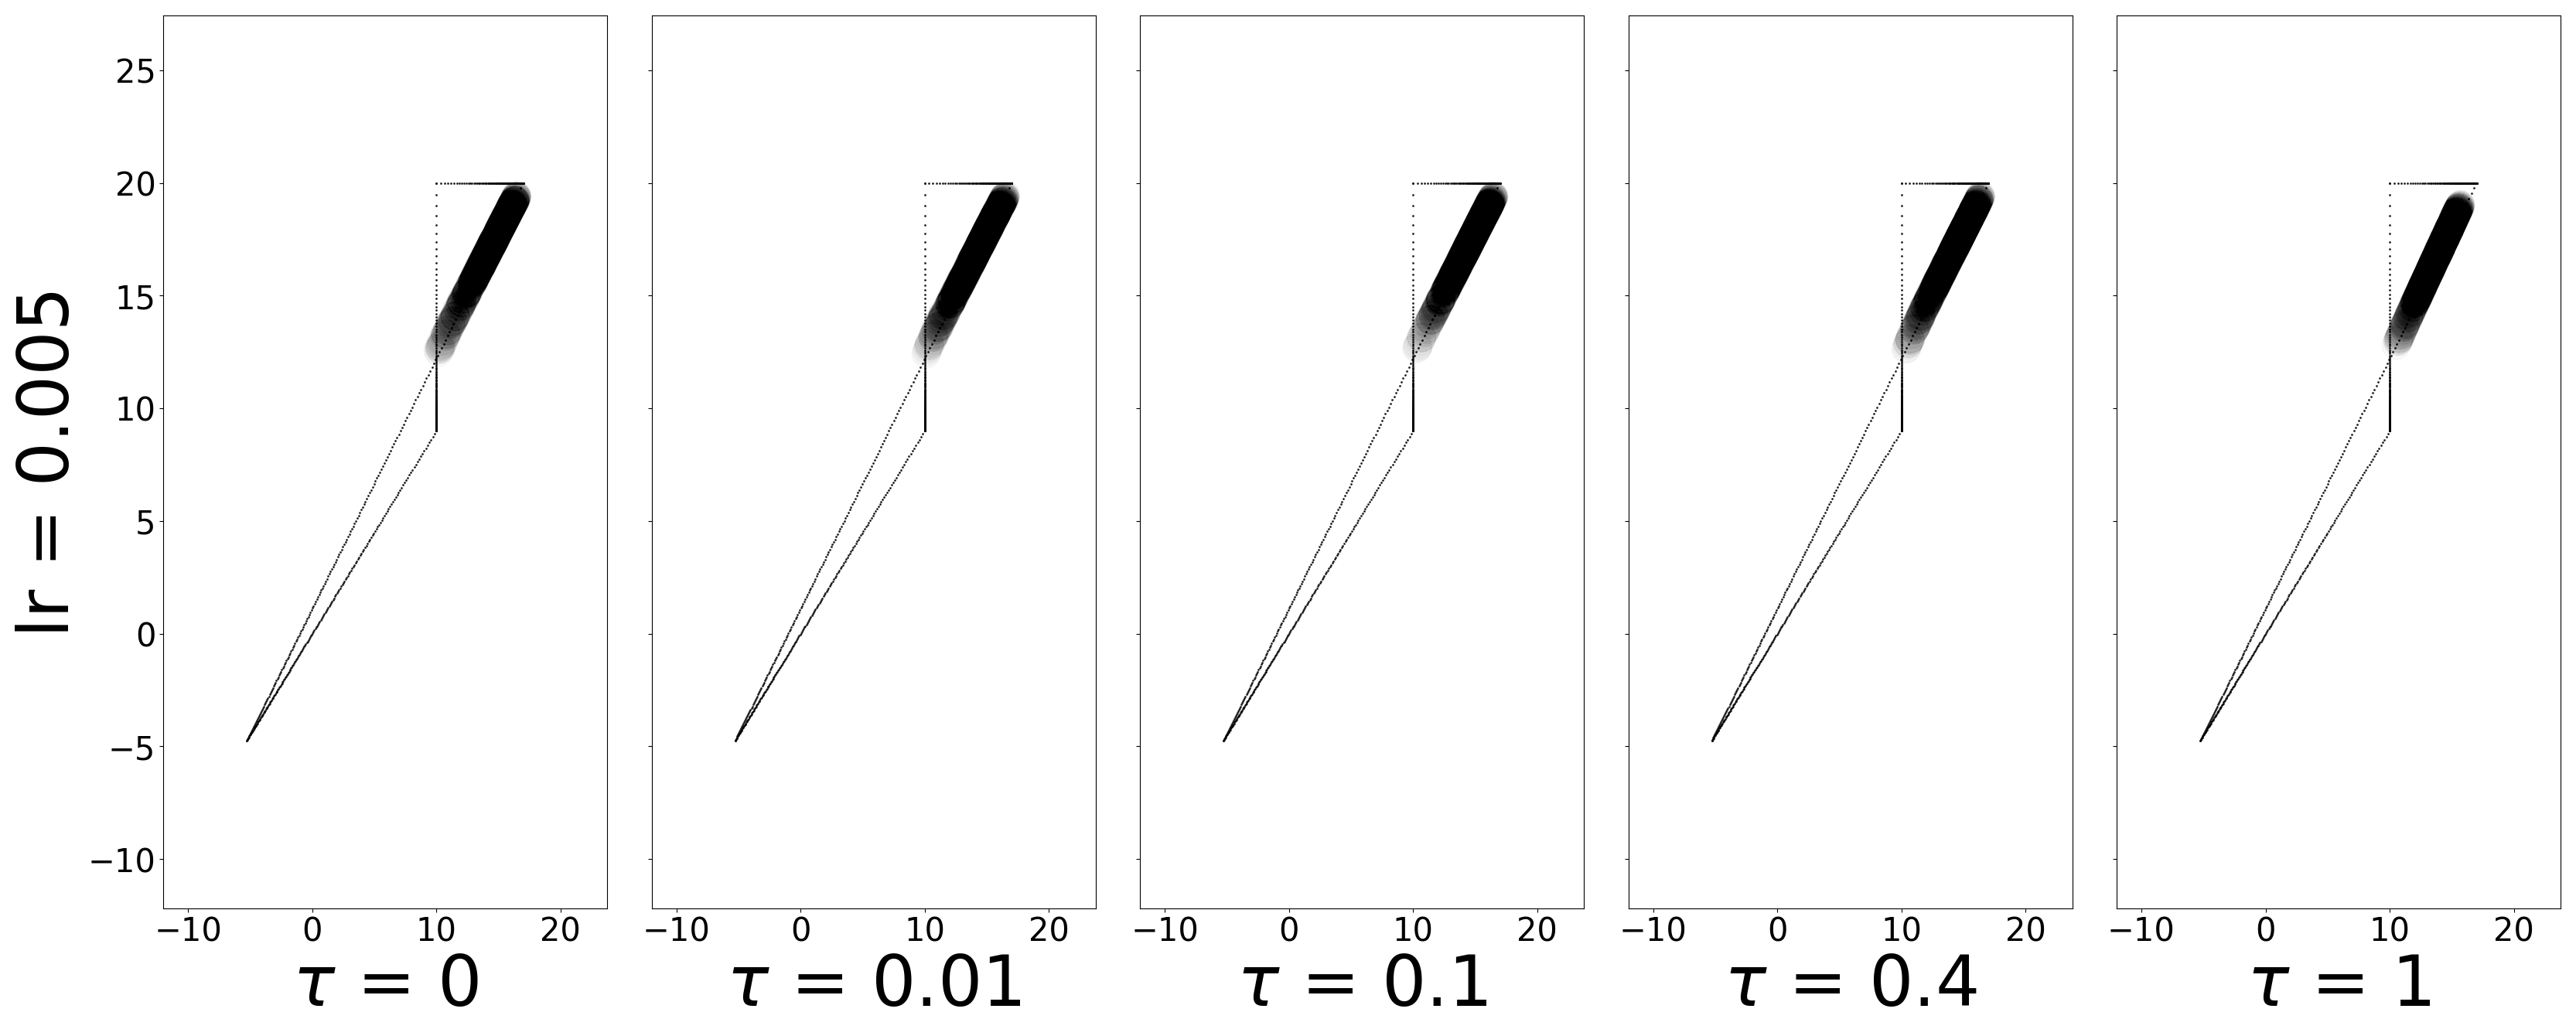
\includegraphics[width=0.8\columnwidth]{figs/switch-stay/notlearnQ/polytope_forward_optim=adam.png}
%     \caption{Forward KL.}
%     \label{fig:discrete-switch-stay-forward-adam}
%   \end{subfigure}%
%   \begin{subfigure}[b]{0.5\linewidth}
%         \centering
%         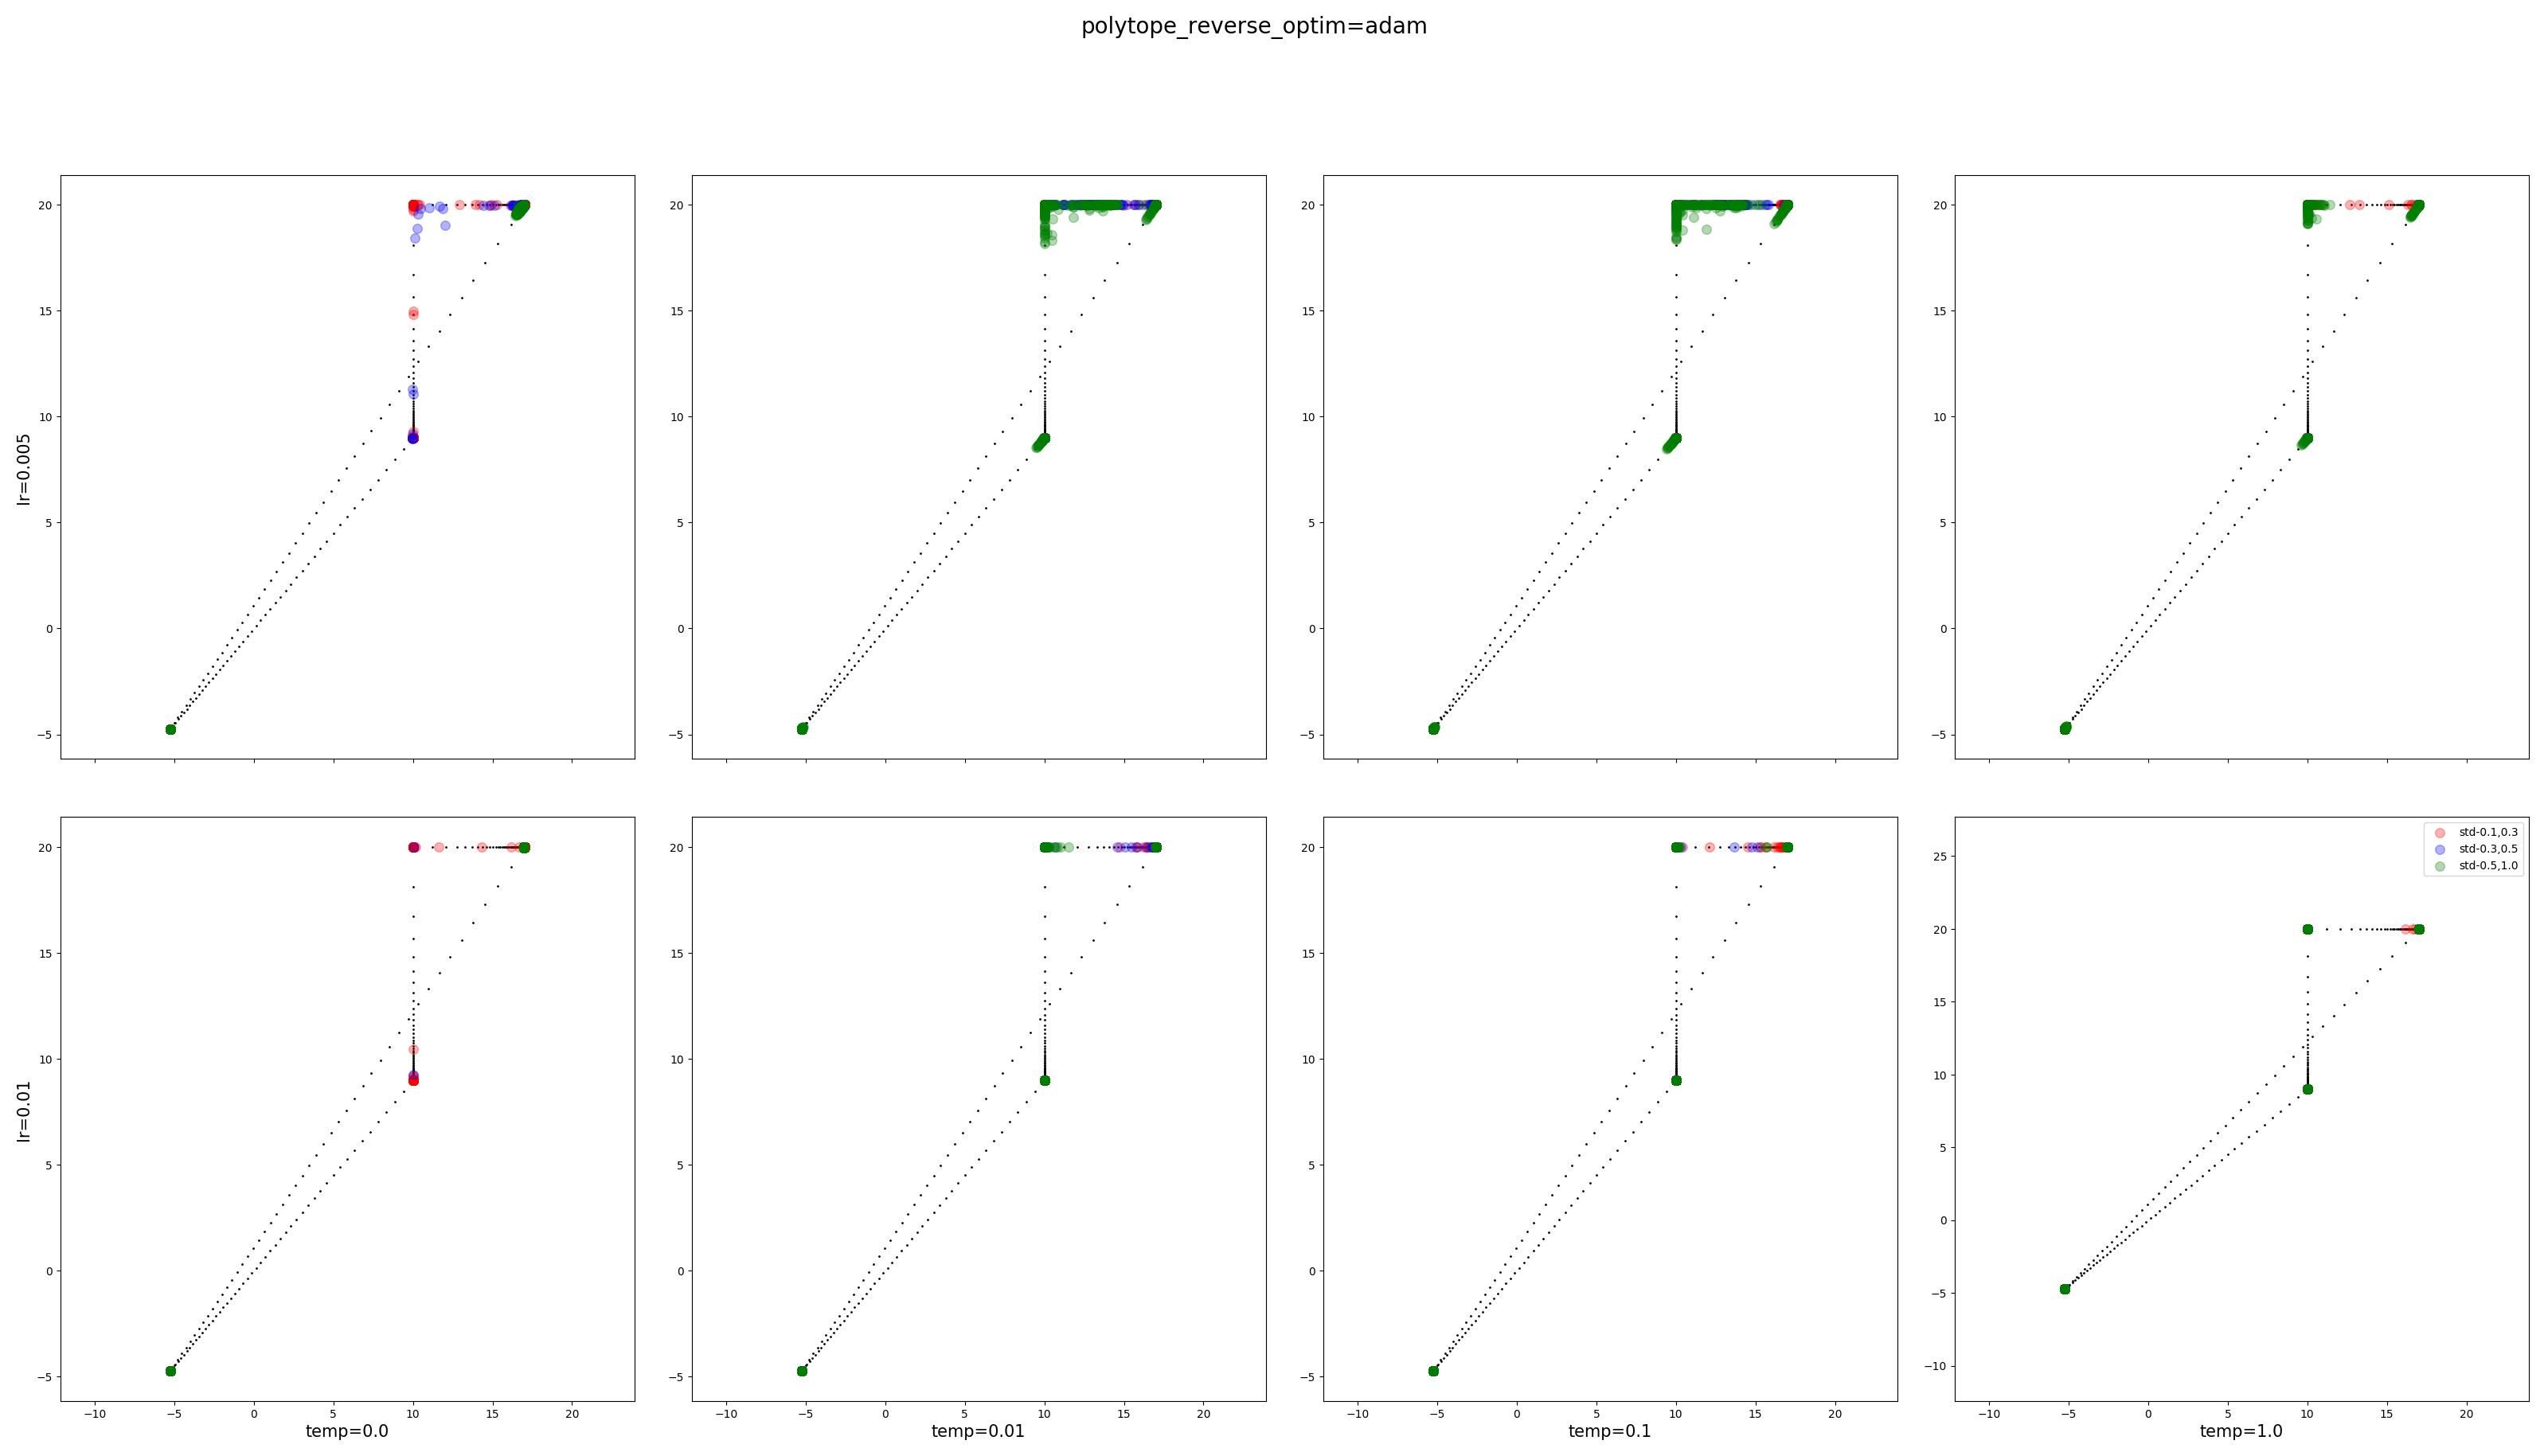
\includegraphics[width=0.8\columnwidth]{figs/switch-stay/notlearnQ/polytope_reverse_optim=adam.png}
%         \caption{Reverse KL.}
%         \label{fig:discrete-switch-stay-reverse-adam}
%   \end{subfigure}
%   \caption{Final value functions on discrete version of switch-stay after 500 gradient steps, $\gamma = 0.9$. Using Adam.}
% \end{figure}

% \begin{figure}[!htb]
%   \centering
%   \begin{subfigure}[b]{0.85\linewidth}
%     \centering
%     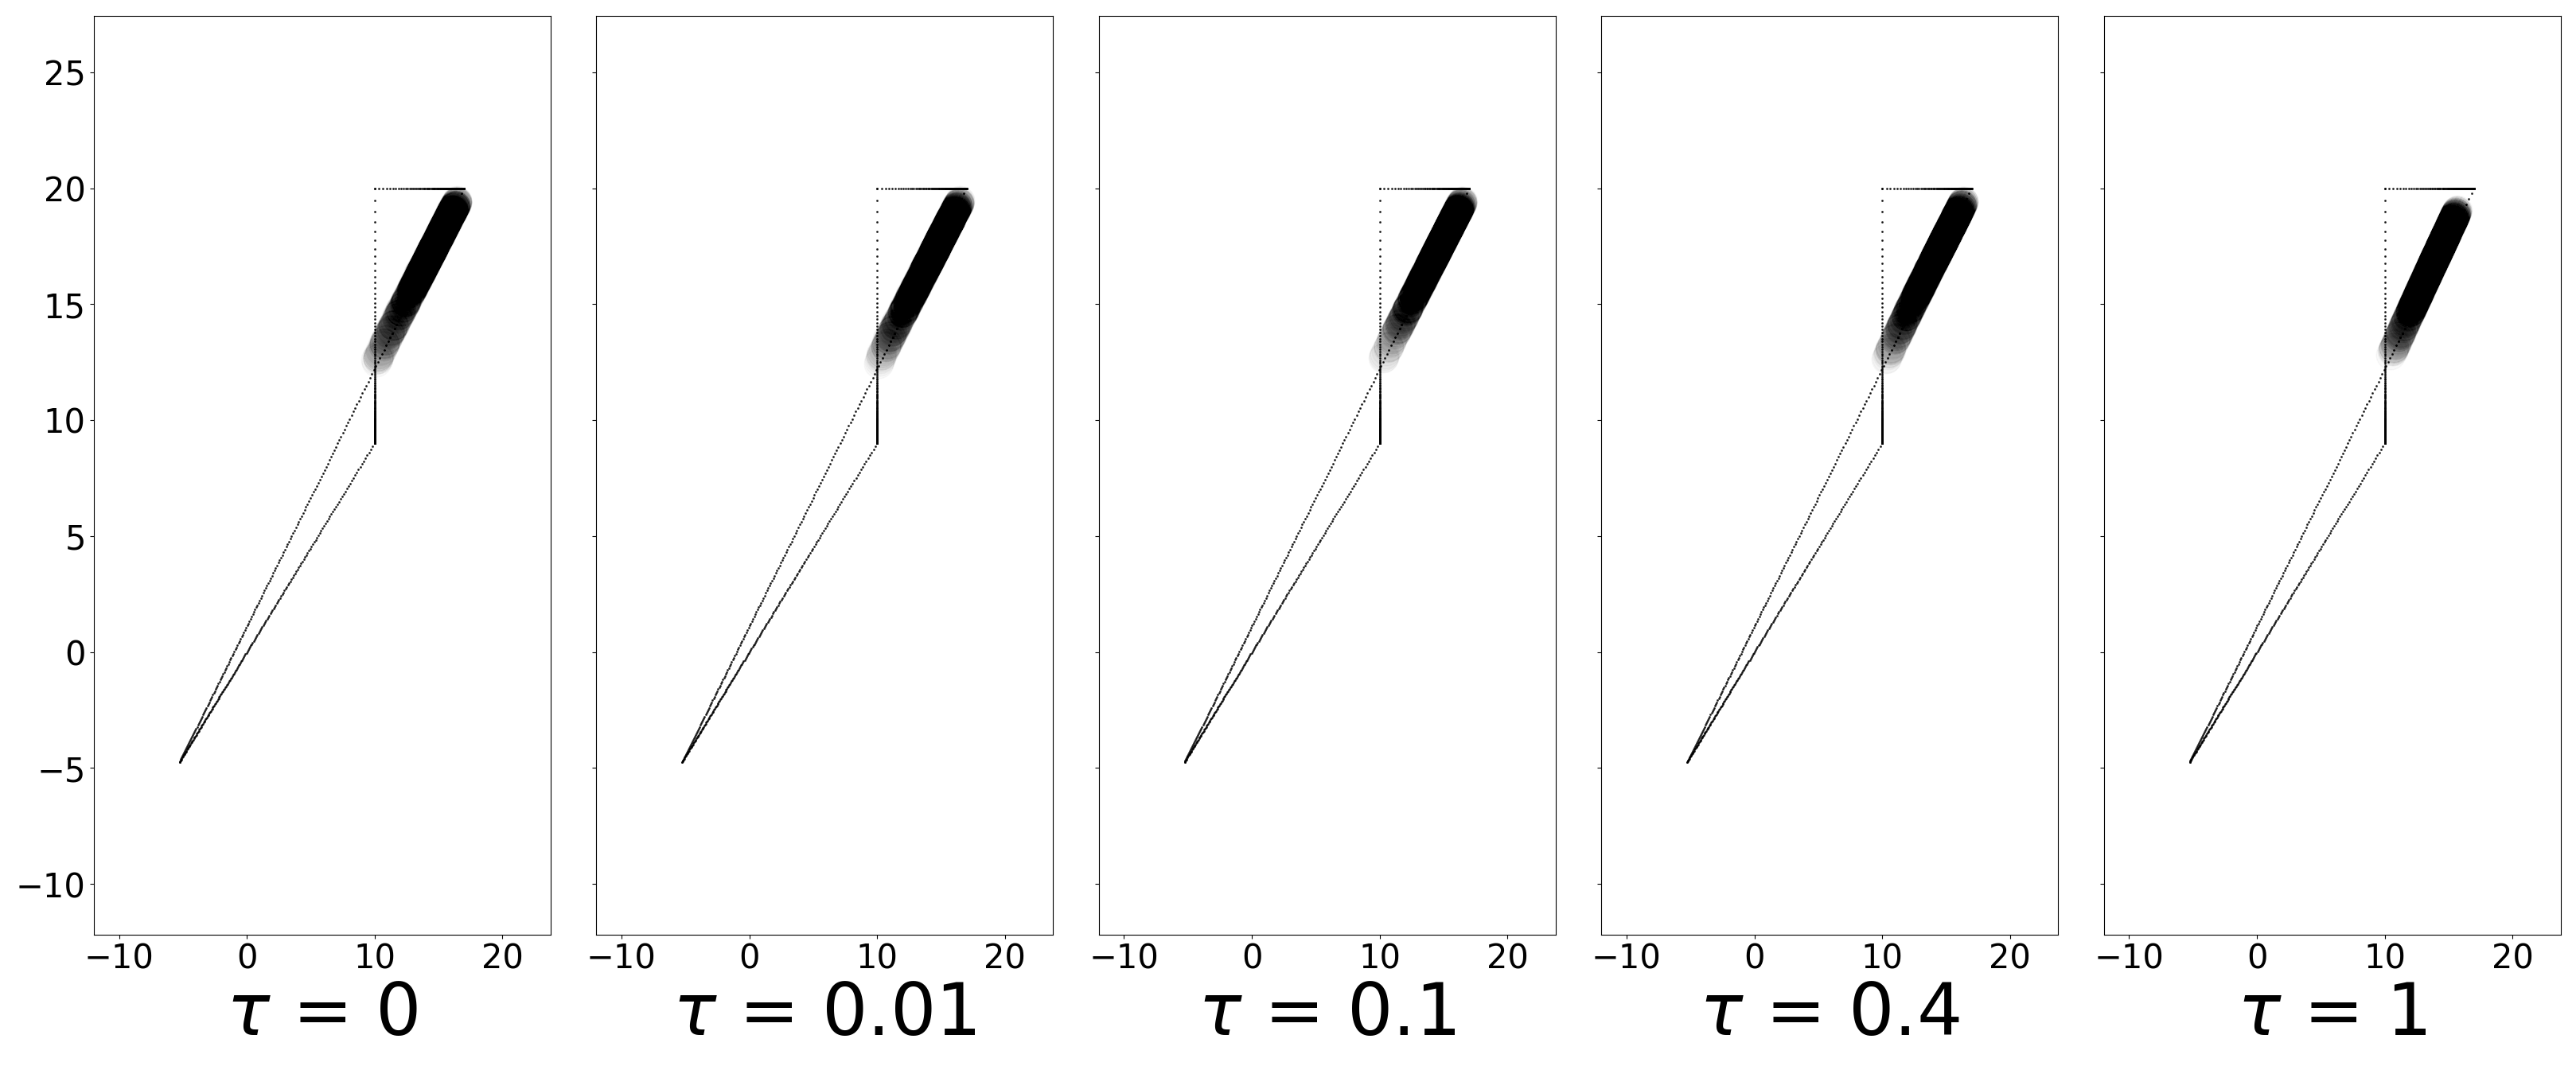
\includegraphics[width=0.8\columnwidth]{figs/switch-stay/notlearnQ/polytope_forward_optim=adam_lr=[0.005].png}
%     \caption{Forward KL, learning rate = 0.005.}
%     \label{fig:discrete-switch-stay-forward-adam0.005}
%   \end{subfigure}
  
%   \begin{subfigure}[b]{0.85\linewidth}
%         \centering
%         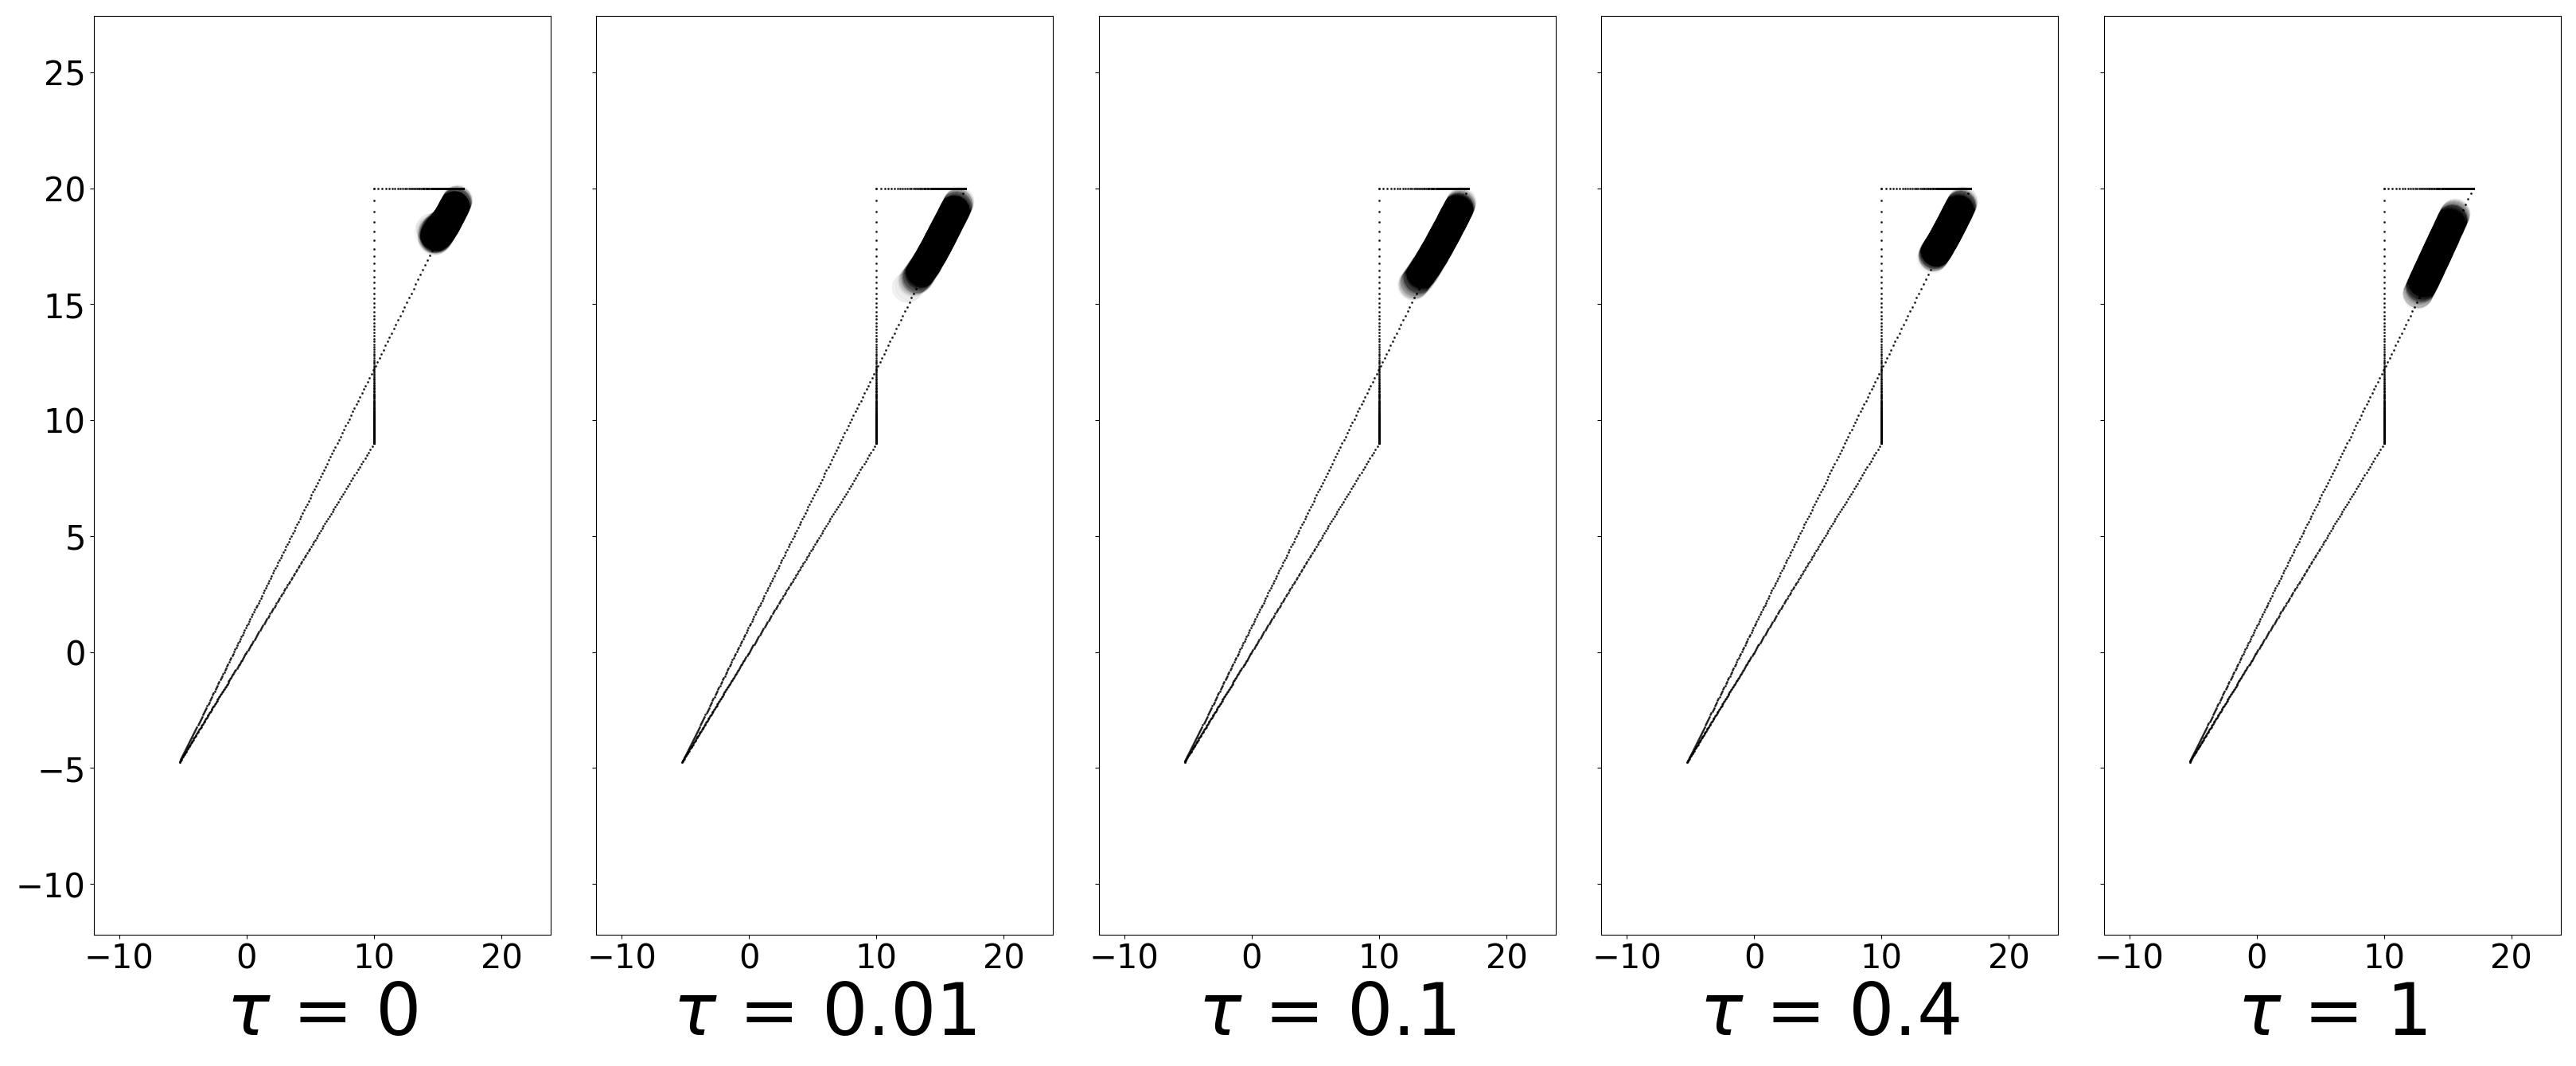
\includegraphics[width=0.8\columnwidth]{figs/switch-stay/notlearnQ/polytope_reverse_optim=adam_lr=[0.005].png}
%         \caption{Reverse KL, learning rate = 0.005.}
%         \label{fig:discrete-switch-stay-reverse-adam0.005}
%   \end{subfigure}
  
%   \begin{subfigure}[b]{0.85\linewidth}
%     \centering
%     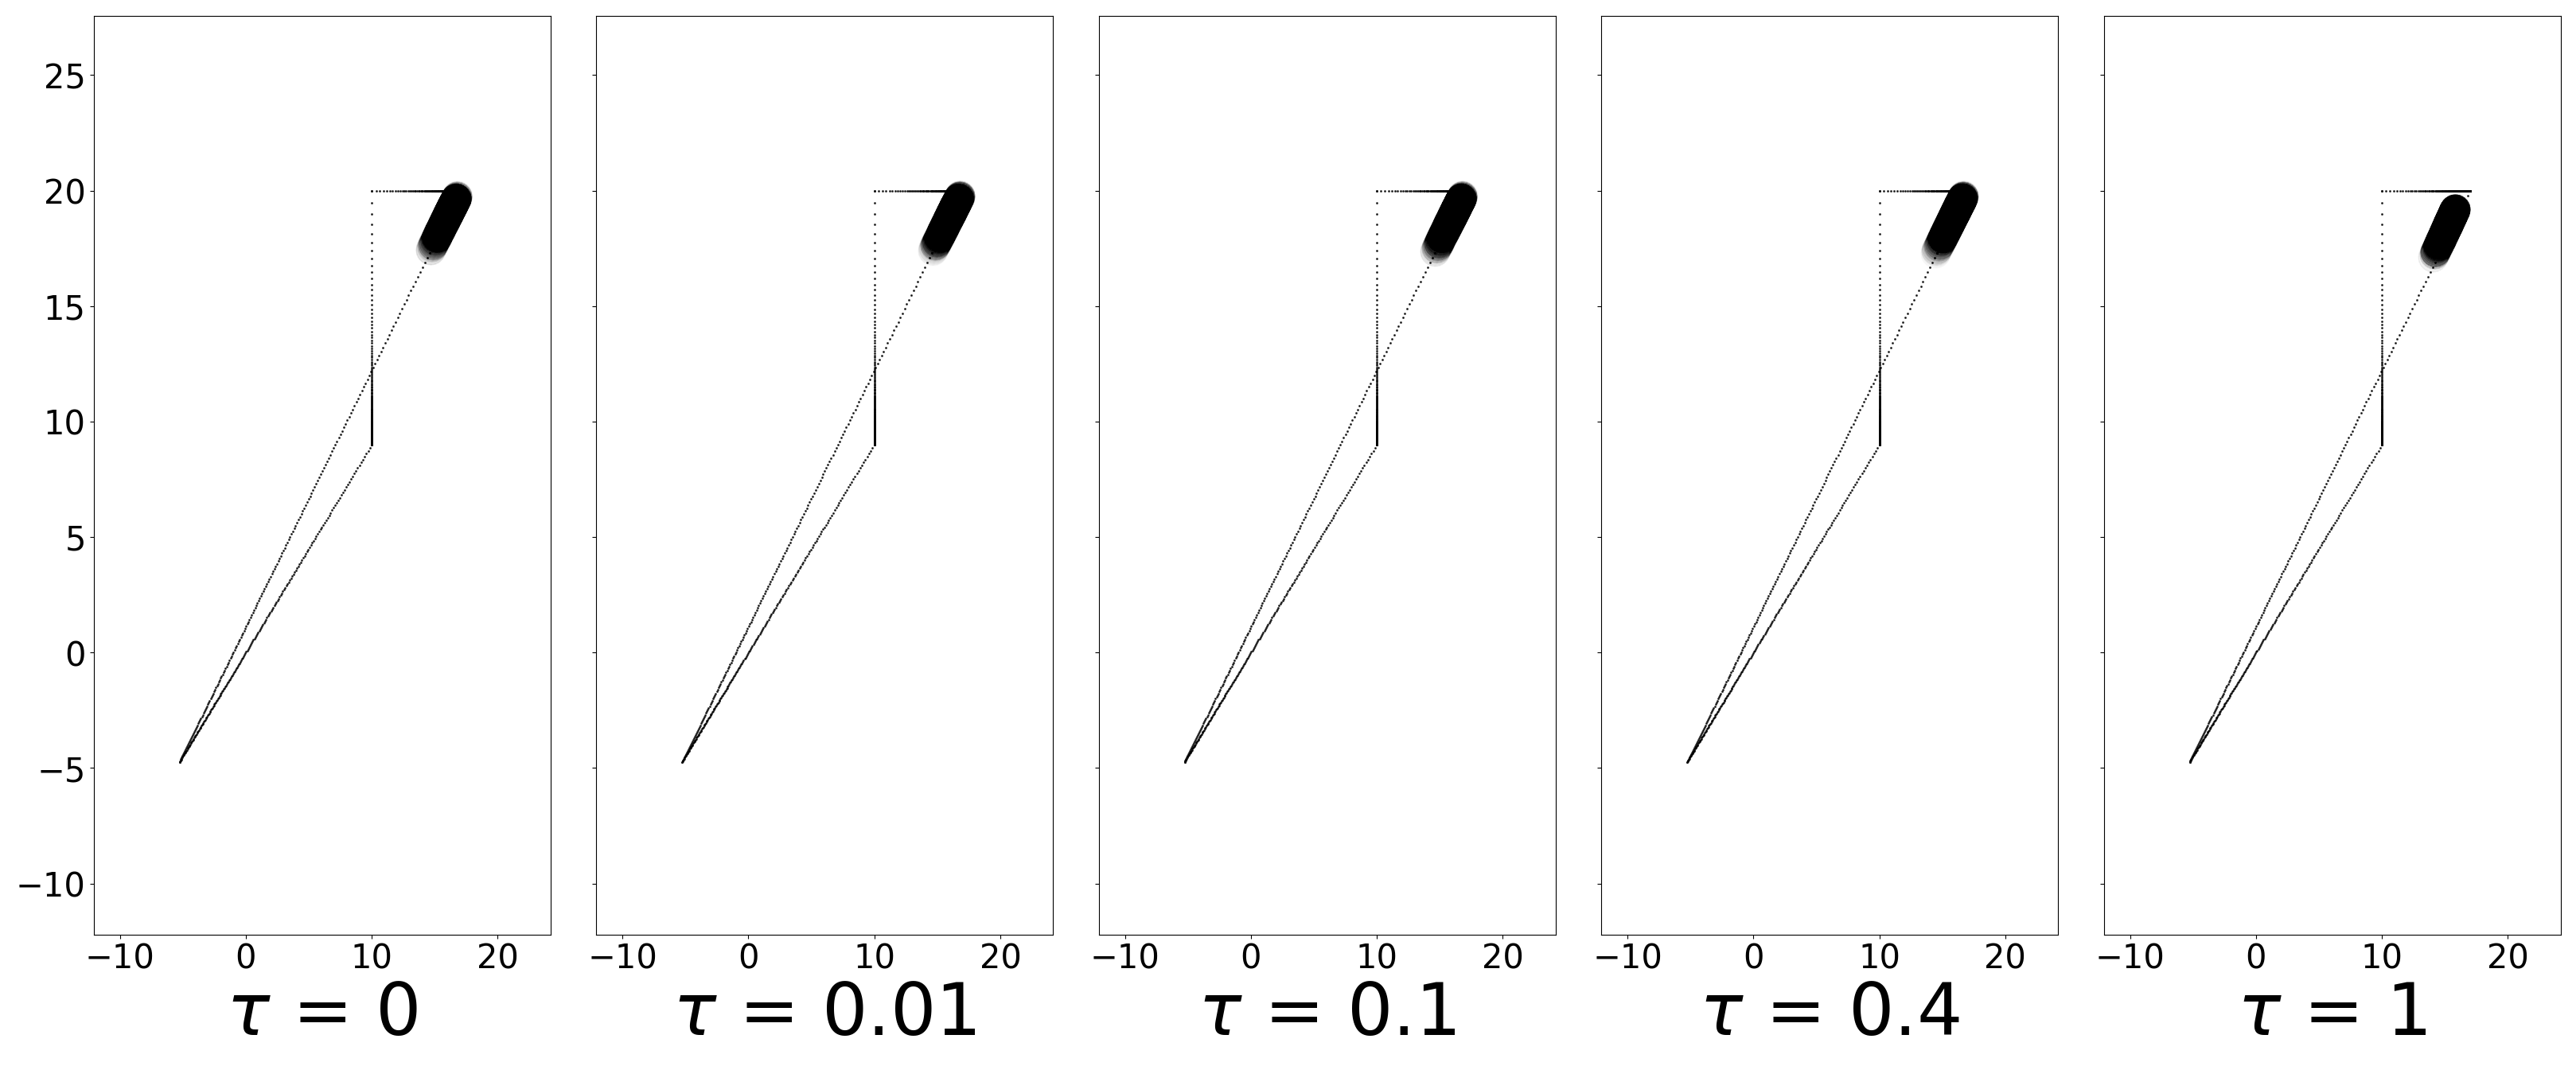
\includegraphics[width=0.8\columnwidth]{figs/switch-stay/notlearnQ/polytope_forward_optim=adam_lr=[0.01].png}
%     \caption{Forward KL, learning rate = 0.01.}
%     \label{fig:discrete-switch-stay-forward-adam0.01}
%   \end{subfigure}
  
%   \begin{subfigure}[b]{0.85\linewidth}
%         \centering
%         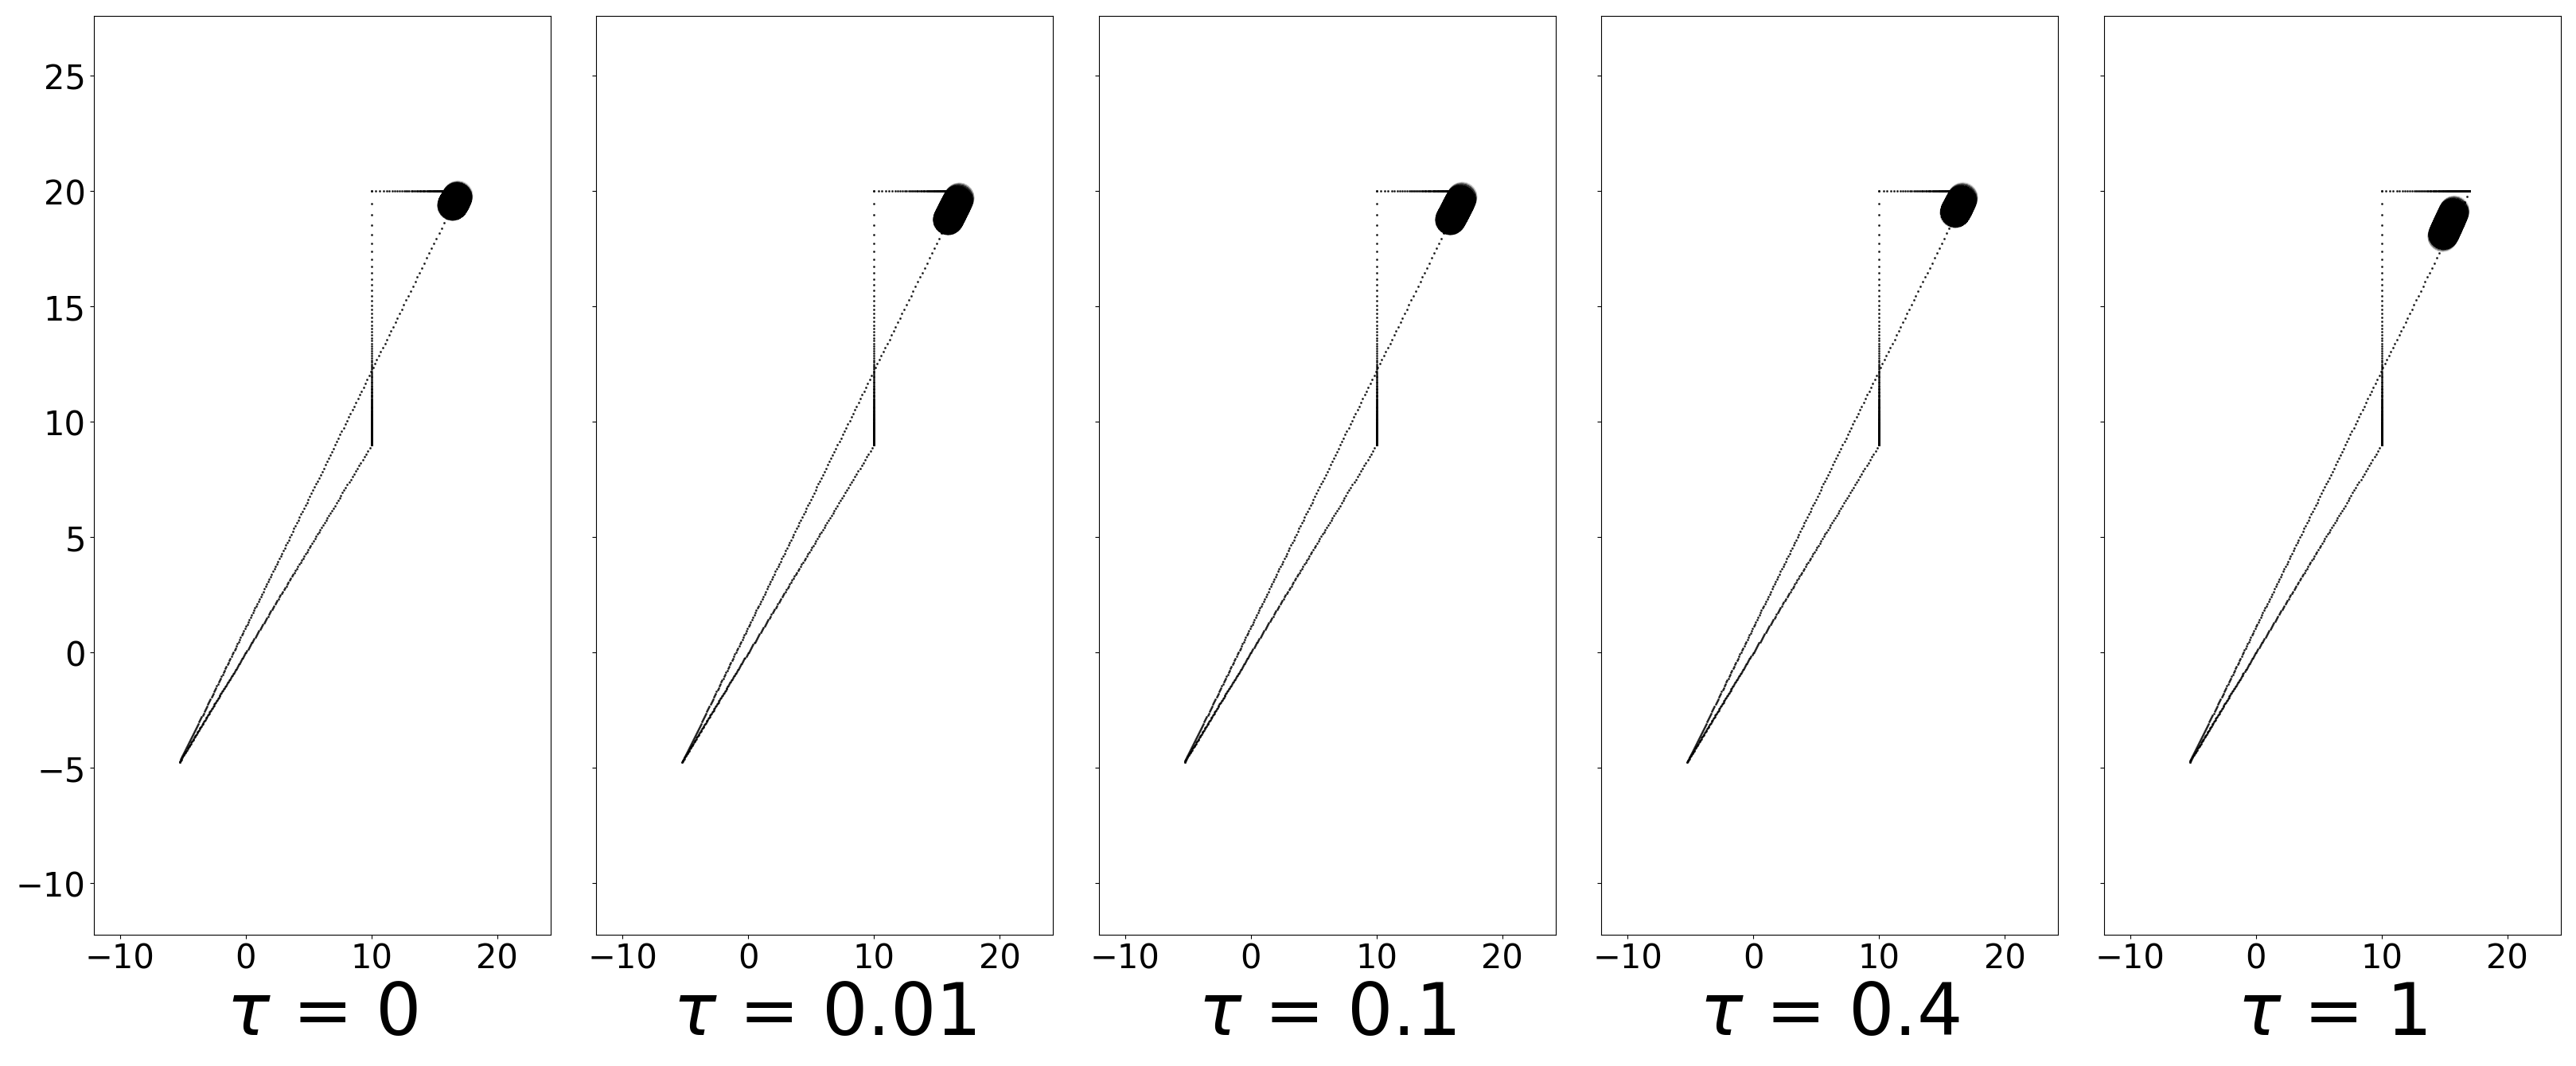
\includegraphics[width=0.8\columnwidth]{figs/switch-stay/notlearnQ/polytope_reverse_optim=adam_lr=[0.01].png}
%         \caption{Reverse KL, learning rate = 0.01.}
%         \label{fig:discrete-switch-stay-reverse-adam0.01}
%   \end{subfigure}
%   \caption{Final value functions on discrete version of switch-stay after 500 gradient steps, $\gamma = 0.9$. Using Adam for learning rates = $\{0.005, 0.01\}$.}
%   \label{fig:discrete-ss-all}
% \end{figure}


\begin{figure}[!htb]
  \centering
  \begin{subfigure}[b]{0.85\linewidth}
    \centering
    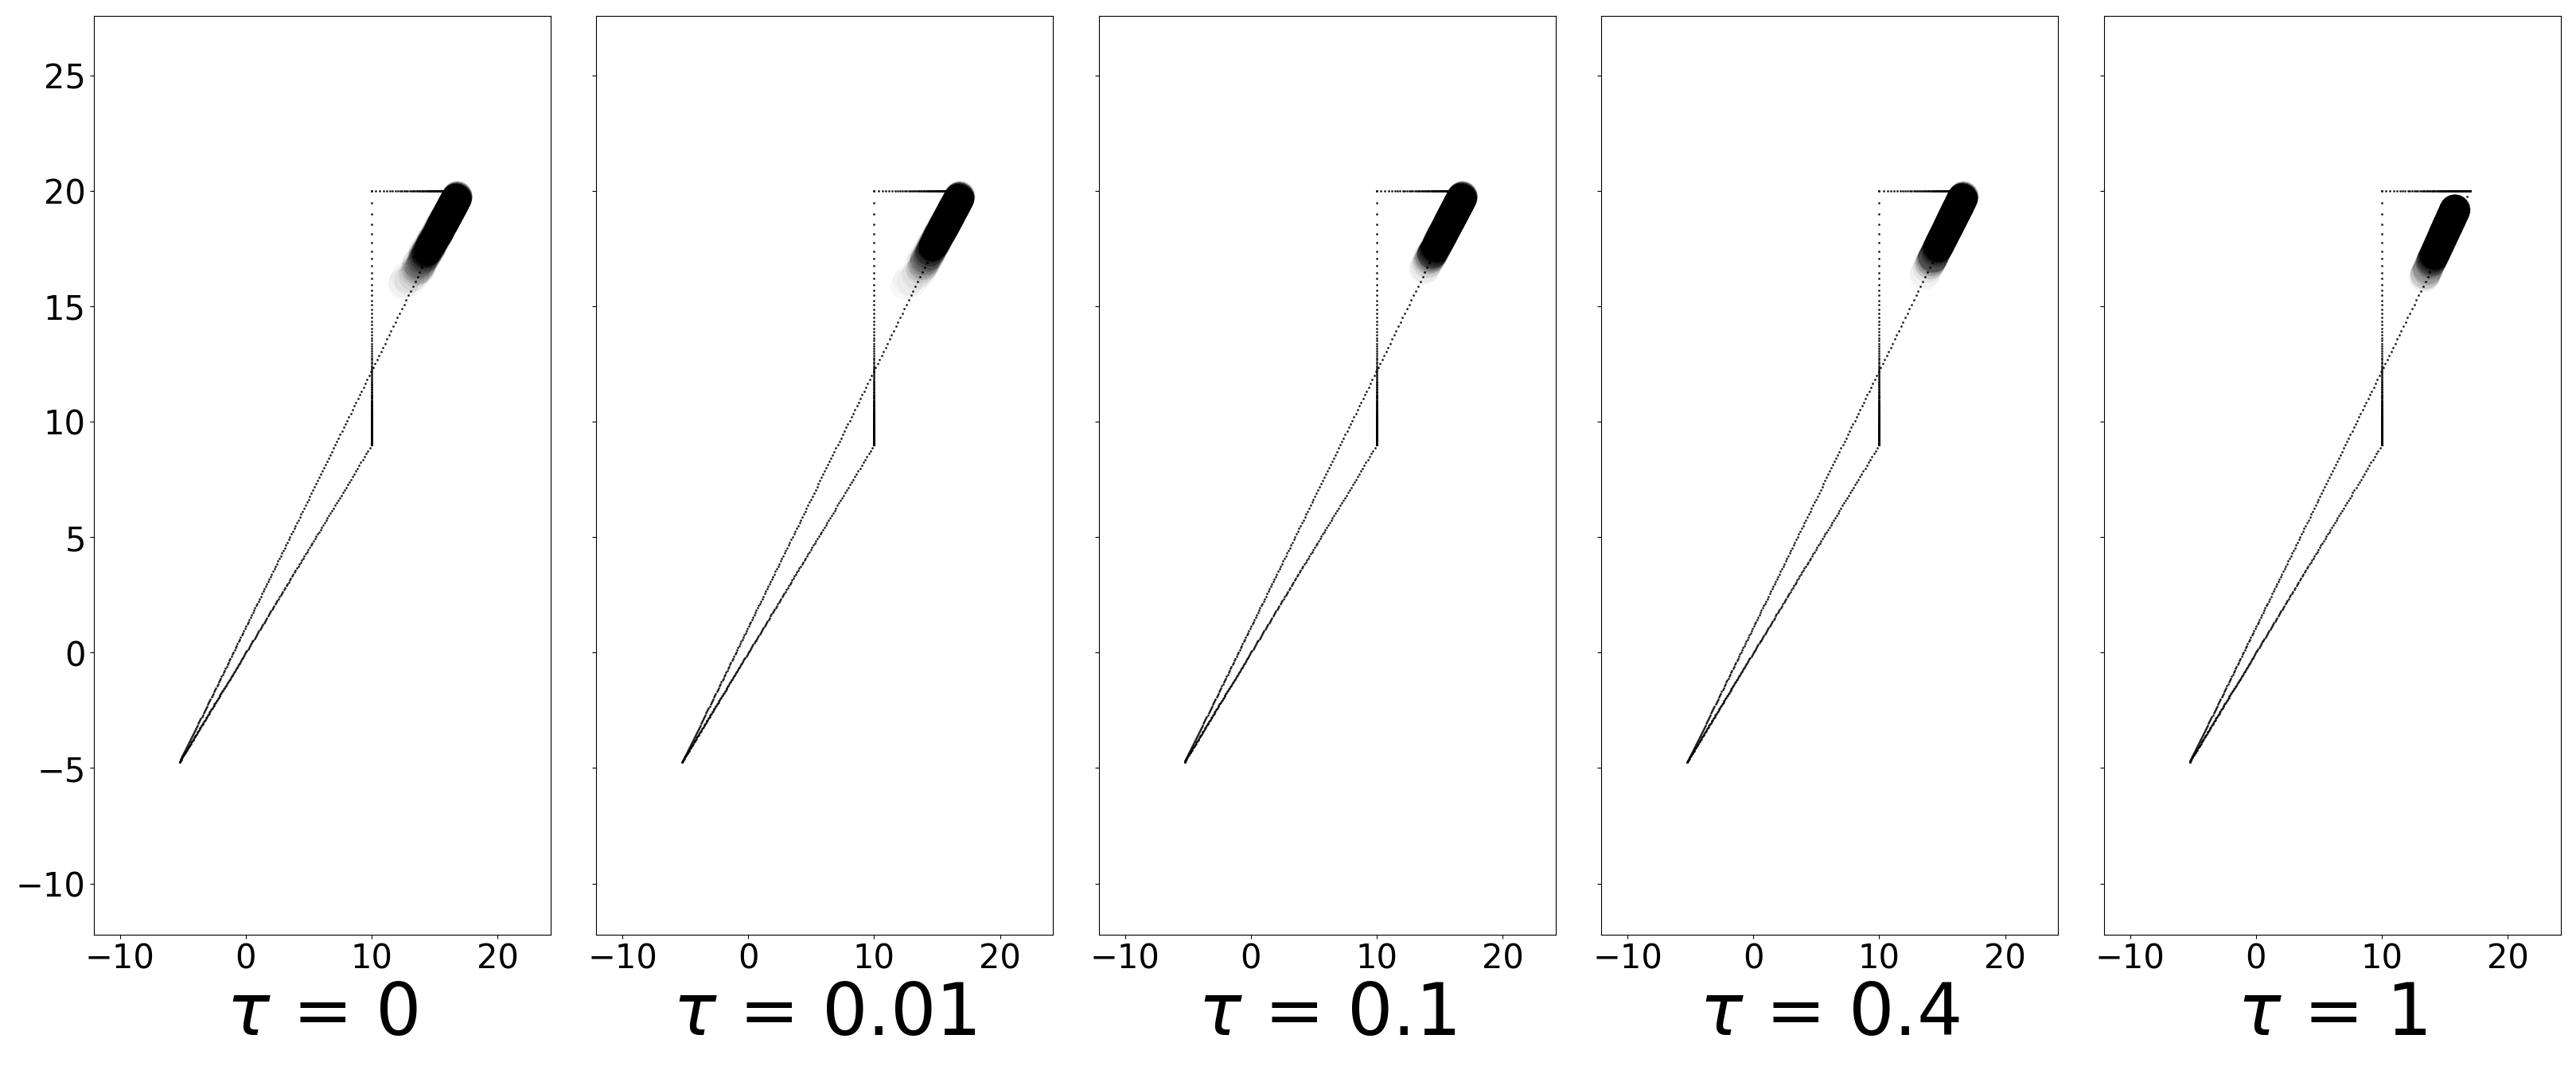
\includegraphics[width=0.8\columnwidth]{figs/switch-stay/notlearnQ/polytope_forward_optim=rmsprop_lr=[0.005].png}
    \caption{Forward KL, learning rate = 0.005.}
    \label{fig:discrete-switch-stay-forward-adam0.005}
  \end{subfigure}
  
  \begin{subfigure}[b]{0.85\linewidth}
        \centering
        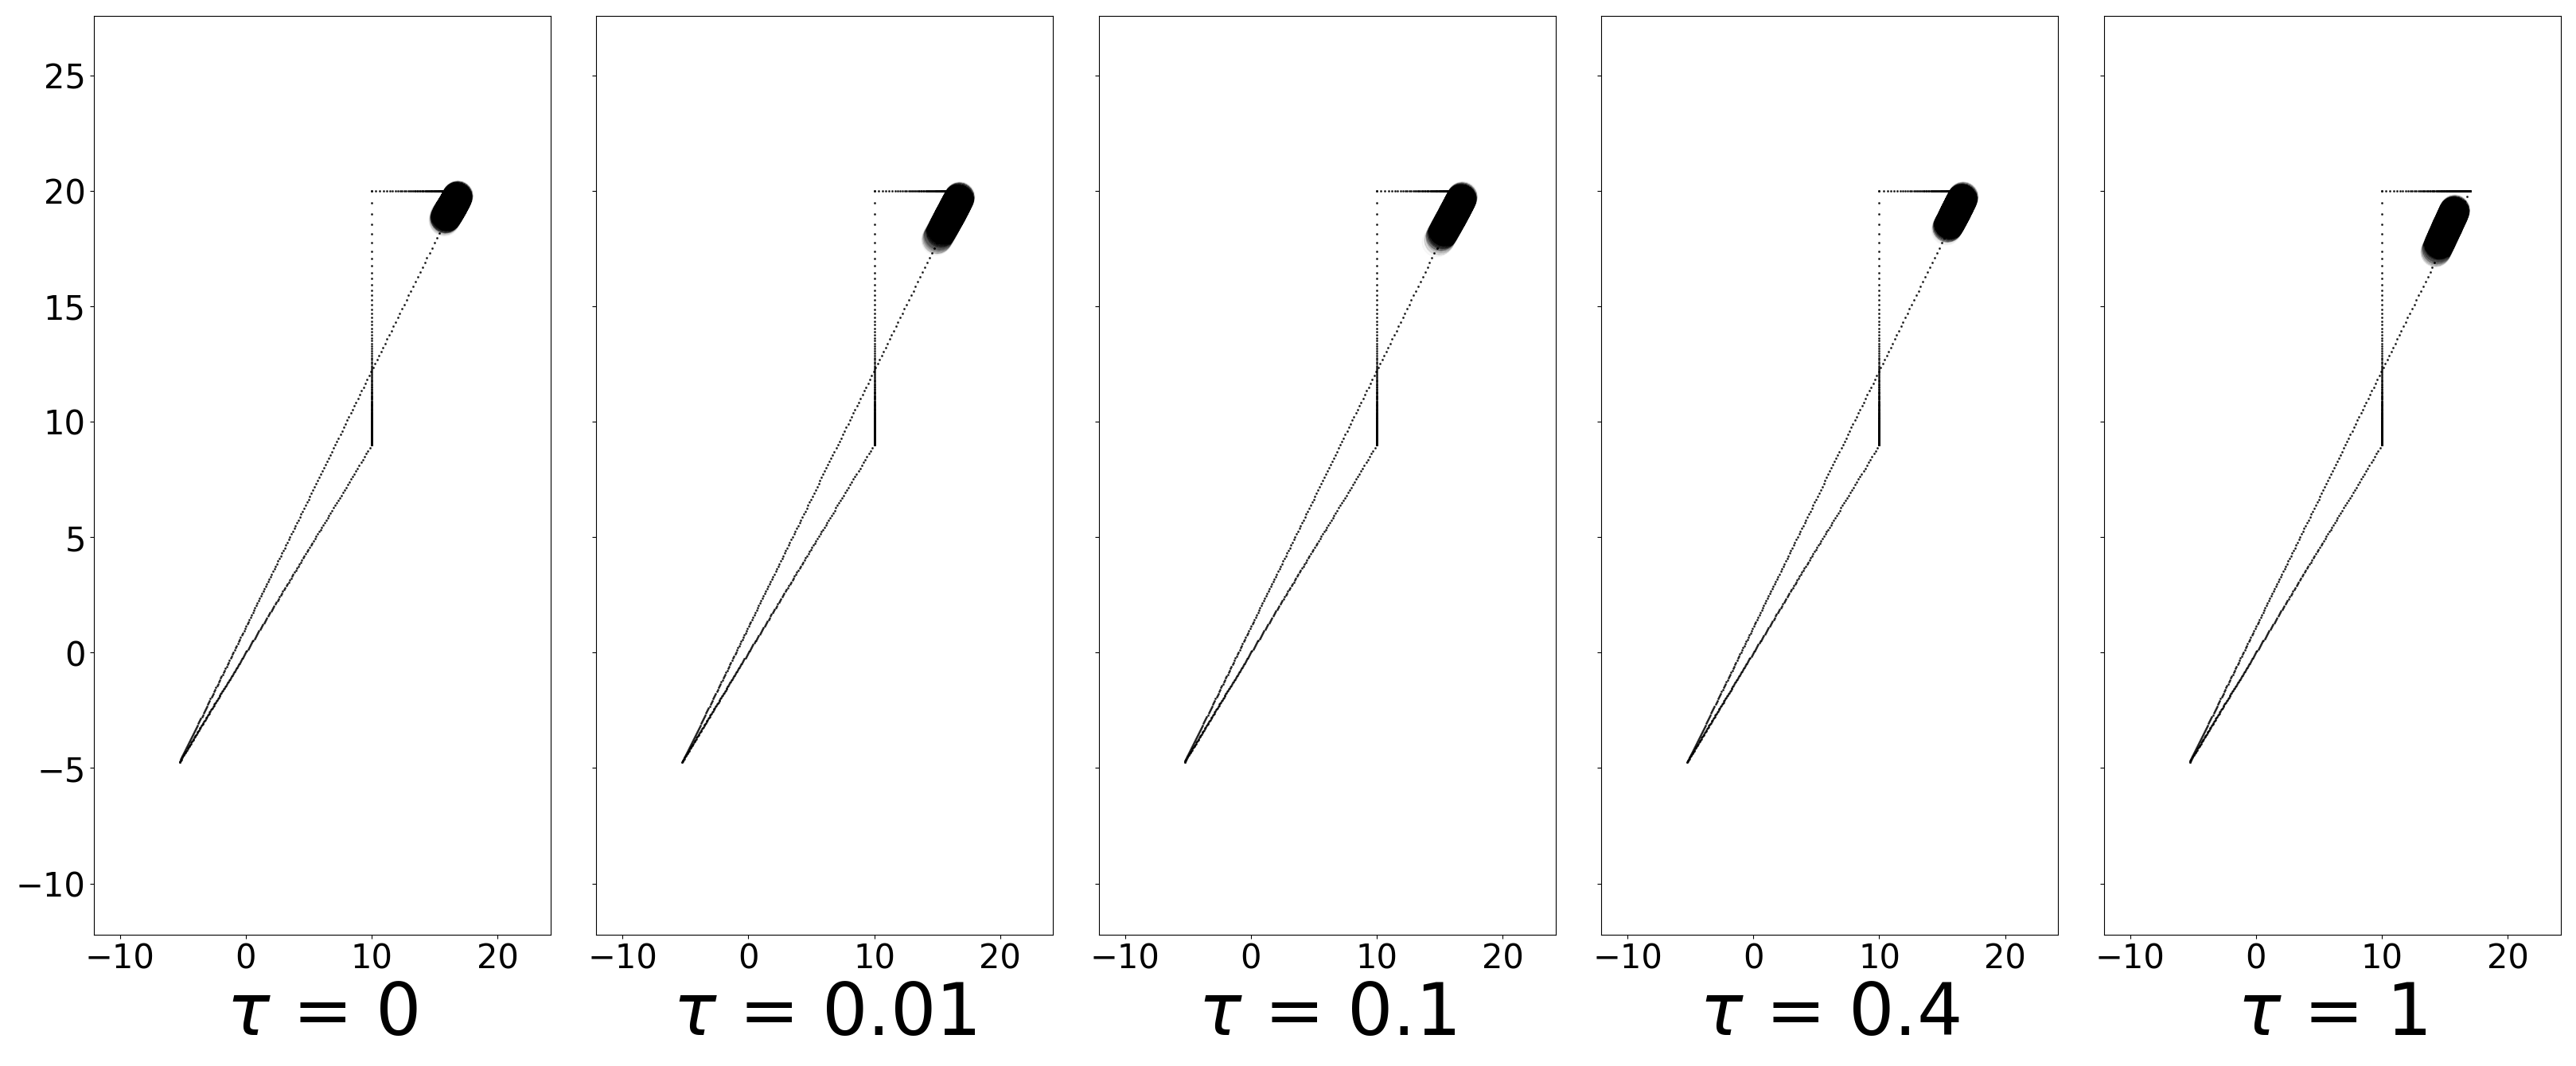
\includegraphics[width=0.8\columnwidth]{figs/switch-stay/notlearnQ/polytope_reverse_optim=rmsprop_lr=[0.005].png}
        \caption{Reverse KL, learning rate = 0.005.}
        \label{fig:discrete-switch-stay-reverse-adam0.005}
  \end{subfigure}
  
  \begin{subfigure}[b]{0.85\linewidth}
    \centering
    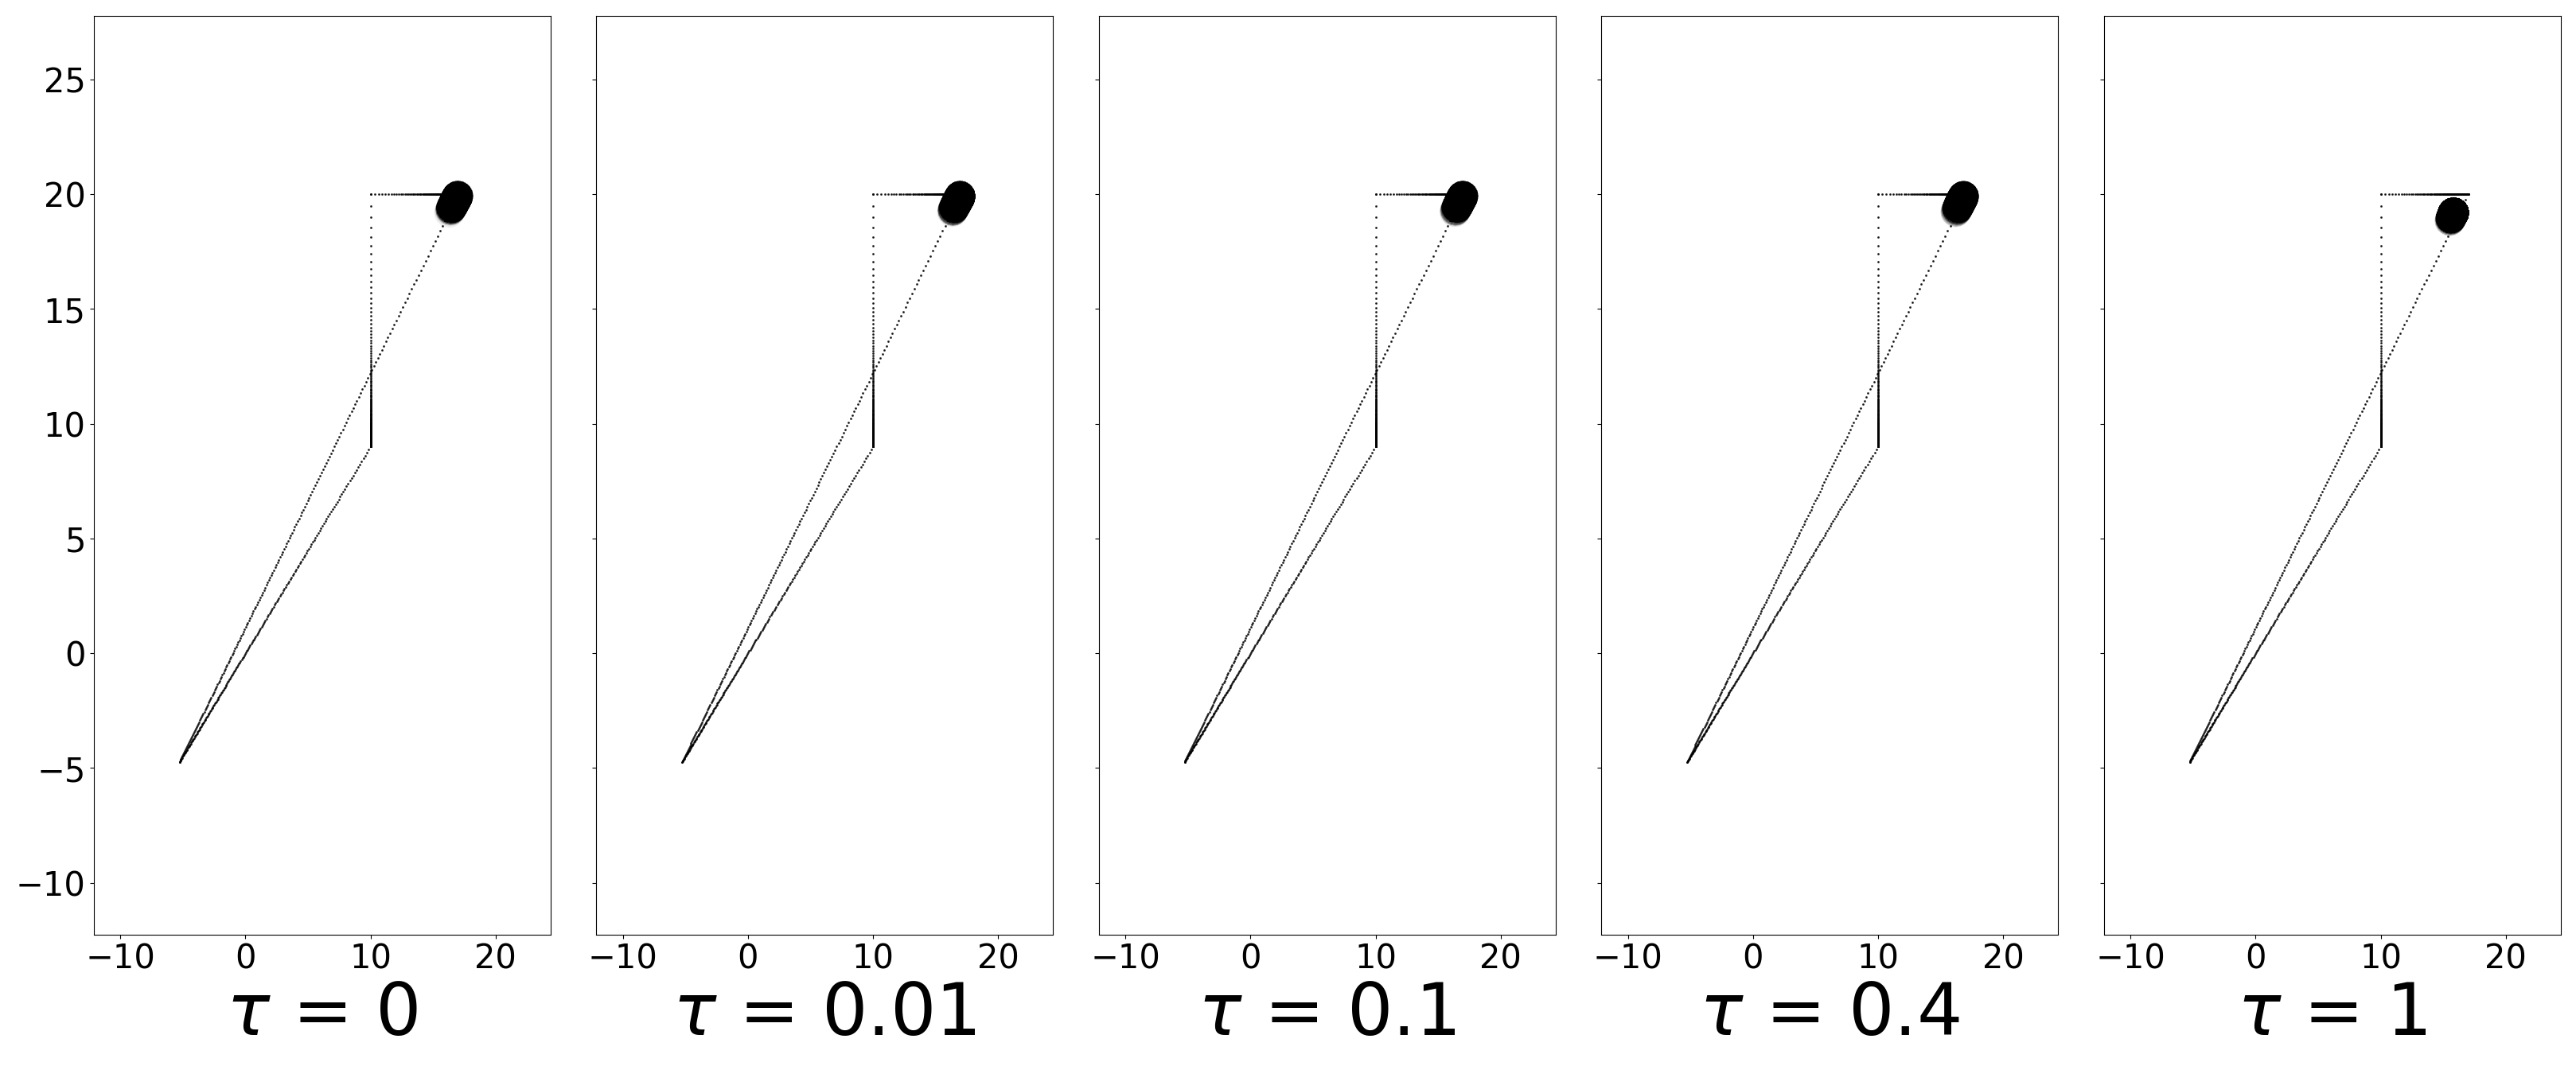
\includegraphics[width=0.8\columnwidth]{figs/switch-stay/notlearnQ/polytope_forward_optim=rmsprop_lr=[0.01].png}
    \caption{Forward KL, learning rate = 0.01.}
    \label{fig:discrete-switch-stay-forward-adam0.01}
  \end{subfigure}
  
  \begin{subfigure}[b]{0.85\linewidth}
        \centering
        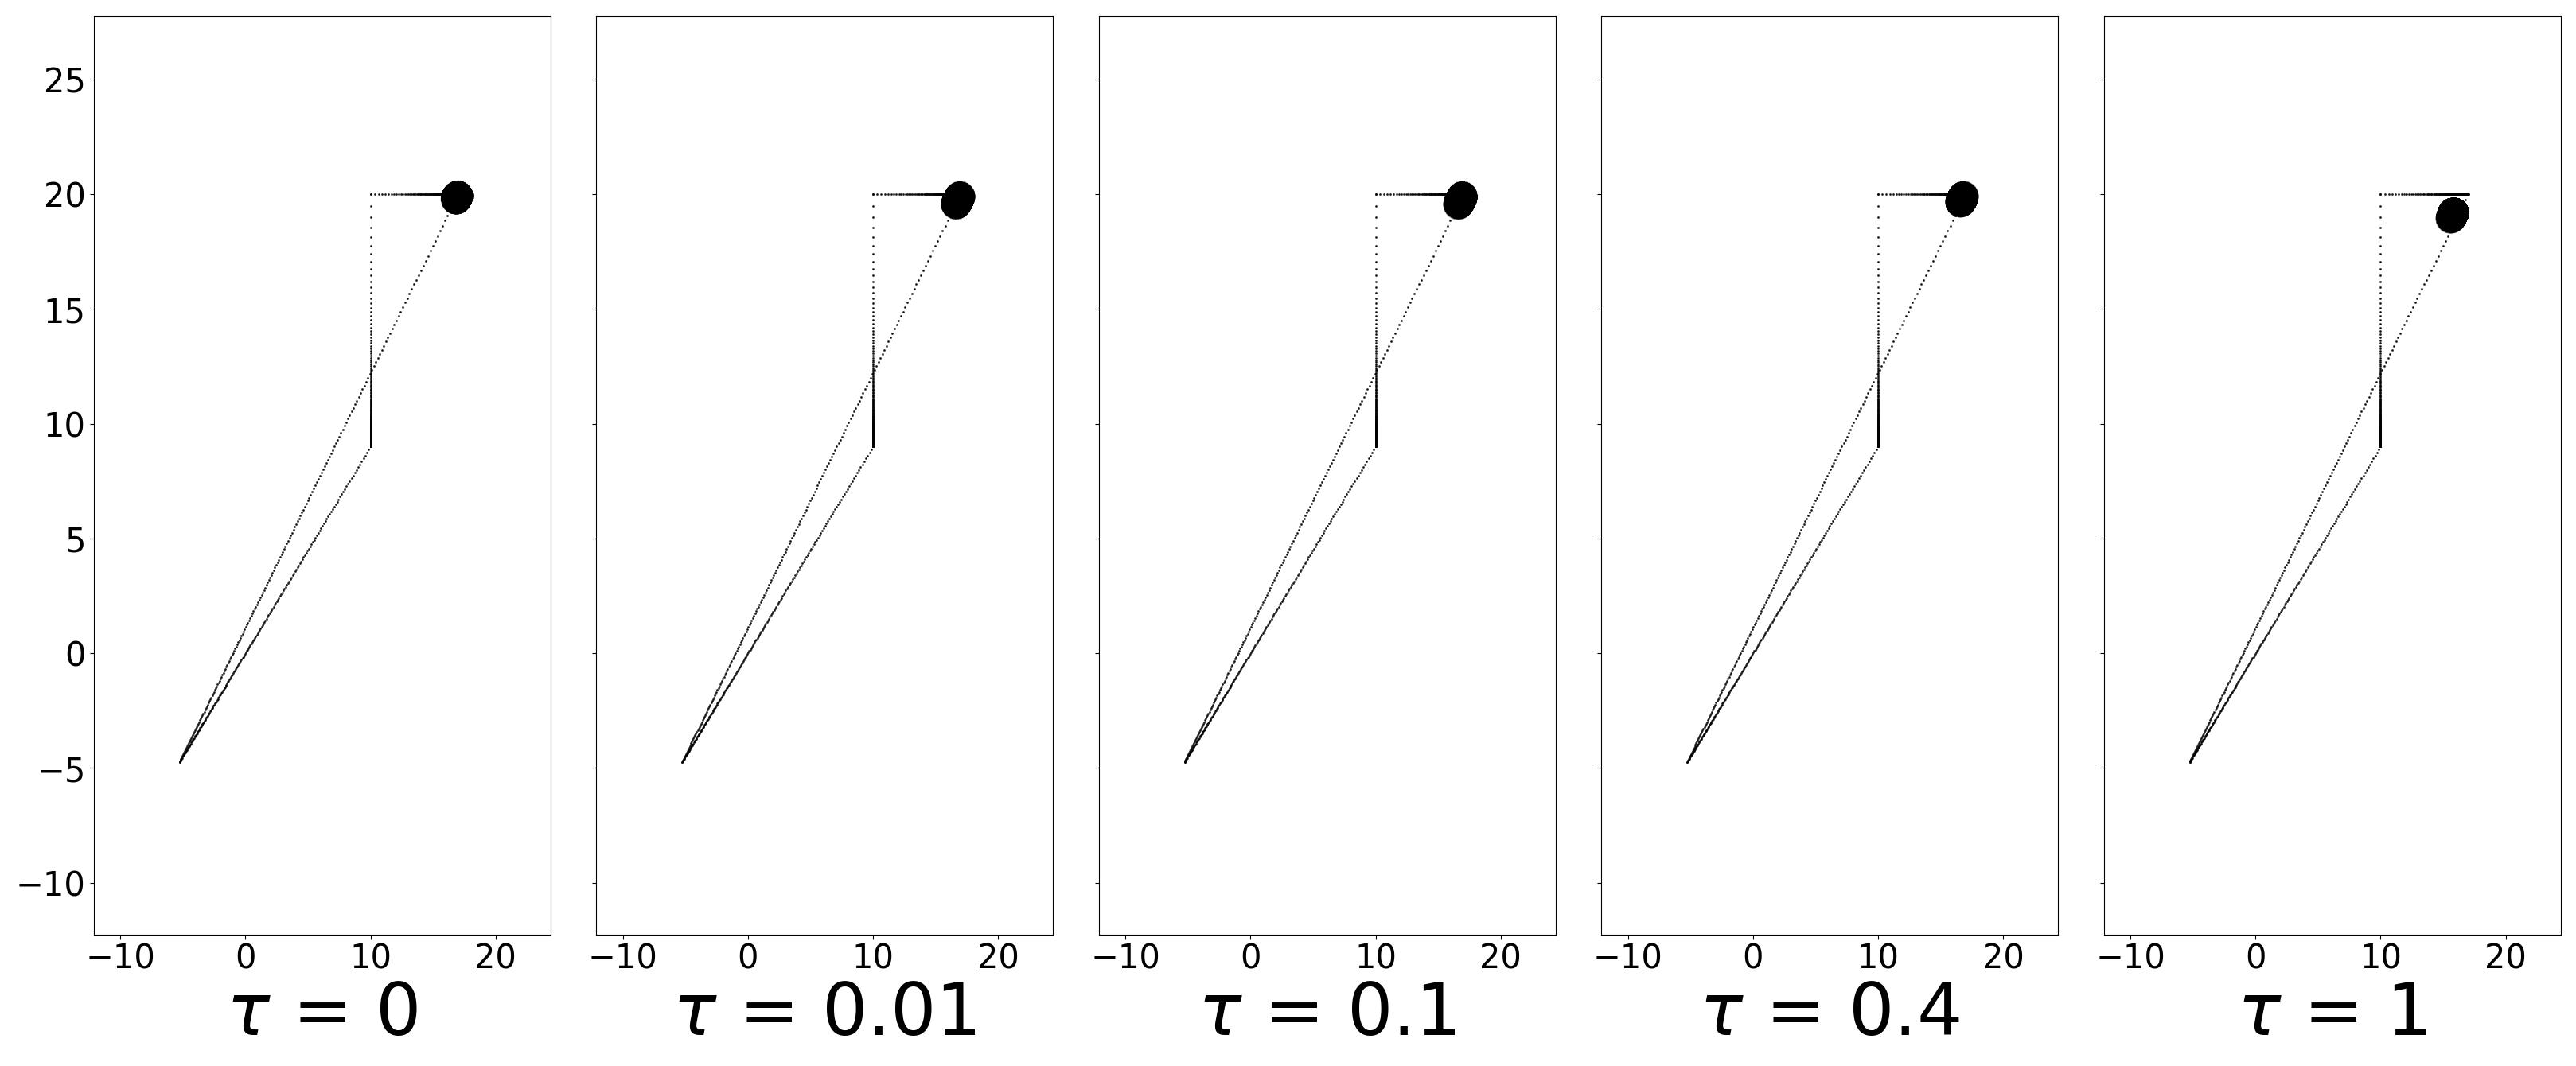
\includegraphics[width=0.8\columnwidth]{figs/switch-stay/notlearnQ/polytope_reverse_optim=rmsprop_lr=[0.01].png}
        \caption{Reverse KL, learning rate = 0.01.}
        \label{fig:discrete-switch-stay-reverse-adam0.01}
  \end{subfigure}
  \caption{Final value functions on discrete version of switch-stay after 500 gradient steps, $\gamma = 0.9$. Using RMSprop for learning rates $\in \{0.005, 0.01\}$.}
  \label{fig:discrete-ss-all}
\end{figure}


\section{The Impact of Stochasticity}\label{sec:stochastic-microworld}
Although with discrete actions it is practical to sum across all actions when calculating the KL losses, difficulty emerges with high-dimensional continuous action spaces. Quadrature methods scale exponentially with the dimension of the action-space, leaving methods like Clenshaw-Curtis impractical; Monte-Carlo integration seems the only feasible answer in this setting. 

We repeated the continuous-action microworld experiments to understand any differences induced by using Monte-Carlo integration (i.e., sampling actions from the current policy) instead of Clenshaw-Curtis quadrature to calculate the losses. 

Since Hard FKL only depends upon the maximum action, we do not modify the algorithm in this regime. Hard and soft RKL are modified to use sampled actions from the current policy $\pi$. To derive a sampling-based version of soft FKL, we use weighted importance sampling to approximate the integral $-\int_\actionspace \boltzmannQ(s, a) \log \pi(a \mid s)\, da$, noting that the omitted term $\entropy(\boltzmannQ(\cdot \mid s))$ does not depend on $\pi$. In particular, for samples $\{a_i\}_{i = 1}^n \sim \pi(\cdot \mid s)$ we estimate 
\begin{align*}
    -\int_\actionspace \boltzmannQ(s, a) \log \pi(a \mid s)\, da &\approx \sum_{i = 1}^n \rho_i \log \pi(a_i \mid s) ,\\
    \rho_i &:= \frac{\tilde{\rho}_i}{\sum_{j = 1}^n \tilde{\rho}_j}\\
    \tilde{\rho}_i &:= \frac{\exp(Q(s, a_i) \tau^{-1})}{\pi(a_i \mid s)}. 
\end{align*}
Note that we do not have to estimate $\entropy(\boltzmannQ(s, \cdot))$, the other term in the FKL, as it does not depend on $\pi$. Weighted importance sampling lets us avoid calculating the partition function in $\boltzmannQ$, and may be a fruitful avenue to explore in making FKL practical for high-dimensional action spaces. 

% \begin{figure}[!htb]
%   \centering
%   \begin{subfigure}[b]{0.85\linewidth}
%     \centering
%     \includegraphics[width=0.8\columnwidth]{figs/bandit/monte-carlo/10/mean_forward_optim=adam_modes=1_lr=0.005.png}
%     \caption{Forward KL.}
%     \label{fig:10-sample-cont-bandit-forward}
%   \end{subfigure}
  
%   \begin{subfigure}[b]{0.85\linewidth}
%         \centering
%         \includegraphics[width=0.8\columnwidth]{figs/bandit/monte-carlo/10/mean_reverse_optim=adam_modes=1_lr=0.005.png}
%         \caption{Reverse KL.}
%         \label{fig:10-sample-cont-bandit-reverse}
%   \end{subfigure}
%   \caption{Continuous bandit with 10 sample points, learning rate = 0.005, with Adam.}
% \end{figure}


\begin{figure}[!htb]
  \centering
  \begin{subfigure}[b]{0.85\linewidth}
    \centering
    \includegraphics[width=0.8\columnwidth]{figs/bandit/monte-carlo/10/mean_forward_optim=rmsprop_modes=1_lr=0.005.png}
    \caption{Forward KL.}
    \label{fig:10-sample-cont-bandit-forward}
  \end{subfigure}
  
  \begin{subfigure}[b]{0.85\linewidth}
        \centering
        \includegraphics[width=0.8\columnwidth]{figs/bandit/monte-carlo/10/mean_reverse_optim=rmsprop_modes=1_lr=0.005.png}
        \caption{Reverse KL.}
        \label{fig:10-sample-cont-bandit-reverse}
  \end{subfigure}
  \caption{Continuous bandit with 10 sample points, learning rate = 0.005, with RMSprop.}
\end{figure}


% \begin{figure}[!htb]
%   \centering
%   \begin{subfigure}[b]{0.85\linewidth}
%     \centering
%     \includegraphics[width=0.8\columnwidth]{figs/bandit/monte-carlo/100/mean_forward_optim=adam_modes=1_lr=0.005.png}
%     \caption{Forward KL.}
%     \label{fig:100-sample-cont-bandit-forward}
%   \end{subfigure}
  
%   \begin{subfigure}[b]{0.85\linewidth}
%         \centering
%         \includegraphics[width=0.8\columnwidth]{figs/bandit/monte-carlo/100/mean_reverse_optim=adam_modes=1_lr=0.005.png}
%         \caption{Reverse KL.}
%         \label{fig:100-sample-cont-bandit-reverse}
%   \end{subfigure}
%   \caption{Continuous bandit with 100 sample points, learning rate = 0.005, with Adam.}
% \end{figure}

% \begin{figure}[!htb]
%   \centering
%   \begin{subfigure}[b]{0.85\linewidth}
%     \centering
%     \includegraphics[width=0.8\columnwidth]{figs/bandit/monte-carlo/500/mean_forward_optim=adam_modes=1_lr=0.005.png}
%     \caption{Forward KL.}
%     \label{fig:500-sample-cont-bandit-forward}
%   \end{subfigure}
  
%   \begin{subfigure}[b]{0.85\linewidth}
%         \centering
%         \includegraphics[width=0.8\columnwidth]{figs/bandit/monte-carlo/500/mean_reverse_optim=adam_modes=1_lr=0.005.png}
%         \caption{Reverse KL.}
%         \label{fig:500-sample-cont-bandit-reverse}
%   \end{subfigure}
%   \caption{Continuous bandit with 500 sample points, learning rate = 0.005, with Adam.}
% \end{figure}


\begin{figure}[!htb]
  \centering
  \begin{subfigure}[b]{0.85\linewidth}
    \centering
    \includegraphics[width=0.8\columnwidth]{figs/bandit/monte-carlo/500/mean_forward_optim=rmsprop_modes=1_lr=0.005.png}
    \caption{Forward KL.}
    \label{fig:500-sample-cont-bandit-forward}
  \end{subfigure}
  
  \begin{subfigure}[b]{0.85\linewidth}
        \centering
        \includegraphics[width=0.8\columnwidth]{figs/bandit/monte-carlo/500/mean_reverse_optim=rmsprop_modes=1_lr=0.005.png}
        \caption{Reverse KL.}
        \label{fig:500-sample-cont-bandit-reverse}
  \end{subfigure}
  \caption{Continuous bandit with 500 sample points, learning rate = 0.005, with RMSprop.}
\end{figure}


While overall behaviour for the continuous bandit is consistent with the results using Clenshaw-Curtis quadrature, the iterates seem to cluster more slowly around their limit points, or not at all. 
% \textbf{Switch-Stay}

% \begin{figure}[!htb]
%   \centering
%   \begin{subfigure}[b]{0.85\linewidth}
%     \centering
%     \includegraphics[width=0.8\columnwidth]{figs/continuous-switch-stay/monte-carlo/10/polytope_forward_optim=adam_lr=0.01.png}
%     \caption{Forward KL.}
%     \label{fig:10-sample-switch-stay-forward}
%   \end{subfigure}
  
%   \begin{subfigure}[b]{0.85\linewidth}
%         \centering
%         \includegraphics[width=0.8\columnwidth]{figs/continuous-switch-stay/monte-carlo/10/polytope_reverse_optim=adam_lr=0.01.png}
%         \caption{Reverse KL.}
%         \label{fig:10-sample-switch-stay-reverse}
%   \end{subfigure}
%   \caption{Switch-stay with 10 sample points, learning rate = 0.01, with Adam.}
% \end{figure}

\begin{figure}[!htb]
  \centering
  \begin{subfigure}[b]{0.85\linewidth}
    \centering
    \includegraphics[width=0.8\columnwidth]{figs/continuous-switch-stay/monte-carlo/10/polytope_forward_optim=rmsprop_lr=0.01.png}
    \caption{Forward KL.}
    \label{fig:10-sample-switch-stay-forward}
  \end{subfigure}
  
  \begin{subfigure}[b]{0.85\linewidth}
        \centering
        \includegraphics[width=0.8\columnwidth]{figs/continuous-switch-stay/monte-carlo/10/polytope_reverse_optim=rmsprop_lr=0.01.png}
        \caption{Reverse KL.}
        \label{fig:10-sample-switch-stay-reverse}
  \end{subfigure}
  \caption{Switch-stay with 10 sample points, learning rate = 0.01, with RMSprop.}
\end{figure}

% \begin{figure}[!htb]
%   \centering
%   \begin{subfigure}[b]{0.85\linewidth}
%     \centering
%     \includegraphics[width=0.8\columnwidth]{figs/continuous-switch-stay/monte-carlo/100/polytope_forward_optim=adam_lr=0.01.png}
%     \caption{Forward KL.}
%     \label{fig:100-sample-switch-stay-forward}
%   \end{subfigure}
  
%   \begin{subfigure}[b]{0.85\linewidth}
%         \centering
%         \includegraphics[width=0.8\columnwidth]{figs/continuous-switch-stay/monte-carlo/100/polytope_reverse_optim=adam_lr=0.01.png}
%         \caption{Reverse KL.}
%         \label{fig:100-sample-switch-stay-reverse}
%   \end{subfigure}
%   \caption{Switch-stay with 100 sample points, learning rate = 0.01, with Adam.}
% \end{figure}

% \begin{figure}[!htb]
%   \centering
%   \begin{subfigure}[b]{0.85\linewidth}
%     \centering
%     \includegraphics[width=0.8\columnwidth]{figs/continuous-switch-stay/monte-carlo/500/polytope_forward_optim=adam_lr=0.01.png}
%     \caption{Forward KL.}
%     \label{fig:500-sample-switch-stay-forward}
%   \end{subfigure}
  
%   \begin{subfigure}[b]{0.85\linewidth}
%         \centering
%         \includegraphics[width=0.8\columnwidth]{figs/continuous-switch-stay/monte-carlo/500/polytope_reverse_optim=adam_lr=0.01.png}
%         \caption{Reverse KL.}
%         \label{fig:500-sample-switch-stay-reverse}
%   \end{subfigure}
%   \caption{Switch-stay with 500 sample points, learning rate = 0.01, with Adam.}
% \end{figure}


\begin{figure}[!htb]
  \centering
  \begin{subfigure}[b]{0.85\linewidth}
    \centering
    \includegraphics[width=0.8\columnwidth]{figs/continuous-switch-stay/monte-carlo/500/polytope_forward_optim=rmsprop_lr=0.01.png}
    \caption{Forward KL.}
    \label{fig:500-sample-switch-stay-forward}
  \end{subfigure}
  
  \begin{subfigure}[b]{0.85\linewidth}
        \centering
        \includegraphics[width=0.8\columnwidth]{figs/continuous-switch-stay/monte-carlo/500/polytope_reverse_optim=rmsprop_lr=0.01.png}
        \caption{Reverse KL.}
        \label{fig:500-sample-switch-stay-reverse}
  \end{subfigure}
  \caption{Switch-stay with 500 sample points, learning rate = 0.01, with RMSprop.}
\end{figure}


On Switch-Stay, more notable differences emerged. RKL iterates converged to minima to which they did not converge in the Clenshaw-Curtis regime, even for larger numbers of sample points. In \Cref{fig:500-sample-switch-stay-reverse}, there is an interesting trend across temperatures. Temperatures below $0.4$ induced many suboptima far from the optimal value function, while temperatures 0.4 and 1 seemed better at clustering RKL iterates near the optimal value function. On the other hand, FKL seemed relatively insensitive both to the temperature and the number of sample points. This relative insensitivity could be due to having a smoother loss landscape to begin with, which tends to direct iterates to a single global optimum. Nevertheless, that global optimum was often quite suboptimal with respect to the unregularized MDP, especially since many RKL iterates were much closer to the optimal policy of the unregularized MDP. 


\section{Summary}
Given the amount of data in this chapter, it is helpful to summarize our discussion thus far. 
\begin{enumerate}
    \item The relative difference between the KLs in continuous-action settings is larger than that in discrete-action settings. 
    \item On our bimodal bandit, the FKL was better at directing iterates to the global optimum, excepting some iterates that stayed near the suboptimal mode when the initial standard deviation was set sufficiently low. However, as the temperature increased, the global optimum of the FKL seemed to approach a suboptimal point with respect to the bandit reward function faster than the global optimum of the RKL did. 
    \item On the continuous version of Switch-Stay, the FKL iterates converged more slowly than the RKL iterates and to a policy that was less optimal, which seemed primarily due to a larger final standard deviation for the FKL iterates. The increased suboptimality of the FKL solution is consistent with our bandit results. 
    \item In the continuous-action setting, stochastic sampling of the loss function impacted RKL more than FKL. RKL tended to exhibit more spurious minima in this setting, even when increasing the number of sample points in the calculation of the loss. 
    \item In the discrete-action setting, little significant difference emerged between FKL and RKL. Both converged to nearly identical optima, although the convergence of iterates under FKL seemed slightly slower. 
\end{enumerate}

We suspect that the differences here are heavily due to the policy parameterization. One reason for the difference in the number of minima seems to be that a Gaussian policy is unimodal, whereas a softmax policy can represent multimodal distributions. As well, given that the behaviour in the bandit setting depended on the initial standard deviation, we hypothesize that the added complexity of learning the standard deviation contributes to the differences we observed between continuous and discrete actions. 


We also did not learn action-values in our experiments. Especially given the additional differences between the KLs that we observed with stochasticity, using learned action-values might drastically change our results. In this setting, the accuracy of the action-value estimate would depend on the actions taken by the agent, which in turn are affected by the process of policy optimization. For instance, if an agent tends to commit to an action at a given state and not try other actions, the resulting action-value estimate could be poor. In the literature in general, more investigation into the interplay of learning value functions and policy optimization is necessary. 

\end{document}